% !TEX encoding = UTF-8 Unicode
% !TEX TS-program = pdflatex
% !TEX root = arsclassica.tex
% !TEX spellcheck = it-IT

\documentclass[
              11pt,%                        % primary font size
              a4paper,%                     % A4
              %twoside,openright,%          % double sided
              oneside,openany,%             % only front
              titlepage,%                   % new page after the title
              %fleqn,%                      % position equations at a fixed indent from the left margin rather than centered in the text column (amsmath option)
              headinclude,,footinclude,%    % header at foot of the page
              BCOR5mm,%                     % 5 mm bookbinding
              numbers=noenddot,%            % no point after section number
              cleardoublepage=empty,%       % empty pages without header at foot of the page
              %tablecaptionabove,%          % captions above the tables
              %draft%                       % draft document
              ]{scrreprt}                   % KOMA class

\usepackage[T1]{fontenc}                    % font encoding: a complete LaTeX distribution is required

\usepackage{textcomp}                       % fix warning with missing font shapes

\usepackage{scrhack}                        % fix warnings when using KOMA with listings package

\usepackage{xspace}                         % to get the right spacing after macros

\usepackage[utf8]{inputenc}                 % input encoding: latin1 is also fine, it depends on the editor preferences

\usepackage[english,italian]{babel}         % add language if you need, e.g. [english, italian] so italian is the primary language

\usepackage[suftesi]{frontespizio}          % frontispiece
                                            % 1. compile arsclassica.tex
                                            % 2. compile arsclassica-frn.tex, generated by previous compilation
                                            % 3. compile arsclassica.tex again to include arsclassica-frn.pdf

\usepackage{indentfirst}                    % indent the first paragraph of each section

\usepackage{graphicx}                       % images

\usepackage{listings}                       % codes

\usepackage[font=small]{quoting}            % text citations

\usepackage{amsmath,amssymb,amsthm,amsfonts}% math

\usepackage[italian]{varioref}              % completed references

\usepackage{mparhack,fixltx2e,relsize}      % typographical niceties

\usepackage[printonlyused,
            smaller,
            withpage]{acronym}              % acronyms

\usepackage{tabularx}                       % tabelle di larghezza prefissata

\usepackage[babel,
            italian=guillemets]{csquotes}   % automates some stylistic choices language-dependent: using \mkbibquote command you will get caporali quotes (i.e. « »)

\usepackage[style=philosophy-modern,
            hyperref,backref,natbib,
            backend=biber]{biblatex}        % bibliography:
                                            % philosophy-modern for author-year citation style
                                            % add square option after backref option to get square brackets
                                            % numeric-comp for numeric citation style

\bibliography{bibliography}                 % bibliography database

\usepackage{subfig}                         % subfigures, subtables

\usepackage{lipsum}                         % placeholding text

\usepackage{kbordermatrix}

\usepackage{rotating}

\usepackage{float}

\usepackage[export]{adjustbox}

\usepackage{eurosym}

\usepackage{mathrsfs}

% ********************************************************************
% Available options for classicthesis.sty:
% drafting
% parts nochapters linedheaders
% eulerchapternumbers beramono eulermath pdfspacing minionprospacing
% tocaligned dottedtoc manychapters
% listings floatperchapter subfig
% ********************************************************************
\usepackage[eulerchapternumbers,%           % chapter numbers font: Euler
            subfig,%                        % because subfig packages has been loaded
            %minionpro,%                    %
            beramono,%                      % fixed-width font: Bera Mono
            eulermath,%                     % math font: AMS Euler
            pdfspacing,%                    % better line filling
            listings,%                      % listings
            %parts,%                        % document divided into parts, not chapters
            dottedtoc,%                     % align TOC page numbers to right
            floatperchapter                 % float objects numbered by chapter
            ]{classicthesis}                % classicthesis style


\usepackage{arsclassica}                    % improve classicthesis

\usepackage{etoolbox}

\usepackage[noabbrev,italian]{cleveref}

\usepackage{chngcntr}

\usepackage{imakeidx}                       % analitycal index

\usepackage{multicol}

\usepackage{siunitx}                        % units

\usepackage{keyval,xparse}

\usepackage{xstring}

\usepackage{bookmark}

%******************************************************************
% Settings
%******************************************************************
% !TEX encoding = UTF-8 Unicode
% !TEX TS-program = pdflatex
% !TEX root = arsclassica.tex
% !TEX spellcheck = it-IT

%*********************************************************************************
% Comandi personali
%*********************************************************************************
\newcommand{\myname}{Leonardo Di Donato}
\newcommand{\myid}{744739}
\newcommand{\mytitle}{Continuos Time Bayesian Network Classifiers}
\newcommand{\mysplittedtitle}{Continuos Time \\ Bayesian Network Classifiers}
\newcommand{\mysubtitle}{}
\newcommand{\mydegree}{Tesi di Laurea Magistrale}
\newcommand{\mycourse}{Informatica}
\newcommand{\myuni}{Milano-Bicocca}
\newcommand{\myfaculty}{Scienze Matematiche, Fisiche e Naturali}
\newcommand{\mydepartment}{Dipartimento di Informatica, Sistemistica e Comunicazione}
\newcommand{\myprof}{Prof.~Fabio Stella}
\newcommand{\mycorrelator}{Dott.~Daniele Codecasa}
\newcommand{\mylocation}{Milano}
\newcommand{\mytime}{settembre 2013}
\newcommand{\myaa}{2012-2013}
\newcommand{\mysubject}{Continuos time Bayesian Network Classifiers}
\newcommand{\mykeywords}{Learning, Inference, Classification, Structural Learning, Continuos time Bayesian Network, CTBN, Continuos time Bayesian Newtork Classifier, CTBNC, Classifiers, Bayesian Classifiers, Machine Learning}
\newcommand{\mail}[1]{\href{mailto:#1}{\texttt{#1}}}

% !TEX encoding = UTF-8 Unicode
% !TEX TS-program = pdflatex
% !TEX root = arsclassica.tex
% !TEX spellcheck = it-IT

%*********************************************************************************
% Preamble
%*********************************************************************************

\sisetup{output-decimal-marker={,}}

%*********************************************************************************
% TOC settings
%*********************************************************************************
% \setcounter{secnumdepth}{5}
% \setcounter{tocdepth}{5}

%*********************************************************************************
% Chapters style
%*********************************************************************************
% Chapter number style: decomment if you want it with the same corpus font
% \renewcommand{\chapterNumber}{%
% \fontsize{70}{70}\usefont{\encodingdefault}{\sfdefault}{b}{n}%
% }%

% Workaround: multi-line titles
\renewcommand\formatchapter[1]{%
\begin{minipage}[b]{0.15\linewidth}
\chapterNumber
\end{minipage}%
\begin{minipage}[b]{0.70\linewidth}%length of the second row
\raggedright\spacedallcaps{#1}
\end{minipage}
}

%*********************************************************************************
% Impostazioni di amsmath, amssymb, amsthm
%*********************************************************************************

\DeclareMathAlphabet{\mathscrbf}{OMS}{mdugm}{b}{n}
\newcommand{\myinitial}{\mathscrbf{L}}

% Force the equation numbers to be always the same size
\makeatletter
\renewcommand{\maketag@@@}[1]{\hbox{\m@th\normalsize\normalfont#1}}%
\makeatother

% operators
\DeclareMathOperator*{\argmax}{arg\,max}
\DeclareMathOperator*{\argmin}{arg\,min}

% comandi per gli insiemi numerici (serve il pacchetto amssymb)
\newcommand{\numberset}{\mathbb}
\newcommand{\N}{\numberset{N}}
\newcommand{\R}{\numberset{R}}

% comandi per gli insiemi
\newcommand{\set}[1]{\mathbf{#1}}
\newcommand{\setel}[1]{\mathnormal{#1}}  % o \mathrm o \mathit

% comandi per i vettori
\newcommand{\vect}[1]{\set{#1}}
\newcommand{\vectel}[1]{\mathrm{#1}}

% comandi per i simboli matematici che denotano schemi, categorie, concetti
\newcommand{\conceptsym}[1]{\mathcal{#1}} % or use pazocal % try it

% un ambiente per i sistemi
\newenvironment{sistema}%
  {\left\lbrace\begin{array}{@{}l@{}}}%
  {\end{array}\right.}

% comandi per le lettere greche
% ...

% reference for equation terms. e.g., \tag*{\myterm{termA}}
\newcounter{term}
\renewcommand*{\theterm}{(\emph{\alph{term}})}
\AtBeginDocument{%
  \let\mylabel\label
}
\newcommand{\myterm}[1]{%
  \begingroup % keep the effects of \refstepcounter local
    \refstepcounter{term}%
    \mylabel{#1}%
    \text{\theterm}%
  \endgroup
}

%*********************************************************************************
% Nuovi ambienti: definizioni, teoremi etc. etc.
%*********************************************************************************
% definizioni (serve il pacchetto amsthm)
\newtheoremstyle{classicdef}% Nome
{12pt}% Spazio che precede l�enunciato
{12pt}% Spazio che segue l�enunciato
{}% Stile del font dell�enunciato
{}% Rientro (se vuoto, non c�� rientro,
% \parindent = rientro dei capoversi)
{\scshape}% Stile del font dell�intestazione
{:}% Punteggiatura che segue l�intestazione
{.5em}% Spazio che segue l�intestazione:
% " " = normale spazio inter-parola;
% \newline = a capo
{}% Specifica l�intestazione dell�enunciato
% (normalmente viene lasciata vuota)

\theoremstyle{definition}
\newtheorem{definizione}{Definizione}[chapter]
% \newtheorem{osservazione}[definizione]{Osservazione}
% \newtheorem{definizione}{Definizione}[section]
\newtheorem{osservazione}{Osservazione}[definizione]

% esempi
\theoremstyle{definition}
\newtheorem{esempio}{Esempio}[definizione]

% note about definitions
\theoremstyle{remark}
\newtheorem{notabene}{Nota}[definizione]

% note of section
\theoremstyle{remark}
\newtheorem{nota}{Nota}[section]

\theoremstyle{remark}
\newtheorem{notas}{Nota}[subsection]

% teoremi (serve il pacchetto amsthm)
\newtheoremstyle{classicthm}% Nome
{12pt}% Spazio che precede l�enunciato
{12pt}% Spazio che segue l�enunciato
{\itshape}% Stile del font dell�enunciato
{}% Rientro (se vuoto, non c�� rientro,
% \parindent = rientro dei capoversi)
{\scshape}% Stile del font dell�intestazione
{:}% Punteggiatura che segue l�intestazione
{.5em}% Spazio che segue l�intestazione:
% " " = normale spazio inter-parola;
% \newline = a capo
{}% Specifica l�intestazione dell�enunciato
% (normalmente viene lasciata vuota)

\theoremstyle{plain}
\newtheorem{teorema}{Teorema}[chapter]
\newtheorem*{teorema*}{Teorema}
\newtheorem{cor}[teorema]{Corollario}
\newtheorem{lem}[teorema]{Lemma}
\newtheorem{prop}[teorema]{Proposizione}
\newtheorem{oss}[teorema]{Osservazione}

% leggi (serve il pacchetto amsthm)
\newtheorem{legge}{Legge}
\newtheorem{decreto}[legge]{Decreto}

%*********************************************************************************
% Impostazioni di acronym
%*********************************************************************************
\newcommand{\acroname}{Acronimi}
% \renewcommand*{\acsfont}[1]{\textssc{#1}}                 % for MinionPro
\renewcommand*{\acsfont}[1]{\textsmaller{#1}}               % customize font for long version acronyms [works only if footnote not activate]
\renewcommand*{\acffont}[1]{#1}                             % idem, but for short version of acronyms
\renewcommand{\bflabel}[1]{{#1}\hfill}                      % fix the list of acronyms
\makeatletter                                               % macro that tweeks acronym package to render lowercase or not
\newif\if@in@acrolist
\AtBeginEnvironment{acronym}{\@in@acrolisttrue}
\newrobustcmd{\ul}[2]{\if@in@acrolist#1\else#2\fi}          % \ul{C}{c}iao defines an uppercase and lowercase variant of the same acronym
\newcommand{\ACF}[1]{{\@in@acrolisttrue\acf{#1}}}           % \ACF{<acronym>} force the defined capitalized variants of acronym letters/words
\newcommand{\ACL}[1]{{\@in@acrolisttrue\acl{#1}}}           % \ACL{<acronym}
\makeatother

%*********************************************************************************
% Impostazioni di biblatex
%*********************************************************************************
\defbibheading{bibliography}{%
\cleardoublepage
\manualmark
\phantomsection
\addcontentsline{toc}{chapter}{\tocEntry{\bibname}}
\chapter*{\bibname\markboth{\spacedlowsmallcaps{\bibname}}
{\spacedlowsmallcaps{\bibname}}}}

%*********************************************************************************
% Impostazioni di listings
%*********************************************************************************

% extract text between square brackets
\DeclareRobustCommand{\getsquarebrackscontent}[1]{%
  \StrBetween[1,1]{#1}{[}{]}%
}
\DeclareRobustCommand{\getshort}[1]{%
  \sbox0{\getsquarebrackscontent{#1}}%
  \ifdim\wd0=0pt
    {#1}% if #1 is empty
  \else
    {\getsquarebrackscontent{#1}}% if #1 is not empty
  \fi
}

% Input source code
\makeatletter
\newcommand{\sourcecodename}{Sorgente}
\let\oldaddcontentsline\addcontentsline
\newcommand{\listofsourcecodename}{Elenco dei sorgenti}%
\lst@UserCommand\listofsourcecode{\bgroup
  \let\contentsname\listofsourcecodename
  \let\lst@temp\@starttoc \def\@starttoc##1{\lst@temp{los}}
  \newlength{\sourcecodelabelwidth}
  \settowidth{\sourcecodelabelwidth}{\sourcecodename~999}
  \addtolength{\sourcecodelabelwidth}{1.8em}
  \def\l@lstlisting##1##2{\@dottedtocline{1}{0em}{\sourcecodelabelwidth}{##1}{##2}}
  \def\numberline##1{\hb@xt@\@tempdima{\sourcecodename{} ##1\hfil}}
  \tableofcontents \egroup}%
\newcommand{\inputsourcecode}[2][]{{%
  \renewcommand{\lstlistingname}{\sourcecodename}%
  \renewcommand{\addcontentsline}[3]{\oldaddcontentsline{los}{##2}{##3}}%
  \lstinputlisting[#1]{#2}%
}}
\makeatother

%\newcommand{\sourcecodename}{Sorgente}
%\newcommand{\listofsourcecodename}{Elenco dei sorgenti}
%\newlistof[chapter]{sourcecode}{los}{\listofsourcecodename}%
%\renewcommand{\cftsourcecodefont}{\normalfont}%
%\renewcommand{\cftsourcecodepresnum}{\lstlistingname~}%
%\renewcommand{\cftsourcecodepagefont}{\normalfont}%
%\renewcommand{\cftsourcecodepresnum}{\sourcecodename~}%
%\cftsetindents{sourcecode}{0em}{\figurelabelwidth}%
%\makeatletter
%  \let\oldaddcontentsline\addcontentsline
%  \newcommand{\inputsourcecode}[2][]{%
%    \refstepcounter{sourcecode}
%    \renewcommand{\lstlistingname}{\sourcecodename}%
%    \def\numberline##1{\hb@xt@\@tempdima{\sourcecodename{} ##1\hfil}}
%    \renewcommand{\addcontentsline}[3]{\oldaddcontentsline{los}{##2}{##3}}%
%    \lstinputlisting[#1]{#2}%
%  }
%\makeatother

%\makeatletter
%\define@key{mymacro}{caption}[Caption not set.]{\def\mymacro@caption{\string#1\relax}}
%\DeclareDocumentCommand{\mymacro}{o m}{%
%  \begingroup%
%  \setkeys{mymacro}{#1}%
%  Caption arg: \getshort{\mymacro@caption} \par
%  Tutto: #1 \par
%  Altro: #2 \par \hrulefill
%  \endgroup%
%}
%\makeatother

% Dichiarazioni utili per l'indice della tesi e le etichette
\providecommand*{\lstlistingautorefname}{algoritmo}
\providecommand*{\lstnumberautorefname}{linea}

\definecolor{dkgreen}{rgb}{0,0.6,0}
\lstdefinelanguage{pseudo}{
    morekeywords=%
    {
        for,foreach,return,if,else,ifelse,max,min,in,len,log,index,var,function,seqlen,as,new,while,unique,which,inf,neighbors,score,null,break
    },
    morecomment=[l][\color{dkgreen}\ttfamily]{//},
    morecomment=[s][\color{dkgreen}\ttfamily]{/*}{*/},
    morestring=[b][\color{red}\rmfamily]",
    moredelim=[is][\color{orange}]{|*}{*|}
}
\lstset{
    language=pseudo,
    basicstyle=\normalsize\ttfamily,
    numbers=left,%none
    numberstyle=\scriptsize,
    stepnumber=1,
    numbersep=8pt,
    showstringspaces=false,
    breaklines=true,
    frameround=ftff,%fttt,%
    frame=TB,%lines,
    tabsize=1,
    captionpos=b,
    escapeinside={<ls>}{<le>}
}
\lstdefinelanguage{rstats}{
    language=R,
    basicstyle=\normalsize\ttfamily,
    morekeywords=%
    {
      read_dataset,load_dataset,suppressWarnings,dataset,fsstats,graph,learn,params,cims
    }
}
\lstdefinelanguage{cpp}{
    language=C++,
    basicstyle=\normalsize\ttfamily,
    breakatwhitespace=false,
    breaklines=true,
    captionpos=b,
    commentstyle=\color{dkgreen},
    deletekeywords={...},
    escapeinside={<ls>}{<le>},
    keywordstyle=\color{blue},
    morekeywords={__stdcall,__declspec,dllimport,dllexport},
    identifierstyle=\color{black},
    stringstyle=\color{red},
    numbers=left,
    numbersep=8pt,
    numberstyle=\scriptsize,
    rulecolor=\color{black},
    showspaces=false,
    showstringspaces=false,
    showtabs=false,
    stepnumber=1,
    tabsize=1,
    frameround=ftff,
    frame=TB,
    %title=\lstname
    %morecomment=[l][\color{magenta}]{\#}
}

%*********************************************************************************
% Impostazioni di hyperref
%*********************************************************************************
\hypersetup{%
    %hyperindex=true,
    %draft, % = elimina tutti i link (utile per stampe in bianco e nero)
    colorlinks=true, linktocpage=true, pdfstartpage=1, pdfstartview=FitV,%
    % decommenta la riga seguente per avere link in nero (per esempio per la stampa in bianco e nero)
    % colorlinks=false, linktocpage=false, pdfborder={0 0 0}, pdfstartpage=1, pdfstartview=FitV,%
    breaklinks=true, pdfpagemode=UseNone, pageanchor=true, pdfpagemode=UseOutlines,%
    plainpages=false, bookmarksnumbered, bookmarksopen=true, bookmarksopenlevel=1,%
    hypertexnames=true, pdfhighlight=/O,%nesting=true,%frenchlinks,%
    urlcolor=webbrown, linkcolor=RoyalBlue, citecolor=webgreen, %pagecolor=RoyalBlue,%
    urlcolor=Black, linkcolor=Black, citecolor=Black, %pagecolor=Black,%
    pdftitle={\mytitle},%
    pdfauthor={\textcopyright\ \myname, \myuni, \myfaculty},%
    pdfsubject={\mysubject},%
    pdfkeywords={\mykeywords},%
    pdfcreator={pdfLaTeX},%
    pdfproducer={LaTeX with hyperref, ClassicThesis and ArsClassica}%
}

% macro per far s� che solo la sezione e il numero di pagina siano un link in varioref
\makeatletter
\AtBeginDocument{
    \def\vr@f#1{%
      \leavevmode\unskip\vref@space
      \begingroup
        \hyperref[{#1}]{\ref*{#1}}%
          \vpageref[\unskip]{#1}%
      \endgroup
    }
}
\makeatother

%*********************************************************************************
% Analytical index
%*********************************************************************************

% shortcut for simple indexed terms
\newcommand{\keyword}[1]{#1\index{#1}}

% redefine lettergroup style
%\long\def\lettergroup#1\item{\item\textbf}
%\let\lettergroupDefault\lettergroup
%\makeatletter

\makeindex[program=texindy,options=-L italian -M arsclassica.xdy]

%*********************************************************************************
% Impostazioni relative alle immagini
%*********************************************************************************
\graphicspath{{images/}} % cartella dove sono riposte le immagini

\makeatletter\def\capfigure{\def\@captype{figure}}\makeatother

\makeatletter
\providecommand\phantomcaption{\caption@refstepcounter\@captype}
\makeatother

%*********************************************************************************
% A4 optimized margins
%*********************************************************************************
\areaset[current]{336pt}{750pt}
\setlength{\marginparwidth}{7em}
\setlength{\marginparsep}{2em}%

%*********************************************************************************
% Utilities
%*********************************************************************************
% make first letter uppercase
\makeatletter
\def\upcase{\expandafter\makeupcase}
\def\makeupcase#1{\uppercase{#1}}
\makeatother

% make first letter lowercase
\makeatletter
\def\lwcase{\expandafter\makelwcase}
\def\makelwcase#1{\lowercase{#1}}
\makeatother

%*********************************************************************************
% References for autoref
%*********************************************************************************
\addto\extrasitalian{%
  \def\figureautorefname{figura}%
}
\addto\extrasitalian{%
  \def\tableautorefname{tabella}%
}
\addto\extrasitalian{%
  \def\equationautorefname{equazione}%
}
\addto\extrasitalian{%
  \def\chapterautorefname{capitolo}%
}
\addto\extrasitalian{%
  \def\sectionautorefname{sezione}%
}
\addto\extrasitalian{%
  \def\subsectionautorefname{sottosezione}%
}
\addto\extrasitalian{%
  \def\subsubsectionautorefname{sottosezione}%
}
\addto\captionsitalian{%
    \renewcommand{\lstlistingname}{Algoritmo}%
}
\addto\captionsitalian{%
    \renewcommand{\lstlistlistingname}{Elenco degli algoritmi}%
}
\providecommand*{\lstlistingautorefname}{algoritmo}
\providecommand*{\lstnumberautorefname}{linea}

%*********************************************************************************
% Custom references for autoref
%*********************************************************************************
\newcommand{\definizioneautorefname}{definizione}
\newcommand{\osservazioneautorefname}{osservazione}
\newcommand{\notabeneautorefname}{nota}
\newcommand{\esempioautorefname}{esempio}
\newcommand{\termautorefname}{termine}
\newcommand{\teoremaautorefname}{teorema}

%*********************************************************************************
% Custom references for varioref
%*********************************************************************************
\makeatletter
\vref@addto\extrasitalian{\def\reftextfaraway#1{a pagina~\pageref{#1}}}
\makeatother

%*********************************************************************************
% Custom references for cref
%*********************************************************************************
\crefname{definizione}{definizione}{definizioni}
\crefname{lstlisting}{algoritmo}{algoritmi}

%*********************************************************************************
% Set footnote's continuos numbering and linking capabilities (using cleveref and chngcntr packages)
%*********************************************************************************
\counterwithout{footnote}{chapter}
\crefformat{footnote}{#2\footnotemark[#1]#3}

%*********************************************************************************
% Table customizations
%*********************************************************************************

% command for line below the heading of the tables has always thickness equal to \toprule and \bottomrule but it is vertically centered with respect to the row above and below (which is typical of the lines \midrule)
\newcommand{\otoprule}{\midrule[\heavyrulewidth]}

% new columns types: add + on the left of first column defition and ^ on the right of every other column definition (except the last one)
% insert \rowstyle command at the beginning of a row to format its cells. e.g. \rowstyle{\bfseries}
\newcolumntype{+}{>{\global\let\currentrowstyle\relax}}
\newcolumntype{^}{>{\currentrowstyle}}
\newcommand{\rowstyle}[1]{\gdef\currentrowstyle{#1}%
#1\ignorespaces
}

%*********************************************************************************
% Style custom commands
%*******************************************************************
\DeclareRobustCommand*{\pkgname}[1]{{\normalfont\sffamily#1}%
\index{Package!#1@\textsf{#1}}%
\index{#1@\textsf{#1}}}

\DeclareRobustCommand*{\envname}[1]{{\normalfont\ttfamily#1}%
\index{Environment!#1@\texttt{#1}}%
\index{#1@\texttt{#1}}}

\DeclareRobustCommand*{\optname}[1]{{\normalfont\ttfamily#1}%
\index{Option!#1@\texttt{#1}}%
\index{#1@\texttt{#1}}}

\DeclareRobustCommand*{\clsname}[1]{{\normalfont\sffamily#1}%
\index{Class!#1@\textsf{#1}}%
\index{#1@\textsf{#1}}}

\DeclareRobustCommand*{\cmdname}[1]{\mbox{\lstinline!\\#1!}%
\index{#1@\texttt{\hspace*{-1.2ex}\textbackslash#1}}}

\DeclareRobustCommand*{\classicthesis}{Classic\-Thesis}

\DeclareRobustCommand*{\arsclassica}{{\normalfont\sffamily ArsClassica}}

\DeclareRobustCommand*{\miktex}{MiK\TeX%
\index{miktex@MiK\protect\TeX}}

\DeclareRobustCommand*{\texlive}{\TeX{}~Live%
\index{texlive@\protect\TeX{}~Live}}

\DeclareRobustCommand*{\pacchetto}[1]{{\normalfont\ttfamily#1}%
\index{Pacchetto!#1@\texttt{#1}}%
\index{#1@\texttt{#1}}}

\DeclareRobustCommand*{\bibtex}{\textsc{Bib}\TeX%
\index{bibtex@\textsc{Bib}\protect\TeX}%
}

\DeclareRobustCommand*{\amseuler}{\protect\AmS{} Euler%
\index{AmS Euler@\protect\AmS~Euler}%
\index{Font!AmS Euler@\protect\AmS~Euler}}


%*********************************************************************************
% Define your commands here
%*********************************************************************************
% ...
\newcommand{\omissis}{\dots\negthinspace}
\newcommand{\virgolette}[1]{``#1''}
\newcommand{\caporali}[1]{�#1�}
\newcommand{\ie}{i.\,e.,}
\newcommand{\Ie}{I.\,e.,}
\newcommand{\eg}{e.\,g.,}
\newcommand{\Eg}{E.\,g.,}

% comuni
\newcommand{\ct}{continuos time}
\newcommand{\nb}{Naive Bayes}
\newcommand{\bn}{Bayesian Network}
\newcommand{\class}{classifier}
\newcommand{\ctbn}{\upcase \ct{} \bn{}}
\newcommand{\ctnb}{\upcase \ct{} \nb{}}
\newcommand{\cttanb}{\upcase \ct{} tree augumented \nb{}}
\newcommand{\pv}{variabile di processo}
\newcommand{\hc}{hill climbing}
\newcommand{\trs}{training set}
\newcommand{\tes}{test set}
\newcommand{\stats}{statistiche sufficienti}

\makeatletter
\newcommand{\omog}{omogene\@ifstar{o}{i}}
\makeatother

\makeatletter
\newcommand{\cond}{condizional\@ifstar{e}{i}}
\makeatother

\makeatletter
\newcommand{\im}{matric\@ifstar{e di intensit\`a}{i di intensit\`a}}
\makeatother

\makeatletter
\newcommand{\cim}{\@ifstar{\im*{} \cond*}{\im{} \cond}}
\makeatother

\makeatletter
\newcommand{\mprocess}{process\@ifstar{o di Markov}{i di Markov}}
\makeatother

\makeatletter
\newcommand{\ctmp}{\@ifstar{\mprocess*{} a tempo continuo}{\mprocess{} a tempo continuo}}
\makeatother

% elementi matematici comuni
\newcommand{\imsign}[1]{\set{Q}_{#1}}
\newcommand{\cimsign}[2]{\imsign{\,#1\,\arrowvert\,#2}}
\newcommand{\priorsign}[1]{\set{P}^0_{#1}}
\newcommand{\tstat}[1]{T[\,\setel{#1}\,]}
\newcommand{\mstat}[2][]{
    \ifstrempty{#1}{%
        M[\,\setel{#2}\,]%
    }{%
        M[\,\setel{#1}\,,\,#2\,]%
    }%
}
\newcommand{\param}[1]{\boldsymbol{\textbf{\text{#1}}}}
\newcommand{\paramhat}[1]{\boldsymbol{\hat{\textbf{#1}}}}
\newcommand{\greekhat}[1]{\boldsymbol{\skew{-.5}\hat#1}}
\newcommand{\evidencestream}[1]{(\set{x}^1\,,\,\set{x}^2\,,\,\dotsc\,,\,\set{x}^{#1})}

\newcommand\CC{C\nolinebreak[4]\hspace{-.05em}\raisebox{.4ex}{\relsize{-3}{\textbf{++}}}}

\newcommand{\mynum}[1]{\#\texorpdfstring{$#1$}{#1}}
\newcommand{\ds}[1]{dataset \mynum{#1}}
\newcommand{\Ds}[1]{Dataset \mynum{#1}}

\newcommand{\rctbn}{\acsfont{RCTBN}}

\newcommand{\pacchettor}{pacchetto \rctbn{}}

%*********************************************************************************
% Hypenation exceptions
%*********************************************************************************
\hyphenation{Fortran ma-cro-istru-zio-ne nitro-idrossil-amminico tem-po-ra-li da-ta-set net-work ap-pren-di-men-to}



%******************************************************************
% Document
%******************************************************************
\begin{document}
\pagestyle{scrheadings}
\pagenumbering{roman}
%******************************************************************
% Front matter
%******************************************************************
% !TEX encoding = UTF-8
% !TEX TS-program = pdflatex
% !TEX root = ../arsclassica.tex
% !TEX spellcheck = it-IT

%*******************************************************
% Frontispiece
%*******************************************************
\begin{frontespizio}
\Preambolo{
	\usepackage{iwona}
	% !TEX encoding = UTF-8 Unicode
% !TEX TS-program = pdflatex
% !TEX root = arsclassica.tex
% !TEX spellcheck = it-IT

%*********************************************************************************
% Comandi personali
%*********************************************************************************
\newcommand{\myname}{Leonardo Di Donato}
\newcommand{\myid}{744739}
\newcommand{\mytitle}{Continuos Time Bayesian Network Classifiers}
\newcommand{\mysplittedtitle}{Continuos Time \\ Bayesian Network Classifiers}
\newcommand{\mysubtitle}{}
\newcommand{\mydegree}{Tesi di Laurea Magistrale}
\newcommand{\mycourse}{Informatica}
\newcommand{\myuni}{Milano-Bicocca}
\newcommand{\myfaculty}{Scienze Matematiche, Fisiche e Naturali}
\newcommand{\mydepartment}{Dipartimento di Informatica, Sistemistica e Comunicazione}
\newcommand{\myprof}{Prof.~Fabio Stella}
\newcommand{\mycorrelator}{Dott.~Daniele Codecasa}
\newcommand{\mylocation}{Milano}
\newcommand{\mytime}{settembre 2013}
\newcommand{\myaa}{2012-2013}
\newcommand{\mysubject}{Continuos time Bayesian Network Classifiers}
\newcommand{\mykeywords}{Learning, Inference, Classification, Structural Learning, Continuos time Bayesian Network, CTBN, Continuos time Bayesian Newtork Classifier, CTBNC, Classifiers, Bayesian Classifiers, Machine Learning}
\newcommand{\mail}[1]{\href{mailto:#1}{\texttt{#1}}}

}

	\Universita{\myuni{}}
	\Logo{images/sigillo}
	\Facolta{\myfaculty{}}
	\Corso{\mycourse{}}
	\Annoaccademico{\myaa{}}
	\Titoletto{\mydegree{}}
	\Titolo{\mysplittedtitle{}}
	\Sottotitolo{\mysubtitle{}}
	\Candidato[\myid{}]{\myname{}}
	\Relatore{\myprof{}}
	\Correlatore{\mycorrelator{}}
\end{frontespizio}

% !TEX encoding = UTF-8
% !TEX TS-program = pdflatex
% !TEX root = ../tesi.tex
% !TEX spellcheck = it-IT

%*******************************************************
% Colophon
%*******************************************************
\clearpage
\phantomsection
\thispagestyle{empty}

\hfill

\vfill

%\noindent\myName: \textit{\myTitle,}
%\myDegree,
%\textcopyright\ \MakeTextLowercase{\myTime}.

\lipsum[2]
% !TEX encoding = UTF-8
% !TEX TS-program = pdflatex
% !TEX root = ../arsclassica.tex
% !TEX spellcheck = it-IT

%*******************************************************
% Dedication
%*******************************************************
\cleardoublepage
\phantomsection
\thispagestyle{empty}
\pdfbookmark{Dedica}{Dedica}

\vspace*{3cm}

\begin{center}
Lorem ipsum dolor sit amet, consectetuer adipiscing elit. \\ \medskip
--- Oscar Wilde    
\end{center}

\medskip

\begin{center}
Dedicato a tutti gli appassionati di \LaTeX.
\end{center}

% !TEX encoding = UTF-8
% !TEX TS-program = pdflatex
% !TEX root = ../arsclassica.tex
% !TEX spellcheck = it-IT

%*******************************************************
% Indexes
%*******************************************************
\cleardoublepage
\pdfbookmark{\contentsname}{tableofcontents}
\setcounter{tocdepth}{2}
\tableofcontents
\markboth{\spacedlowsmallcaps{\contentsname}}{\spacedlowsmallcaps{\contentsname}}
\clearpage

\begingroup
    \let\clearpage\relax
    \let\cleardoublepage\relax
    \let\cleardoublepage\relax

    %*******************************************************
    % List of figures
    %*******************************************************
    \phantomsection
    \pdfbookmark{\listfigurename}{lof}
    \listoffigures

    \vspace*{8ex}

    %*******************************************************
    % List of tables
    %*******************************************************
    \phantomsection
    \pdfbookmark{\listtablename}{lot}
    \listoftables

    \vspace*{8ex}

    %*******************************************************
    % List of listings
    %*******************************************************
    \phantomsection
    \pdfbookmark{\lstlistlistingname}{loa}
    \lstlistoflistings

    \vspace*{8ex}

\endgroup

\cleardoublepage

% !TEX encoding = UTF-8
% !TEX TS-program = pdflatex
% !TEX root = ../arsclassica.tex
% !TEX spellcheck = it-IT

%*******************************************************
% Abstract
%*******************************************************
\cleardoublepage
\phantomsection
\pdfbookmark{Abstract}{Abstract}
\chapter*{Abstract}
La maggior parte dei domini e dei sistemi reali evolvono. Essi sono perciò accomunati da una caratteristica: il verificarsi di cambiamenti nel tempo continuo.

Al fine di modellare tali sistemi dinamici come insiemi di processi stocastici a tempo continuo e con spazio degli stati discreto, in questo lavoro di tesi, si presenta il framework delle \acf{CTBN}. Tale classe di modelli, sviluppando concetti propri delle \acf{BN} e dei \mprocess{}, permette di rappresentare in modo esplicito l'evoluzione di sistemi dinamici nel tempo continuo senza la necessità di definire a priori una granularità temporale fissa, al contrario di altri modelli già esistenti in letteratura.

Successivamente, si descrive la classe dei \acf{CTBNC}, derivante da tale framework. I \acs{CTBNC} sono modelli grafico probabilistici finalizzati alla classificazione supervisionata di traiettorie multi-variate che evolvono nel tempo continuo. Quindi, per tale modello si presentano e analizzano i processi di apprendimento e inferenza esatta nel caso di dati completi.

Si descrive, inoltre, il processo di apprendimento strutturale di un generico modello \acs{CTBN} tramite un approccio basato su punteggio.

L'elaborato prosegue presentando la progettazione e implementazione dell'intero framework delle \acs{CTBN} come pacchetto \lstinline$R$.

Infine, si descrivono i dataset relativi al traffico su rete urbana, generati tramite un apposito software progettato e implementato a tale proposito. Il movente di tale operazione è consistito nell'applicazione di varie istanze di classificatori \acs{CTBN} (\ie{} il \acf{CTNBC} e $3$ classificatori \acs{CTBN} appresi dai dati variando il numero massimo di genitori per ogni nodo) al problema della classificazione dei profili di traffico; problema per cui vengono quindi presentati i risultati della sperimentazione.

\vfill


% !TEX encoding = UTF-8
% !TEX TS-program = pdflatex
% !TEX root = ../arsclassica.tex
% !TEX spellcheck = it-IT

%*******************************************************
% Acknowledgements
%*******************************************************
\cleardoublepage
\phantomsection
\pdfbookmark{Ringraziamenti}{ringraziamenti}

\begin{flushright}{\slshape
	Le previsioni sono estremamente difficili. \\
	Specialmente sul futuro.} \\\medskip
    --- Niels Bohr
\end{flushright}

\bigskip

\begingroup
\let\clearpage\relax
\let\cleardoublepage\relax
\let\cleardoublepage\relax

\chapter*{Ringraziamenti}

\lipsum[1]

\bigskip

\noindent\textit{\mylocation, \MakeTextLowercase{\mytime}}
\hfill ~L.

\endgroup

% !TEX encoding = UTF-8
% !TEX TS-program = pdflatex
% !TEX root = ../arsclassica.tex
% !TEX spellcheck = it-IT

%*******************************************************
% Introduction
%*******************************************************
\cleardoublepage
\pdfbookmark{Introduzione}{introduzione}
\chapter*{Introduzione}\label{cap:intro}

% \chapter{Introduzione}\label{cap:intro}

\lipsum[1]

Lorem ipsum dolor sit amet, consectetuer adipiscing elit.
% \begin{description}
% \item[{\hyperref[cap:lorem]{Il primo capitolo}}]
% offre una visione d'insieme della storia di \LaTeX{} e ne vengono presentate le idee di fondo.
% \item[{\hyperref[cap:ipsum]{Il secondo capitolo}}]
% spiega le operazioni, veramente semplici, per installare \LaTeX{} sul proprio calcolatore.
% \item[{\hyperref[cap:dolor]{L'appendice A}}] descrive  sinteticamente le principali norme tipografiche della lingua italiana, utili nella composizione di articoli, tesi o libri.
% \end{description}

\begin{description}
	\item[{\hyperref[cap:ctbn]{Nel primo capitolo}}]
	si introducono in primis i \emph{fondamenti teorici} su cui il framework delle \acf{CTBN} è basato. Successivamente si descrivono i \emph{concetti} e gli \emph{strumenti} da cui tale classe di modelli grafico probabilistici è costituita: \emph{\cim{}} e \emph{\stats{}}. Si affronta quindi il processo di \emph{apprendimento dei parametri} delle \acs{CTBN} da \emph{dati completi} e, infine, il calcolo della \emph{likelihood} di una \acs{CTBN} rispetto a un insieme di \emph{dati completi}.
	\item[{\hyperref[cap:ctbnc]{Nel secondo capitolo}}]
	si affronta il problema della \emph{classificazione supervisionata} di traiettorie multi-variate di variabili discrete a \emph{tempo continuo}. A tal scopo si descrive una nuova classe di modelli, la classe dei classificatori \acl{CTBN} (\acs{CTBNC}), derivata dalle \acs{CTBN}, e se ne presenta in particolare una sua specializzazione: i classificatori \acs{CTNB}. Viene illustrato sia un algoritmo generale per l'\emph{apprendimento dei parametri} dei classificatori \acs{CTBN}, sia un algoritmo per l'\emph{inferenza} della classe da associare a dei \emph{dati completi} dato a un modello di classificatore \acs{CTNB} (\acs{CTNBC}) precedentemente appreso.
	\item[{\hyperref[cap:structurallearning]{Nel terzo capitolo}}]
	si affronta il problema dell'\emph{apprendimento strutturale} di una \acs{CTBN} da \emph{dati completi}, per il quale si presenta un approccio risolutivo basato su punteggio. Viene presentata la definizione di una funzione che associa uno \emph{score bayesiano} ad ogni struttura rispetto a dei dati di addestramento. Infine viene descritto il funzionamento di una \emph{procedura di ottimizzazione} (\ie{} nello specifico si descrive l'algoritmo \emph{hill climbing}) finalizzata alla ricerca di una struttura che massimizzi la funzione di punteggio (\ie{} \emph{score bayesiano}).
	\item[{\hyperref[cap:ctbnr]{Nel quarto capitolo}}]
	\omissis{}
	%offre una descrizione dell'implementazione, attuata in linguaggio \acsfont{R}, degli algoritmi presentati nei precedenti capitoli
	\item[{\hyperref[cap:tsis-sensors]{Nel quinto capitolo}}]
	si introduce il problema di ottimizzazione del traffico urbano. Successivamente si presentano le caratteristiche e il funzionamento di \acf{TSIS}, il sistema commerciale utilizzato per creare e simulare modelli di traffico. Infine si descrive \acsfont{Sensors} \acs{DLL}, \acl{RTE} di \acs{TSIS} appositamente sviluppata al fine di monitorare e tracciare il passaggio dei veicoli sulle reti stradali tramite sensori. Lo scopo di tale applicativo è la generazione di dataset sottoponibili agli algoritmi di classificazione e apprendimento strutturale delle \acs{CTBN}. Tale passo è infatti propedeutico alla valutazione del processo di \emph{classificazione dei profili di traffico} tramite classificatori \acs{CTBN}.
	\item[{\hyperref[cap:esperimenti]{Nel sesto capitolo}}]
	si presentano le varie configurazioni dei $2$ modelli di traffico, uno fittizzio e uno che rispecchia una rete stradale reale (quella circostante \emph{Viale C. Battisti, $20900$ Monza, MB - Italia}), creati tramite \acs{TSIS} e simulati tramite il relativo simulatore, \acs{CORSIM}. Viene quindi fornita una descrizione dettagliata dei relativi dataset generati dai succitati modelli di traffico tramite \acsfont{Sensors} \acs{DLL}. Per tutti i dataset generati, vengono presentati e commentati i risultati ottenuti utilizzando i classificatori \acs{CTNB} (\acs{CTNBC}) per la \emph{classificazione dei profili di traffico}. Si riportano, inoltre, i risultati dell'applicazione dell'algoritmo di \emph{apprendimento strutturale} dei \acs{CTBN} ai succitati dataset.
	\item[{\hyperref[cap:guide]{L'appendice A}}]
	offre le \emph{guide all'utilizzo} degli strumenti sviluppati a corredo di questo lavoro di tesi. In una prima parte viene presentato, tramite esempi, il funzionamento di \acsfont{RCTBN}, il pacchetto \acsfont{R} che implementa quanto trattato del framework \acs{CTBN}. Nella seconda ed ultima parte viene invece presentata la generazione di dataset tramite l'esecuzione di \acsfont{Sensors} \acs{DLL} su modelli di traffico \acs{TSIS}.
\end{description}




\cleardoublepage
%******************************************************************
% Body matter
%******************************************************************
\pagenumbering{arabic}
% !TEX encoding = UTF-8
% !TEX TS-program = pdflatex
% !TEX root = ../arsclassica.tex
% !TEX spellcheck = it-IT

%%%%%%%%%%%%%%%%%%%%%%%%%%%%%%%%%%%%%%%%%%%%%%%%%%%%%%%%%%%%%%%%%%%%%%%%%%%%%%%%
\chapter{Continuos time \bn{}}
\label{cap:ctbn}
%%%%%%%%%%%%%%%%%%%%%%%%%%%%%%%%%%%%%%%%%%%%%%%%%%%%%%%%%%%%%%%%%%%%%%%%%%%%%%%%
\acresetall
In questo capitolo si introducono i concetti fondamentali relativi alle \ac{CTBN}. Le \acs{CTBN} sono un framework capace di modellare processi stocastici a tempo continuo e con spazio degli stati discreto.

Prima di affrontare tale argomento si presentano alcuni concetti propedeutici a questo lavoro di tesi: le \ac{BN} e i \mprocess{} (\autoref{sec:fondamenti}).
%%%%%%%%%%%%%%%%%%%%%%%%%%%%%%%%%%%%%%%%%%%%%%%%%%%%%%%%%%%%%%%%%%%%%%%%%%%%%%%%
\section{Fondamenti}
\label{sec:fondamenti}
%%%%%%%%%%%%%%%%%%%%%%%%%%%%%%%%%%%%%%%%%%%%%%%%%%%%%%%%%%%%%%%%%%%%%%%%%%%%%%%%
Le \acl{CTBN} utilizzano concetti e idee provenienti da teorie afferenti l'area statistica e del machine learning. Al fine di conferire alla discussione sulle \acs{CTBN} un quadro iniziale completo ed esauriente, si presentano quindi gli aspetti di maggior rilievo di tali argomenti.
\begin{description}
\item[\bn{}] \hfill \\
Le \acl{CTBN} utilizzano una rappresentazione strutturata dello spazio degli stati propria della teoria delle \acl{BN}. Ne ereditano perciò gli aspetti chiave (\eg{} indipendenza \cond*{}) nonché l'insieme delle tecniche algoritmiche per l'apprendimento e l'inferenza.
\item[Processi di Markov]\label{sec:fondamenti-mp}\hfill \\
Le \acl{CTBN} descrivono la dinamica evolutiva di variabili casuali tramite un insieme di \mprocess{} \cond{}.
\end{description}

\subsection{\bn{}}\label{subsec:bn}
Una \acl{BN} è un modello grafico probabilistico costituito da un \acf{DAG}\footnote{\label{note:DAG}Un grafo aciclico orientato (anche detto grafo aciclico diretto o digrafo aciclico) è un tipo di grafo che non ammette cicli ed i cui archi sono orientati: comunque si scelga un vertice non è possibile tornare ad esso percorrendo gli archi del grafo.}. I nodi di tale grafo rappresentano un insieme di variabili casuali mentre gli archi evidenziano le dipendenze (e le indipendenze) condizionali fra esse~\citep{Korb2011}.
Una \acs{BN} rappresenta la distribuzione di probabilità congiunta del suo insieme di variabili casuali tramite la distribuzione di probabilità \cond*{} di ognuna di essa (si veda l'\autoref{eq:bn-chain-rule}).
Le \acs{BN} sono quindi modelli grafico probabilistici con cui è possibile modellare in modo probabilistico le relazioni causali tra variabili. Esse risultano molto utili nella rappresentazione e analisi di domini caratterizzati da incertezza. Sono infatti usate in svariate applicazioni di supporto alle decisioni, bioinformatica, biologia computazionale, data mining, information retrieval e \keyword{classificazione}.

\subsubsection{Rappresentazione}\label{subsec:bn-representation}
Di seguito si fornisce la definizione formale delle \acl{BN} e si introducono i loro aspetti basilari.

\begin{definizione}[\acl{BN}]
\label{defn:bn}
Una \acl{BN} $\conceptsym{B}$ è una coppia $\conceptsym{B}=(\conceptsym{G},\param{$\theta$}_{\conceptsym{G}})$ costituita da:
\begin{itemize}
    \item $\conceptsym{G}=(\set{V}(\conceptsym{G}),\set{A}(\conceptsym{G}))$, un \acl{DAG} dove:
    \begin{itemize}
        \item $\set{V}(\conceptsym{G})=\{\setel{V_1}, \dotsc, \setel{V_n}\}$ è l'insieme dei nodi, ognuno dei quali è associato ad una \acf{CPD}\footnote{Nel caso di variabili causali discrete, le \acs{CPD} sono rappresentabili come delle tabelle che contengono i valori di probabilità di un nodo in funzione di tutte le possibili configurazioni dei nodi genitori (cioè l'insieme dei nodi da cui parte un arco che punta al nodo di interesse). Tali tabelle sono spesso chiamate \acf{CPT}.}
        \item $\set{A}(\conceptsym{G})\subseteq\set{V}(\conceptsym{G})\times\set{V}(\conceptsym{G})$ è l'insieme degli archi fra i nodi $\set{V}(\conceptsym{G})$
    \end{itemize}
    \item $\param{$\theta$}_{\conceptsym{G}}$, insieme delle \acs{CPD} dei nodi che specifica $\set{P}_{\conceptsym{B}}$, la distribuzione di probabilità congiunta delle variabili casuali $\set{X}_{\set{V}(\conceptsym{G})}$ a cui corrispondono i nodi $\set{V}(\conceptsym{G})$.
\end{itemize}
\end{definizione}
\begin{osservazione}\label{oss:bn-markov-assumption}
Ogni nodo di una \acs{BN} è condizionalmente indipendente (si veda \autoref{defn:ic}) dai suoi non--discendenti dati i suoi nodi genitori.
\end{osservazione}

La \acs{CPD} di ogni variabile casuale $\setel{X_i}\in\set{X}_{\set{V}(\conceptsym{G})}$ esprime i suoi valori di probabilità in funzione dei valori assunti da $Pa(\setel{X_i})$, notazione con cui si denota l'\emph{insieme dei nodi genitori} per ogni nodo o variabile casuale.

Un arco da un nodo genitore verso un nodo figlio di $\conceptsym{G}$ rappresenta una dipendenza diretta fra le corrispettive variabili casuali~\citep[si veda][sezione 14.1]{Russel2003}. I nodi non direttamente connessi rappresentano variabili casuali condizionalmente indipendenti dagli altri nodi (per quanto riguarda il concetto di \emph{indipendenza \cond*{}} si rimanda alla \autoref{defn:ic}).

Prima di procedere con la discussione si introduce la Chain Rule, proprietà fondamentale delle \acs{BN}.

\begin{teorema}[Chain Rule]
Dato un insieme di variabili casuali e una distribuzione di probabilità congiunta definita su di esse è possibile calcolare qualsiasi elemento di tale distribuzione tramite le distribuzioni di probabilità \cond*{} delle variabili casuali.
\end{teorema}

Perciò, dato un insieme di variabili casuali $\setel{A_1},\dotsc,\setel{A_n}$ è possibile calcolare il valore di tale membro della distribuzione di probabilità congiunta applicando la definizione di probabilità \cond*{}:
\[
\set{P}(\setel{A_1},\dotsc,\setel{A_n})=\set{P}(\setel{A_n}\,\arrowvert\,\setel{A_{n-1}},\dotsc,\setel{A_1})\cdot\set{P}(\setel{A_{n-1}},\dotsc,\setel{A_1})\text{.}
\]
Ripetendo tale processo per ogni termine finale si ottiene:
\begin{equation}
\label{eq:chain-rule}
\set{P}\big(\bigcap_{k=1}^{n}\setel{A_k}\big)=\prod_{k=1}^{n}\set{P}\big(\setel{A_k}\,\arrowvert\,\bigcap_{j=1}^{k-1}\setel{A_j}\big)\text{.}
\end{equation}

Applicando l'\autoref{eq:chain-rule} alle \acl{BN} si dice che la distribuzione di probabilità congiunta $\set{P}_{\conceptsym{B}}$ si \emph{fattorizza} rispetto al grafo $\conceptsym{G}$ se è possibile scrivere:
\begin{equation}\label{eq:bn-chain-rule}
\set{P}_{\conceptsym{B}}(\setel{X_1}, \dotsc, \setel{X_n})=\prod_{i=1}^{n}\set{P}(\setel{X_i}\,\arrowvert\,Pa(\setel{X_i}))\text{.}
\end{equation}
L'\autoref{eq:bn-chain-rule} esprime quindi la \emph{proprietà di fattorizzazione} della distribuzione congiunta del modello grafico, detta \emph{distribuzione di probabilità globale}, ed è ciò che permette di descriverla efficientemente in funzione delle distribuzioni condizionali dei nodi~\citep[][sezione 14.2]{Russel2003}, dette \emph{distribuzioni di probabilità locali}. Questa proprietà contiene in sè il concetto di \emph{proprietà di Markov} (si veda la \autoref{defn:markov-assumption}), il quale attesta che ogni nodo di una \acl{BN} dipende solo ed esclusivamente dai suoi nodi genitori~\citep[][sottosezione 2.2.4]{Korb2011}. Si noti inoltre, che le \acl{BN} richiedono (\acs{DAG}, \autoref{defn:bn}) che la loro componente $\conceptsym{G}$ non contenga cicli  affinché possano rispettare tale proprietà~\citep[][sezione 14.1]{Russel2003}.

Poiché, come detto, una \acl{BN} stabilisce che ogni nodo, dati i suoi genitori, è \emph{condizionalmente indipendente} da ogni altro nodo che non sia un suo discendente, di seguito si introduce tale concetto formalmente.
\begin{definizione}[Indipendenza \cond*{}]\label{defn:ic}
Un evento $\setel{A}$ è \emph{condizionalmente indipendente} da un evento $\setel{B}$, data l'evidenza su un evento $\setel{C}$, qualora la conoscenza di $\setel{B}$ non apporta alcuna variazione alla probabilità di $\setel{A}$ rispetto a quella conseguente alla conoscenza di $\setel{C}$.
Formalmente, ciò significa che:
\[
\set{P}(\setel{A},\setel{B}\,\arrowvert\,\setel{C})=\set{P}(\setel{A}\,\arrowvert\,\setel{B},\setel{C})\cdot\set{P}(\setel{B}\,\arrowvert\,\setel{C})=\set{P}(\setel{A}\,\arrowvert\,\setel{C})\cdot\set{P}(\setel{B}\,\arrowvert\,\setel{C})\text{.}
\]
Da cui segue che:
\[
\setel{A}\perp\setel{B}\,\arrowvert\,\setel{C}\iff\set{P}(\setel{A}\,\arrowvert\,\setel{B},\setel{C})=\set{P}(\setel{A}\,\arrowvert\,\setel{C})\text{.}
\]
\end{definizione}
In termini non formali, supponendo di essere nel caso della definizione, cioè di avere una variabile casuale $\setel{A}$ \emph{condizionalmente indipendente} da $\setel{B}$ dato $\setel{C}$, ciò significa che è possibile ignorare $\setel{B}$ poiché essa non ha alcun riflesso sulla distribuzione \cond*{} di $\setel{A}$ quando sia noto l'evento $\setel{C}$.

Si noti che il concetto appena espresso gioca un ruolo importante per i modelli probabilistici, quali sono le \acl{BN}, semplificando i calcoli richiesti per l'inferenza e l'apprendimento. Le \acl{BN} ereditano questi benefici dell'indipendenza \cond*{} come conseguenza della loro definizione (a tal riguardo si rimanda all'\autoref{oss:bn-markov-assumption}). Infatti, la distribuzione \cond*{} di ogni variabile casuale $\setel{X_i}$ dipende solo ed esclusivamente dal valore dei suoi genitori, $Pa(\setel{X_i})$, mentre ignora completamente i valori dei nodi che non discendono da essa, $Nd(\setel{X_i})$.

Grazie alla \autoref{defn:ic} è possibile esprimere in modo formale il concetto appena espresso per ogni nodo $\setel{X_i}\in\set{X}_{\set{V}(\conceptsym{G})}$:
\[
\set{P}(\setel{X_i}\,\arrowvert\,\setel{E},Pa(\setel{X_i}))=\set{P}(\setel{X_i}\,\arrowvert\,Pa(\setel{X_i})) \quad \forall\:\setel{E}\in Nd(\setel{X_i})\text{,}
\]
dove $Nd(\setel{X_i})$ è l'insieme dei nodi non--discendenti (ed $\setel{E}$ è una variabile casuale o un insieme di variabili casuali ad essi associati).
In base a ciò si dice quindi che le \acl{BN} rispettano l'\emph{assunzione locale di Markov}.

\subsubsection{Apprendimento e Inferenza}
In questa sezione si descrivono brevemente e a scopo introduttivo i processi di apprendimento e inferenza sulle \acl{BN}.

Il problema dell'apprendimento per le \acl{BN} si divide principalmente in due casi:
\begin{itemize}
    \item apprendere le \acs{CPD}, nota la struttura
    \item apprendere sia le \acs{CPD}, sia la struttura (incognita).
\end{itemize}
In entrambi i casi è di grande aiuto la rappresentazione efficiente delle \acl{BN} che, tramite la \emph{fattorizzazione} della distribuzione di probabilità congiunta, permette di rappresentarla in modo compatto (tramite l'\autoref{eq:bn-chain-rule}) riducendo notevolmente il numero di parametri da calcolare.

Come detto, per specificare completamente una \acl{BN} è necessario rappresentare completamente la distribuzione di probabilità congiunta delle sue variabili tramite la \acl{CPD} di ognuna di esse. In generale, tali distribuzioni condizionali possono avere una qualsiasi forma anche se, al fine di semplificare i calcoli, è comune utilizzare distribuzioni discrete o Gaussiane per modellarle. Nel caso in cui i dati siano parzialmente osservabili solitamente si procede tramite l'algoritmo di \acf{EM}, il quale alterna il calcolo dei valori attesi delle variabili casuali non osservate condizionalmente ai dati osservati con la massimizzazione della likelihood. Tale approccio generalmente converge ai valori di massima probabilità a posteriori per i parametri~\citep[si veda][]{Dempster1977}.

Per l'\emph{apprendimento dei parametri} esistono comunque una varietà di altri approcci possibili~\citep[si veda][]{Heckerman1996} (\eg{} trattare i parametri come variabili casuali sconosciute addizionali) che tuttavia non sono argomento di questo lavoro di tesi.

Si noti che le \acl{BN} non sono solamente un \emph{modello discriminativo ma anche generativo} poiché possono essere utilizzate per soddisfare query arbitrarie, cioè per effettuare \emph{inferenza probabilistica}: calcolare la distribuzione a posteriori di un insieme di variabili casuali data l'osservazione (evidenza) di altre (sfruttando il \emph{teorema di Bayes}). In letteratura~\citep[si veda][]{Heckerman1996} sono stati esplorati molti metodi di \emph{inferenza esatta}, quali ad esempio l'eliminazione tramite integrazione o somma delle variabili non osservate che non fanno parte della query probabilistica o il metodo \emph{clique tree propagation}. Questi metodi, come gli altri presenti in letteratura, sono sempre esponenziali rispetto al \emph{tree-width}\footnote{In teoria dei grafi, il \emph{tree-width} è un numero associato ad un grafo. Esso corrisponde alla lunghezza minima di tutti i possibili alberi di decomposizione del grafo in esame. La lunghezza di un albero di decomposizione corrisponde alla dimensione massima dei suoi nodi, cioè sottoinsiemi dell'insieme dei vertici del grafo, sottratto $1$.} del grafo. Per quanto riguarda invece gli algoritmi di \emph{inferenza approssimata} si citano due tra i più comuni: l'\emph{importance sampling}~\citep{Shachter1990} e i metodi \acf{MCMC} (\emph{Gibbs sampling}, \emph{Metropolis sampling}, e \emph{Hybrid Monte Carlo sampling}), basati sul campionamento stocastico~\citep[si veda][]{Geman1984,Gilks1996,MacKay1998}.

Nel caso in cui non si disponga della struttura di una \acs{BN} è richiesto l'\emph{apprendimento strutturale}. Gli algoritmi per l'apprendimento strutturale delle \acl{BN} possono essere divisi in due famiglie.
\begin{description}
    \item[Algoritmi basati su vincoli] \hfill \\
    Algoritmi che apprendono la struttura del grafo analizzando le relazioni probabilistiche derivanti dalla proprietà di Markov tramite test di indipendenza condizionale e costruendo un grafo che soddisfi le proprietà di \emph{d-separazione}\footnote{Un nodo $\set{A}$ e un nodo $\set{B}$ sono \emph{d-separati} se per tutti i possibili percorsi che li congiungono esiste un nodo intermedio $\set{V}$ tale che sussista almeno una delle due seguenti condizioni: $\set{V}$ è istanziato (\ie{} si possiede evidenza su esso) e la connessione è seriale o divergente, oppure nè $\set{V}$ nè alcuno dei suoi nodi discendenti è istanziato e la connessione è convergente \citep{Jensen2007}.} corrispondenti. I modelli risultanti sono spesso interpretati come \emph{modelli causali}~\citep{Pearl1988}.
    \item[Algoritmi basati su punteggio] \hfill \\
    Algoritmi che assegnano un punteggio (tramite una funzione di scoring) a tutte le strutture candidate e utilizzando tecniche di ottimizzazione cercano di raggiungere il punteggio massimo. Gli algoritmi di ricerca \emph{greedy} sono la scelta più comune, tuttavia qualsiasi procedura di ricerca può essere usata.
\end{description}

Gli \emph{algoritmi basati su vincoli} sono basati sull'algoritmo \acf{IC} di~\citet{Verma1991} che fornisce un contesto teorico finalizzato all'apprendimento delle strutture dei modelli causali. L'algoritmo \acs{IC} può essere riassunto nei tre passi successivi.
\begin{itemize}
    \item Apprendimento dello scheletro (\ie{} grafo non diretto) della rete. Poiché la ricerca esaustiva non è, nella maggior parte dei casi, computazionalmente realizzabile, tutti gli algoritmi di apprendimento restringono la ricerca al \emph{Markov blanket}\footnote{\label{note:markov-blanket}Il \emph{Markov blanket} di un nodo $\setel{A}$ è un insieme composto dai nodi genitori di $\setel{A}$, dai suoi nodi figli e da tutti i nodi che condividono un figlio con $\setel{A}$.} di ogni nodo.
    \item Impostare la direzione degli archi che fanno parte di una \emph{v-structure}\footnote{Una \emph{v-structure} è una tripla di nodi $\setel{X}_j\rightarrow\setel{X}_i\leftarrow\setel{X}_k$ incidenti su una connessione convergente.}.
    \item Impostare la direzione degli archi fra i nodi rimanenti affinché il vincolo di aciclicità sia rispettato.
\end{itemize}

Gli \emph{algoritmi basati su punteggio} sono invece delle applicazioni dei vari algoritmi di ricerca euristica (\eg{} \emph{hill climbing}, \emph{tabu search}, \emph{best first search}, \emph{simulated annealing}) che utilizzano una funzione di \emph{scoring}. Solitamente la funzione di \emph{scoring} è basata sulla \emph{likelihood}, ovvero sulla la probabilità a posteriori dell'insieme dei dati di apprendimento (\ie{} \emph{\keyword{\trs{}}}), data la struttura in esame e i parametri del modello. Tale funzione è spesso \emph{score-equivalent}, affinché reti che definiscono la stessa distribuzione di probabilità abbiano lo stesso score~\citep{Chickering2013}. Tuttavia, per quanto questi algoritmi siano utilizzati molto frequentemente, essi sono esponenziali rispetto al numero di nodi della struttura del grafo. Inoltre, qualora si utilizzi una strategia di ricerca locale, è probabile che l'algoritmo restituisca come risultato un minimo locale. Si fa notare che è possibile ridurre il tempo necessario richiesto per l'apprendimento strutturale fissando un numero massimo di genitori candidati e cercando esaustivamente in insiemi di tale cardinalità una struttura che massimizzi l'informazione mutua fra variabili~\citep[][]{Heckerman1995}.

\subsection{Processi di Markov}
\label{subsec:mps}

Sempre al fine di preparare la discussione delle \acl{CTBN} si prosegue presentando alcuni concetti propedeutici relativi ai \mprocess{}, una categoria di processi stocastici con assenza di memoria~\citep{Loeve1978}.

\begin{definizione}[Proprietà di Markov]
\label{defn:markov-assumption}
Secondo la proprietà di Markov gli stati futuri di un processo stocastico sono indipendenti dagli stati passati, avendo evidenza sullo stato presente di tale processo.

Formalmente, un processo stocastico $\setel{X}$ gode di tale proprietà, se e solo se vale la seguente equazione~\citep{Loeve1978}:
\begin{equation}
\label{eq:markov-assumption}
\set{P}(\setel{X}(t + \Delta t)\,\arrowvert\,\setel{X}(t),\,\setel{X}(s))=\set{P}(\setel{X}(t + \Delta t)\,\arrowvert\,\setel{X}(t))\text{,}
\end{equation}
per ogni $s$, e $t$ tali che $s < t < \infty$.

I modelli che rispettano tale proprietà sono detti modelli che rispettano l'\emph{assunzione di Markov}.
\end{definizione}

Di conseguenza la \acl{CPD} degli stati futuri di un processo stocastico che gode di tale proprietà è indipendente dagli stati passati dato quello attuale.

In altri termini ciò indica che lo stato futuro di una variabile casuale è \emph{condizionalmente indipendente} (si veda la \autoref{defn:ic}) dalla sequenza dei suoi stati passati, avendo evidenza sul suo stato presente.

Dalla proprietà di Markov deriva la definizione dei \mprocess{}.

\begin{definizione}[\upcase\mprocess*{}]
Si definisce~\citep{Loeve1978} come \mprocess*{} un processo stocastico che gode della proprietà di Markov.
\end{definizione}

\begin{definizione}[Catena di Markov]
Un \mprocess*{} che può assumere solo un numero finito di stati è solitamente definito come una \emph{catena di Markov}~\citep[si veda][10]{Norris1998}.
\end{definizione}

Esistono due tipi di processi di Markov: omogenei e non. Si procede quindi fornendone le definizioni.

\begin{definizione}[\upcase\mprocess*{} \omog*{}]
\label{defn:homogeneus-markov-process}
Un \mprocess*{} è detto \emph{\omog*{}} qualora $\set{P}(\setel{X}(t + \Delta t)\,\arrowvert\,\setel{X}(t))$ non dipenda dal tempo $t$. Affinché ciò sia vero deve risultare che:
\begin{equation}
\label{eq:homogeneus-markov-process}
\set{P}(\setel{X}(t + \Delta t)\,\arrowvert\,\setel{X}(t))=\set{P}(\setel{X}(\Delta t)\,\arrowvert\,\setel{X}(0))\text{.}
\end{equation}
\end{definizione}
Data quindi una variabile casuale $\setel{X}$ e l'insieme delle sue istanziazioni $val(\setel{X})=\{\,\vectel{x}_1\,,\,\dotsc\,,\,\vectel{x}_J\,\}$, $\setel{X}(t)$ è un processo di Markov \emph{omogeneo, a tempo continuo e stati finiti} se e solo se la sua dinamica è definibile in termini di:
\begin{itemize}
    \item una distribuzione di probabilità iniziale $\priorsign{\set{X}}$ su $val(\setel{X})$
    \item una \im*{} $\imsign{\setel{X}}$.
\end{itemize}

\begin{definizione}[\upcase\im*{}]
\label{defn:im}
Una \acf{IM}, rappresenta un \emph{modello di transizione Markoviano}:
\[
\imsign{\setel{X}}=
\begin{bmatrix}
    -\param{q}_{\setel{x}_1}            & \param{q}_{\setel{x}_1\setel{x}_2}    & \cdots & \param{q}_{\setel{x}_1\setel{x}_K}   \\[0.5em]
    \param{q}_{\setel{x}_2\setel{x}_1}  & -\param{q}_{\setel{x}_2}              & \cdots & \param{q}_{\setel{x}_2\setel{x}_K}   \\[0.5em]
    \vdots                              & \vdots                                & \ddots & \vdots                               \\[0.5em]
    \param{q}_{\setel{x}_K\setel{x}_1}  & \param{q}_{\setel{x}_K\setel{x}_2}    & \cdots & -\param{q}_{\setel{x}_K}
\end{bmatrix}\text{.}
\]
Lo scopo di un \im*{} è descrivere il comportamento transiente di $\setel{X}$, un \mprocess*{} \omog*{}.
\end{definizione}
\begin{osservazione}
L'\emph{ordine} di una matrice di intensità corrisponde a $K=|val(\setel{X})|\,$, la cardinalità dell'insieme dei valori assunti da $\setel{X}$.
\end{osservazione}
% \begin{osservazione}\label{oss:squared-im}
% Nel caso in cui $k=2$, la \im*{} $\imsign{\setel{X}}$ è quindi una matrice $2\times2$. Di conseguenza, poiché ogni riga di $\imsign{\setel{X}}$ somma a $0$ per definizione, le \emph{\virgolette{probabilità istantanee}} di transizione fra gli stati di $\setel{X}$ sono sempre pari a $1$.
% \end{osservazione}
Affinché $\imsign{\setel{X}}$ sia una \acl{IM} valida, ogni sua riga deve sommare a $0$:
\[
\param{q}_{\setel{x}_i}=\sum_{i \neq j}\param{q}_{\setel{x}_i\setel{x}_j}\quad\text{con}\quad \param{q}_{\setel{x}_i}\,,\,\param{q}_{\setel{x}_i\setel{x}_j}>0\text{.}
\]

Data quindi una \im*{} $\imsign{\setel{X}}$ essa descrive il comportamento transiente di $\setel{X}(t)$. Se $\setel{X}(0)=\setel{x}_i$, allora il \mprocess*{} \omog*{} (e indicizzato dal tempo $t$) $\setel{X}(t)$ rimarrà nello stato $\setel{x}_i$ una quantità di tempo \emph{esponenzialmente distribuita} rispetto al parametro $\param{q}_{\setel{x}_i}$. Di conseguenza la \emph{funzione di densità} $f$ e la corrispondente \emph{funzione di ripartizione}\footnote{Nel calcolo delle probabilità la funzione di ripartizione di una variabile casuale $\setel{X}$ a valori reali, anche nota come funzione di distribuzione cumulativa, è la funzione che associa a ciascun valore $\setel{x}$ la probabilità che $\setel{X}$ assuma valori minori o uguali ad $\setel{x}$ (\ie{} $\set{P}(\setel{X} \le \setel{x})$).} $F$ sono quelle della distribuzione esponenziale:
\begin{equation}
\label{eq:im-distrib}
\begin{split}
f(t) &= \param{q}_{\setel{x}_i}\,e^{-\param{q}_{\setel{x}_i}t}\,,\quad t>0 \\
F(t) &= 1-e^{-\param{q}_{\setel{x}_i}t}\,,\quad t\geq0\text{.}
\end{split}
\end{equation}

Quando un modello di transizione è definito esclusivamente tramite una \im*{} $\imsign{\setel{X}}$ si dice che esso usa una \emph{\keyword{parametrizzazione pura}} delle intensità. In tal caso i parametri per un \mprocess*{} \omog*{} con $K$ stati sono $\{\,\param{q}_{\setel{x}_i}\,,\param{q}_{\setel{x}_i\setel{x}_j} : 1 \leq i\,,j \leq K\,,i \neq j\,\}$.

Mentre gli elementi sulla diagonale di una \im*{}, $\param{q}_{\setel{x}_i}$, codificano una quantità che può essere interpretata come la \emph{\virgolette{probabilità istantanea}} che $\setel{X}$ abbandoni lo stato $\setel{x}_i$, gli elementi non sulla diagonale, $\param{q}_{\setel{x}_i\setel{x}_j}$, esprimono l'\emph{intensità di transizione} dallo stato $\setel{x}_i$ allo stato $\setel{x}_j$.

Tuttavia, questa non è l'unica parametrizzazione possibile per un \mprocess*{} \omog*{}. Si noti infatti che la distribuzione di probabilità locale sulle transizioni di $\setel{X}$ è fattorizzata in due parti.
\begin{definizione}[Parametrizzazione mista delle intensità]\label{defn:mixed-parametrization}
La \emph{\keyword{parametrizzazione mista}} delle intensità per un \mprocess*{} \omog*{} $\setel{X}$ con $K$ stati è composta da due insiemi di parametri:
\begin{equation}
\begin{split}
\param{q}_{\setel{X}} &= \{\, \param{q}_{\setel{x}_i} : 1 \leq i \leq K \,\} \text{,} \nonumber\\
\param{$\theta$}_{\setel{X}} &= \{\, \param{$\theta$}_{\setel{x}_i\setel{x}_j} : 1 \leq i\,,j \leq K\,,i \neq j \,\} \text{.}
\end{split}
\end{equation}
La semantica di tali insiemi di parametri è la seguente:
\begin{itemize}
    \item $\param{q}_{\setel{X}}$ è un insieme di intensità $\param{q}_{\setel{x}_i}$ che parametrizzano una \emph{distribuzione di probabilità \keyword{esponenziale}} ed esprimono quando avvengono le transizioni
    \item $\param{$\theta$}_{\setel{X}}$ è un insieme di probabilità $\param{$\theta$}_{\setel{x}_i\setel{x}_j}$ che rappresentano la \emph{probabilita di transitare} dallo stato $\setel{x}_i$ allo stato $\setel{x}_j$, con $i \neq j$, sapendo che avverrà un salto ad un determinato istante di tempo.
\end{itemize}
\end{definizione}
% Perciò:
% \begin{itemize}
%     \item $\param{q}_{\setel{x}_i}$, che esprime quando avvengono le transizioni attraverso una \emph{distribuzione di probabilità \keyword{esponenziale}}
%     \item $\param{$\theta$}_{\setel{x}_{ij}}$, che esprime la \emph{distribuzione di probabilità \keyword{multinomiale}} tra coppie di stati $i \neq j$.
% \end{itemize}
\begin{osservazione}
Si osservi che, aldilà del tipo di parametrizzazione con cui si sceglie di definire un modello di transizione, il numero di parametri necessari è pari a $K^2$ sebbene il numero di parametri liberi sia solo $K^2-K$~\citep{Nodelman2007}.
\end{osservazione}
\begin{osservazione}
Si noti, inoltre, che una parametrizzazione può essere più chiara dell'altra a seconda del processo in cui si è coinvolti, di conseguenza nel prosieguo le si utilizzerà entrambe in modo intercambiabile.
\end{osservazione}
Al fine di correlare questi due tipi di parametrizzazione dei modelli di transizione si riporta il seguente teorema~\citep{Nodelman2007}.
\begin{teorema}\label{th:rel-params}
Dati $\setel{X}$ e $\setel{Y}$, due \mprocess{} \omog{} con lo stesso spazio degli stati e la stessa distribuzione di probabilità iniziale, se il modello di transizione di $\setel{X}$ è definito tramite la \im*{} $\imsign{\setel{X}}$ e quello di $\setel{Y}$ è definito tramite la \keyword{parametrizzazione mista} $\param{q}_{\setel{Y}}$, $\param{$\theta$}_{\setel{Y}}$, allora $\setel{X}$ e $\setel{Y}$ sono stocasticamente equivalenti\footnote{Due \mprocess{} sono detti \emph{stocasticamente equivalenti} se posseggono lo stesso spazio degli stati e le stesse probabilità di transizione~\citep{Gihman1973}.} solo se:
\[
\param{q}_{\setel{y}_i} = \param{q}_{\setel{x}_i}
\]
e
\[
\param{$\theta$}_{\setel{y}_i\setel{y}_j} = \frac{\param{q}_{\setel{x}_i\setel{x}_j}}{\param{q}_{\setel{x}_i}}\text{.}
\]
\end{teorema}
\begin{osservazione}
Si osservi che il \autoref{th:rel-params} formalizza la relazione che sussiste fra i parametri $\param{q}$ e $\param{$\theta$}$.
\end{osservazione}
Quindi, qualsiasi sia la parametrizzazione utilizzata per rappresentare il modello di transizione di un \mprocess*{} \omog*{} $\setel{X}$, è possibile calcolare:
\begin{itemize}
    \item il \emph{tempo atteso} di una transizione uscente dallo stato $\setel{x}_i$ \[1/\param{q}_{\setel{x}_i}\]
    \item la \emph{\virgolette{probabilità istantanea}} di transizione dallo stato $\setel{x}_i$ allo stato $\setel{x}_j$ sapendo che avverrà un salto ad un determinato istante di tempo \[\param{$\theta$}_{\setel{x}_i\setel{x}_j}=\param{q}_{\setel{x}_i\setel{x}_j}/\param{q}_{\setel{x}_i}\text{.}\]
\end{itemize}
Infine, si noti che la matrice $\imsign{\setel{X}}$ fa in modo che $\setel{X}$ soddisfi la proprietà di Markov poiché il comportamento futuro di $\setel{X}$ è definito solamente in base al suo stato attuale (vale l'\autoref{eq:homogeneus-markov-process}).

\begin{definizione}[\upcase\mprocess*{} \cond*{}]
\label{defn:conditional-markov-process}
Un \mprocess*{} le cui intensità di transizione variano nel tempo non in funzione del tempo ma in funzione dei valori assunti ad ogni determinato istante $t$ da un insieme di altre variabili, che evolvono anch'esse come dei processi di Markov, è detto essere un \mprocess*{} \cond*{} (o \mprocess*{} non \omog*{}).

Assumendo quindi che una variabile casuale $\setel{X}$ evolva come un \mprocess*{} $\setel{X}(t)$ e che la sua dinamica sia condizionata da un insieme di altre variabili casuali $Pa(\setel{X})$, anch'esse dei processi di Markov, è possibile definire per tale variabile casuale una \acf{CIM} $\cimsign{\setel{X}}{Pa(\setel{X})}$.

Specificando una distribuzione di probabilità iniziale su $\setel{X}$ si definisce quindi un \mprocess*{} il cui comportamento dipende dalle istanziazioni dei valori di $Pa(\setel{X})$.
\end{definizione}

\begin{definizione}[Matrice di intensità \cond*{}]
\label{defn:cim}
Dato un insieme di processi di Markov $Pa(\setel{X})$, una \im*{} \cond*{} $\cimsign{\setel{X}}{Pa(\setel{X})}$ è costituita da un insieme di \im{} $\cimsign{\setel{X}}{pa_i(\setel{x})}$, una per ogni diversa istanziazione $pa_i(\setel{x})$ di $Pa(\setel{X})$~\citep{Stella2012}:
\[
\cimsign{\setel{X}}{Pa(\setel{X})}=\big\{\,\cimsign{\setel{X}}{pa_1(\setel{x})}\,,\,\cimsign{\setel{X}}{pa_2(\setel{x})}\,,\,\dotsc\,,\,\cimsign{\setel{X}}{pa_n(\setel{x})}\,\big\}\text{.}
\]
Ogni matrice di intensità di $\cimsign{\setel{X}}{Pa(\setel{X})}$ è del seguente tipo:\\
\[
\cimsign{\setel{X}}{pa_i(\setel{x})}=
\begin{bmatrix}
-\param{q}_{\setel{x}_1}^{pa_i(\setel{x})}   & \param{q}_{\setel{x}_1\setel{x}_2}^{pa_i(\setel{x})} & \cdots & \param{q}_{\setel{x}_1\setel{x}_K}^{pa_i(\setel{x})}\\[0.5em]
\param{q}_{\setel{x}_2\setel{x}_1}^{pa_i(\setel{x})} & -\param{q}_{\setel{x}_2}^{pa_i(\setel{x})}   & \cdots & \param{q}_{\setel{x}_2\setel{x}_K}^{pa_i(\setel{x})}\\[0.5em]
\vdots           & \vdots           & \ddots & \vdots\\[0.5em]
\param{q}_{\setel{x}_K\setel{x}_1}^{pa_i(\setel{x})} & \param{q}_{\setel{x}_K\setel{x}_2}^{pa_i(\setel{x})} & \cdots & -\param{q}_{\setel{x}_K}^{pa_i(\setel{x})}
\end{bmatrix}
\text{.}
\]
\end{definizione}
Di seguito si presenta un breve esempio finalizzato alla comprensione pratica delle \cim{} (\acs{CIM}) e del loro scopo.
\begin{esempio}\label{ex:cim}\hfill\\
Date due variabili causali, $\setel{E}(t)$ e $\setel{H}(t)$, delle quali la prima modella l'eventualità che un individuo stia mangiando o meno (se $\setel{e}=2$ allora l'individuo sta mangiando, viceversa se $\setel{e}=1$) mentre la seconda modella l'eventualità che lo stesso individuo abbia fame o meno (se $\setel{h}=2$ allora l'individuo è affamato, viceversa se $\setel{h}=1$) e la \cim*{} $\cimsign{\setel{E}}{\setel{H}}$, che è un insieme composto dalle \im{} $\cimsign{\setel{E}}{h=1}$ e $\cimsign{\setel{E}}{h=2}$, è possibile calcolare la probabilità degli eventi della variabile casuale $\setel{E}$ condizionatamente all'evidenza che si possiede sulla variabile casuale $\setel{H}$.
\[
\cimsign{\setel{E}}{h=1}=\kbordermatrix{
\text{} &   1   &   2\cr
1       &  -.01 & .01\cr
2       & 10    & -10
}
\hspace*{25pt}
\cimsign{\setel{E}}{h=2}=\kbordermatrix{
\text{} &   1   &   2\cr
1       &  -2   &   2\cr
2       &   .01 & -.01
}\text{.}\\
\]
Ipotizzando che l'unità temporale corrisponda a un'ora:
\begin{itemize}
    \item un individuo affamato ($\setel{h}=2$) che non sta mangiando ($\setel{e}=1$) inizierà a mangiare in 30 minuti poiché \[\frac{1}{\param{q}_{\setel{e}=1\,\arrowvert\,\setel{h}=2}}=\frac{1}{2}\:\text{,}\]
    \item un individuo non affamato ($\setel{h}=1$) che sta mangiando ($\setel{e}=2$) smetterà di mangiare ($\setel{e}=1$) entro 6 minuti poiché \[\frac{1}{\param{q}_{\setel{e}=2\,\arrowvert\,\setel{h}=1}}=\frac{1}{10}\:\text{;}\] si osservi che la\emph{\virgolette{probabilità istantanea}} di transizione da $\setel{e}=2$ a $\setel{e}=1$ è \[\param{$\theta$}_{\setel{e}=2,\setel{e}=1\,\arrowvert\,\setel{h}=1}=\frac{\param{q}_{\setel{e}=2,\setel{e}=1\,\arrowvert\,\setel{h}=1}}{\param{q}_{\setel{e}=2\,\arrowvert\,\setel{h}=1}}=\frac{10}{10}=1\text{,}\]
    ciò poiché le \im{} hanno dimensione $2 \times 2$ e, dovendo ogni loro riga sommare a $0$, gli elementi sulla diagonale sono uguali al rispettivo (stessa riga) e unico elemento non sulla diagonale.
\end{itemize}
\end{esempio}

%%%%%%%%%%%%%%%%%%%%%%%%%%%%%%%%%%%%%%%%%%%%%%%%%%%%%%%%%%%%%%%%%%%%%%%%%%%%%%%%
\section{Definizioni preliminari}
\label{sec:Definizioni preliminari}
%%%%%%%%%%%%%%%%%%%%%%%%%%%%%%%%%%%%%%%%%%%%%%%%%%%%%%%%%%%%%%%%%%%%%%%%%%%%%%%%
Nelle precedenti sezioni sono stati illustrati i concetti che si pongono a fondamento delle \acl{CTBN}:
\begin{itemize}
    \item le \acl{BN}: utili a comprendere la rappresentazione strutturata dello spazio degli stati delle \acs{CTBN}, l'utilizzo della nozione di indipendenza \cond*{} e le conseguenti tecniche di apprendimento e inferenza
    \item i \mprocess{}, \omog{} e non, al fine di introdurre le modalità di rappresentazione (qualitativa e quantitativa) delle \acs{CTBN}.
\end{itemize}

Prima di presentare le \acl{CTBN} come una collezione di \ctmp{} non \omog{} e con spazio degli stati discreto~\citep{Nodelman2007}, si forniscono alcune definizioni utili per il prosieguo della discussione.

\begin{definizione}[\acl{PV}]\label{defn:pv}
    Una \pv{} $\set{X}$, anche detta \ACF{PV}~\citep{Nodelman2007}, è un insieme di \ctmp{} $\setel{X}(t)$.
\end{definizione}

\begin{definizione}[Traiettoria]\label{defn:traiettoria}
    Istanziazione di un insieme di valori per $\setel{X}(t)$ al variare di $t$.
\end{definizione}

\begin{definizione}[$J$-time-segment]\label{defn:j-time-segment}
Partizionamento di un intervallo temporale $[\,0,\,T)$ in $J$ intervalli chiusi a sinistra:
\[
[\,0,\,t_1)\:;\:[\,t_1,\,t_2)\:;\:\dotsc\:;\:[\,t_{J-1},\,T)\text{.}
\]
\end{definizione}
\begin{notabene}
\`E possibile riferirsi a tale concetto anche tramite l'espressione \emph{\virgolette{insieme dei \keyword{segmenti temporali}}}.
\end{notabene}
\begin{definizione}[$J$-evidence-stream]\label{defn:j-evidence-stream}
Data una \pv{} $\set{X}$ composta da $N$ variabili casuali e un insieme di segmenti temporali composto da $J$ intervalli, un \emph{$J$-evidence-stream} è l'insieme delle istanziazioni comuni $\set{X}=\set{x}$ associate ad ogni intervallo temporale per ogni sottoinsieme delle variabili casuali~\citep{Stella2012}. \`E denotato con $(\set{X}^1=\set{x}^1\,,\,\set{X}^2=\set{x}^2\,,\,\dotsc\,,\,\set{X}^J=\set{x}^J)$, o più concisamente con $\evidencestream{J}$.
\end{definizione}
\begin{notabene}
\`E possibile riferirsi a tale concetto anche tramite l'espressione \emph{\virgolette{flusso di evidenze}}.
\end{notabene}
\begin{notabene}
Un flusso di evidenze $\evidencestream{J}$. è detto essere \emph{completamente osservato} se lo stato di tutte le variabili $\setel{X_n}\in\set{X}$ è conosciuto in tutto l'intervallo $[\,0,\,T)$. Viceversa, un flusso di evidenze è detto \emph{parzialmente osservato}.
\end{notabene}

%%%%%%%%%%%%%%%%%%%%%%%%%%%%%%%%%%%%%%%%%%%%%%%%%%%%%%%%%%%%%%%%%%%%%%%%%%%%%%%%
\section{Rappresentazione}
\label{sec:ctbn-rappresentazione}
%%%%%%%%%%%%%%%%%%%%%%%%%%%%%%%%%%%%%%%%%%%%%%%%%%%%%%%%%%%%%%%%%%%%%%%%%%%%%%%%
Una \acl{CTBN} è un modello grafico in cui ogni nodo rappresenta una variabile casuale i cui stati evolvono in modo continuo bel tempo. Le dinamiche evolutive degli stati dei nodi sono governate e dipendono dal valore che gli stati dei nodi padre\footnote{Con il termine \virgolette{nodo padre}, o \emph{parent node}, si intende un nodo il cui stato condiziona quello di un altro nodo del modello grafico.} assumono~\citep{Nodelman2007}. Quindi ogni nodo è un \mprocess*{} \cond*{} (si veda la \autoref{defn:conditional-markov-process}) a tempo continuo e spazio degli stati discreto.

Una \acs{CTBN} è composta principalmente da due componenti:
\begin{itemize}
    \item una distribuzione di probabilità iniziale
    \item le componenti che regolano l'evoluzione nel tempo del sistema
\end{itemize}
Più formalmente si definisce:
\begin{definizione}[\acl{CTBN}]
\label{defn:ctbn}
Data una \pv{} $\set{X}$, insieme di processi di Markov $\setel{X_1}\,,\,\setel{X_2}\,,\,\dotsc\,,\,\setel{X_N}$ a tempo continuo e con spazio degli stati finito $val(\setel{X_n})=\{\,\vectel{\setel{x}_1}\,,\,\dotsc\,,\,\vectel{\setel{x}_J}\,\}$ (dove $n=1\,,\,\dotsc\,,\,N$), una \acs{CTBN} $\conceptsym{N}$ su $\set{X}$ consiste di:
\begin{itemize}
    \item una distribuzione di probabilità iniziale $\priorsign{\set{X}}$ specificata come una \bn{} $\conceptsym{B}$ su $\set{X}$
    \item un modello di transizione a tempo continuo, specificato da:
    \begin{itemize}
        \item un grafo $\conceptsym{G}$, orientato e non necessariamente aciclico, composto dai nodi $\setel{X_1}\,,\,\setel{X_2}\,,\,\dotsc\,,\,\setel{X_N}$, ognuno dei quali possiede un insieme di genitori denotato da $Pa(\setel{X_n})$
        \item una \im*{} \cond*{} $\cimsign{\setel{X_n}}{Pa(\setel{X_n})}$ per ogni nodo $\setel{X_n} \in \set{X}$.
    \end{itemize}
\end{itemize}
\end{definizione}

Per ogni variabile causale $\setel{X_n} \in \set{X}$ di $\conceptsym{N}$ si ha quindi un insieme di modelli di probabilità locali: $\cimsign{\setel{X_n}}{Pa(\setel{X_n})}$, la \acs{CIM} di $\setel{X_n}$, è infatti un insieme di modelli di transizione Markoviani la cui cardinalità è pari a quella dell'insieme delle diverse istanziazioni di $Pa(\setel{X_n})$.

Si riscontra, quindi, quanto già affermato in precedenza (si veda la \vref{sec:fondamenti-mp}), cioè che una \acs{CTBN} esprime la sua dinamica evolutiva globale tramite un unico \mprocess*{} \omog*{}, costituito da un insieme di \mprocess{} \cond{} (un insieme di \acs{CIM} e relative distribuzioni di probabilità iniziali).

Si noti che, diversamente dalle \acl{BN}, nelle \acl{CTBN} gli archi fra i nodi rappresentano le dipendenze nel tempo. Per tale motivo è possibile che la componente $\conceptsym{G}$ del modello di transizione continuo contenga dei cicli. Tra l'altro, come vedremo nel prosieguo, la mancanza di tale vincolo di aciclicità porta a notevoli vantaggi computazionali relativamente all'apprendimento della struttura di una \acs{CTBN} dai dati.

%%%%%%%%%%%%%%%%%%%%%%%%%%%%%%%%%%%%%%%%%%%%%%%%%%%%%%%%%%%%%%%%%%%%%%%%%%%%%%%%
\section{Apprendimento}
\label{sec:ctbn-apprendimento}
%%%%%%%%%%%%%%%%%%%%%%%%%%%%%%%%%%%%%%%%%%%%%%%%%%%%%%%%%%%%%%%%%%%%%%%%%%%%%%%%
In questa sezione si argomenta sulla probabilità di un \emph{insieme di dati completo} rispetto a una \acl{CTBN}. A tal fine si mostra come una \acs{CTBN} possa essere decomposta in un aggregato di modelli di probabilità locali relativi alle singole variabili casuali e espressa in termini di \emph{\keyword{\stats{}}} aggregate.

Si affronta infine il processo di apprendimento dei parametri delle \acl{CTBN} da \emph{dati completi}. I processi di apprendimento relativi a dati non completi sono tralasciati poiché non facenti parte degli argomenti di questo lavoro di tesi.

\begin{definizione}[Insieme di dati completo]
\label{defn:dataset-completo}
Dato un insieme di variabili casuali, un insieme di dati $\conceptsym{D}=\{\,\delta_1\,,\,\dotsc\,,\,\delta_h\,\}$ si dice \emph{completo} se ogni $\delta_i$ (con $i=1\,,\,\dotsc\,,\,h$) è un insieme di traiettorie completamente osservate delle variabili casuali (\ie{} l'istanziazione di tutte le variabili casuali è osservabile per ogni istante temporale di ogni traiettoria).
\end{definizione}

\subsection{Statistiche sufficienti}
\label{subsec:ctbn-sufficient-stats}
Le \emph{\keyword{\stats{}}} per un singolo \mprocess*{} \omog*{} $\setel{X}(t)$ riassumono la sua dinamica evolutiva con:
\begin{itemize}
    \item $\tstat{x}$: la quantità di tempo trascorsa nello stato $\setel{x}$
    \item $\mstat[x]{\setel{x}^\prime}$: il numero di transizioni dallo stato $\setel{x}$ allo stato $\setel{x}^\prime$.
\end{itemize}

Il numero totale di transizioni uscenti da uno stato $\setel{x}$ è:
\[
\mstat{x}=\sum_{\setel{x}^\prime}\mstat[x]{\setel{x}^\prime}\text{.}
\]
Nel caso di un \mprocess*{} \cond*{} è invece necessario considerare anche l'istanziazione dell'insieme $Pa(\setel{X})$ dei nodi genitori:
\begin{itemize}
    \item $\tstat{x\,\arrowvert\,pa_i(\setel{x})}$: la quantità di tempo trascorsa nello stato $\setel{x}$ quando $Pa(\setel{X})=pa_i(\setel{x})$
    \item $\mstat[x]{\setel{x}^\prime\,\arrowvert\,pa_i(\setel{x})}$: il numero di transizioni dallo stato $\setel{x}$ allo stato $\setel{x}^\prime$ quando $Pa(\setel{X})=pa_i(\setel{x})$.
\end{itemize}
Chiaramente, il numero totale di transizioni si calcola come sopra.

\subsection{Likelihood}
\label{subsec:ctbn-likelihood}
Al fine di presentare il calcolo della likelihood\footnote{\label{note:likelihood}La likelihood di un insieme di valori dei parametri, dato un insieme di dati, corrisponde alla probabilità dell'insieme dei dati, dati tali valori dei parametri.} di una \acs{CTBN} rispetto a un dataset completo $\conceptsym{D}=\{\,\delta_1\,,\,\dotsc\,,\,\delta_h\,\}$ è bene procedere per gradi e iniziare presentando dapprima la likelihood di una singola transizione di un singolo \mprocess*{} \omog*{} $\setel{X}(t)$.

\subsubsection{Likelihood di una singola transizione}
\label{subsec:ctbn-likelihood-single-trans-single-hmp}
Data una tripla $d=\langle \,\setel{x}_{d}\,,\,t_d\,,\,\setel{x}_{d^{\prime}}\,\rangle\in\delta$, la quale esprime una transizione di $\setel{X}(t)$ da $\setel{x}_d$ a $\setel{x}_{d^{\prime}}$ dopo che esso ha trascorso $t_d$ tempo in $\setel{x}_d$, è possibile scrivere la likelihood di questa singola transizione $d$ in funzione dei parametri:
\begin{equation}
\label{eq:ctbn-trans-hmm-likelihood}
\begin{split}
L_{\setel{X}}(\param{q}\,,\,\param{$\theta$}:d) &= L_{\setel{X}}(\param{q}:d) \cdot L_{\setel{X}}(\param{$\theta$}:d) \\
&= \param{q}_{\setel{x}_d}\,e^{-\param{q}_{\setel{x}_d}t_d} \cdot \param{$\theta$}_{\setel{x}_{d}\setel{x}_{d^{\prime}}}\text{.}
% &= \param{q}_{\setel{x}_d}\,\exp(-\param{q}_{\setel{x}_d}\,t_d)\,\Big(\frac{\param{q}_{\setel{x}_{d}\setel{x}_{d^{\prime}}}}{\param{q}_{\setel{x}_d}}\Big) \\
% &= \exp(-\param{q}_{\setel{x}_d}\,t_d)\,\param{q}_{\setel{x}_{d}\setel{x}_{d^{\prime}}}
\end{split}
\end{equation}
Si noti che l'\autoref{eq:ctbn-trans-hmm-likelihood} è ricavata moltiplicando la \emph{funzione di distribuzione di probabilità} di $\setel{X}(t)$ (\autoref{eq:im-distrib}) per la \emph{\virgolette{probabilità istantanea}} di transizione (si veda la \autoref{defn:im}).

\subsubsection{Likelihood di un dataset completo}
\label{subsec:ctbn-likelihood-dataset}
Poiché tutte le transizioni sono osservabili, la \emph{likelihood} del dataset $\conceptsym{D}$ può essere decomposta come un prodotto delle likelihood individuali di ogni singola transizione $d$~\citep[si veda][3]{Nodelman2002}. Per tale motivo $\conceptsym{D}$ è sintentizzabile aggregando le \emph{\keyword{\stats{}}} relative a ogni \mprocess*{} \cond*{} di una \acs{CTBN}.

Quindi la likelihood di un dataset completo $\conceptsym{D}$ rispetto a un singolo \mprocess*{} \omog*{} $\setel{X}(t)$ è:
\begin{equation}
\label{eq:ctbn-data-hmp-likelihood}
\begin{split}
L_{\setel{X}}(\param{q}\,,\,\param{$\theta$}:\conceptsym{D})&=\bigg[\prod_{d\in\conceptsym{D}}L_{\setel{X}}(\param{q}:d)\bigg]\bigg[\prod_{d\in\conceptsym{D}}L_{\setel{X}}(\param{$\theta$}:d)\bigg]\\[5pt]
&=\Big[\prod_{\setel{x}}(\param{q}_{\setel{x}})^{\mstat{x}}e^{-\param{q}_{\setel{x}}\tstat{x}}\Big]\Big[\prod_{x}\prod_{x\neq x^{\prime}}(\param{$\theta$}_{\setel{x}\setel{x}^{\prime}})^{\mstat[x]{\setel{x}^\prime}}\Big]\text{.}
\end{split}
\end{equation}
Si supponga ora di traslare questo concetto a una \acl{CTBN} $\conceptsym{N}$ con $N$ nodi: per ogni nodo $\setel{X_i}$, con $i=1\,,\,\dotsc\,N$ è necessario considerare tutte le transizioni contestualmente all'istanziazione dell'insieme $Pa(\setel{X_i})$ dei suoi nodi genitori. Poiché, nel caso di \emph{dati completi}, si conosce sempre l'istanziazione di $Pa(\setel{X_i})$, allora, per ogni istante di tempo $t$, si conosce quale \im*{} $\cimsign{\setel{X_i}}{pa_i(\setel{x})}\,$, con $pa_i(\setel{x})\in Pa(\setel{X_i})\,$, governi la dinamica di $\setel{X_i}$.

Perciò la probabilità dei dati $\conceptsym{D}$ rispetto a $\conceptsym{N}$ è il prodotto delle likelihood di ogni variabile $\setel{X_i}$:
\begin{align}\label{eq:ctbn-likelihood-decomp}
L_{\conceptsym{N}}(\param{q}\,,\,\param{$\theta$}\,:\conceptsym{D})&=\prod_{\setel{X}_i\in\,\set{X}}L_{\setel{X}_i}(\param{q}_{\setel{X}_i\,\arrowvert\,Pa(\setel{X}_i)}\,,\,\param{$\theta$}_{\setel{X}_i\,\arrowvert\,Pa(\setel{X}_i)}:\conceptsym{D}) \nonumber\\
&=\prod_{\setel{X}_i\in\,\set{X}} L_{\setel{X}_i}(\param{q}_{\setel{X}_i\,\arrowvert\,Pa(\setel{X}_i)}:\conceptsym{D}) \, L_{\setel{X}_i}(\param{$\theta$}_{\setel{X}_i\,\arrowvert\,Pa(\setel{X}_i)}:\conceptsym{D})\text{.}
\end{align}
Il termine $L_{\setel{X}}(\param{$\theta$}_{\,\setel{X}\,\arrowvert\,Pa(\setel{X})}:\conceptsym{D})$ esprime la likelihood delle transizioni tra stati. Tale termine trascura il tempo che intercorre fra le transizioni poiché esse dipendonono esclusivamente dal valore di nodi genitori~\citep[si veda][3]{Nodelman2002}. Quindi, usando le \emph{\keyword{\stats{}}} si può scrivere:
\begin{equation}\label{eq:like-transitions}
L_{\setel{X}}(\param{$\theta$}_{\,\setel{X}\,\arrowvert\,Pa(\setel{X})}:\conceptsym{D})=\prod_{pa_i(\setel{x})} \prod_{x} \prod_{x\neq x^{\prime}}(\param{$\theta$}_{xx^{\prime}\,\arrowvert\,pa_i(\setel{x})})^{\mstat[x]{\setel{x}^{\prime}\,\arrowvert\,pa_i(\setel{x})}}\text{.}
\end{equation}
Per quanto riguarda il calcolo di $L_{\setel{X}}(\param{q}_{\,\setel{X}\,\arrowvert\,Pa(\setel{X})}:\conceptsym{D})$ va considerato il caso in cui il tempo trascorso da $\setel{X}$ in uno determinato stato $\setel{x}$ termini non a causa di una sua transizione bensì a causa di una transizione di uno o più nodi appartenenti all'insieme dei suoi nodi genitori (\ie{} una nuova istanziazione per l'insieme dei genitori $Pa(\setel{X})$). \`E quindi necessario considerare la probabilità che il nodo $\setel{X}$ rimanga in $\setel{x}$ una quantità di tempo \emph{almeno pari} a $t$ mentre i suoi nodi genitori $Pa(\setel{X})$ non effettuano alcuna transizione di stato~\citep[si veda][3]{Nodelman2002}. Tale quantità si ricava dalla funzione di distribuzione cumulativa di una distribuzione \keyword{esponenziale} (\autoref{eq:im-distrib}):
\[
1-F(t)=e^{-\param{q}_{\setel{x}\,\arrowvert\,pa_i(\setel{x})}t}\text{.}
\]
Perciò la likelihood delle quantità di tempo trascorse in ogni stato è:
\footnotesize
\begin{equation}\label{eq:like-time-spent-in-each-state}
L_{\setel{X}}(\param{q}_{\,\setel{X}\,\arrowvert\,Pa(\setel{X})}:\conceptsym{D})=\prod_{pa_i(\setel{x})}\prod_{x}(\param{q}_{x\,\arrowvert\,pa_i(\setel{x})})^{\mstat{x\,\arrowvert\,pa_i(\setel{x})}}e^{-\param{q}_{\setel{x}\,\arrowvert\,pa_i(\setel{x})}\,\tstat{\setel{x}\,\arrowvert\,pa_i(\setel{x})}}\text{\normalsize .}\vspace{1mm}
\end{equation}
\normalsize
Combinando l'\autoref{eq:like-time-spent-in-each-state} e l'\autoref{eq:like-transitions} si ottiene la likelihood di un dataset completo $\conceptsym{D}$ rispetto a un singolo \mprocess*{} \cond*{}:
\footnotesize
\begin{align}\label{eq:ctbn-var-likelihood}
L_{\setel{X}}(\param{q}\,,\,\param{$\theta$}\,:\conceptsym{D}) &= \prod_{pa_i(\setel{x})}\prod_{\setel{x}} \bigg[ (\param{q}_{\setel{x}\,\arrowvert\,pa_i(\setel{x})})^{\mstat{x\,\arrowvert\,pa_i(\setel{x})}}e^{-\param{q}_{\setel{x}\,\arrowvert\,pa_i(\setel{x})}\,\tstat{x\,\arrowvert\,pa_i(\setel{x})}} \cdot \bigg.\nonumber\\
& \qquad \bigg.{} \qquad \qquad \cdot \prod_{\setel{x}\neq \setel{x}^{\prime}}(\param{$\theta$}_{\setel{x}\setel{x}^{\prime}\,\arrowvert\,pa_i(\setel{x})})^{\mstat[x]{\setel{x}^{\prime}\,\arrowvert\,pa_i(\setel{x})}} \bigg] \text{\normalsize .}
\end{align}
\normalsize
Si noti che, dal punto di vista algebrico, è conveniente riformulare l'\autoref{eq:ctbn-var-likelihood} come \emph{log-likelihood}:
\footnotesize
\begin{align}\label{eq:ctbn-var-log-likelihood}
\ell_{\setel{X}}(\param{q}\,,\,\param{$\theta$}\,:\conceptsym{D}) &= \sum_{pa_i(\setel{x})}\sum_{\setel{x}} \bigg[ \mstat{x\,\arrowvert\,pa_i(\setel{x})}\ln(\param{q}_{x\,\arrowvert\,pa_i(\setel{x})})- \param{q}_{\setel{x}\,\arrowvert\,pa_i(\setel{x})}\tstat{\setel{x}\,\arrowvert\,pa_i(\setel{x})} + \bigg.\nonumber\\
& \qquad \bigg.{} \qquad \qquad + \sum_{\setel{x}\neq \setel{x}^{\prime}}\mstat[x]{\setel{x}^{\prime}\,\arrowvert\,pa_i(\setel{x})}\ln(\param{$\theta$}_{\setel{x}\setel{x}^{\prime}\,\arrowvert\,pa_i(\setel{x})}) \bigg] \text{\normalsize .}
\end{align}
\normalsize
\`E ora possibile asserire che la \emph{log-likelihood} di $\conceptsym{N}$ (dall'\autoref{eq:ctbn-likelihood-decomp}) è:
\begin{equation}\label{eq:ctbn-log-likelihood}
\ell_{\conceptsym{N}}(\param{q}\,,\,\param{$\theta$}\,:\conceptsym{D})=\sum_{\setel{X}_i \in \, \set{X}} \ell_{\setel{X}_i}(\param{q}\,,\,\param{$\theta$}\,:\conceptsym{D}) \text{.}
\end{equation}

In questa sezione si è presentato come computare la likelihood di un modello di una \acs{CTBN} rispetto a un dataset completo.

Tuttavia, nel caso in cui non si conoscano i parametri di una \acs{CTBN} è necessario stimarli. Nella prossima sezione viene affrontato esattamente questo argomento.

\subsection{Stima dei parametri}\label{subsec:ctbn-params}
Si affronta ora il problema dell'\keyword{apprendimento} dei parametri di una \acl{CTBN} (con struttura nota $\conceptsym{G}$) da un insieme di dati completi~\citep[si veda][sezione 5.1]{Nodelman2007}.

\`E possibile affrontare tale problema principalmente in due modi. La scelta più semplice consiste nell'effettuare una \keyword{stima dei parametri} del modello tramite un approccio \emph{\acl{MLE}\index{stima \acl{MLE}}}. Tuttavia, è noto che tale approccio può portare a problemi con l'inferenza quando si possiedono pochi dati di input. Per evitare tale limitazione solitamente si ricorre al secondo approccio, la \emph{\keyword{regolarizzazione bayesiana}} dei parametri: si sceglie una distribuzione a priori per i parametri e li si aggiorna in accordo ai dati di input.
%Quando si tratta con \keyword{dati multinomiali} ci sono principalmente due scelte che è possibile fare. La scelta più semplice consiste nell'effettuare una stima dei parametri del modello tramite un approccio \emph{\acl{MLE}}. Tuttavia, è noto che tale approccio può portare a problemi con l'inferenza quando i dati di input sono sparsi. Per evitare tale limitazione solitamente si effettua una \emph{\keyword{regolarizzazione bayesiana}} dei parametri: si sceglie una distribuzione a priori per i parametri e li si aggiorna in accordo ai dati di input.

La \keyword{stima dei parametri} non è un processo fine a se stesso, in quanto, \graffito{Come costruire una \acs{CIM} dai parametri.} da essi è possibile costruire le \cim{} (\acs{CIM}) di ogni nodo della \acs{CTBN}. Come si ricorderà, una \acs{CIM} è un insieme di \im{}, una per ogni istanziazione $pa_i(\setel{x})$ dei nodi genitori (si veda la \autoref{defn:cim}). Perciò, fissato $pa_i(\setel{x})$, si può computare la rispettiva \im*{} per un nodo qualsiasi ponendo sulla diagonale il rispettivo vettore dei parametri $\param{q}_{\setel{x}\,\arrowvert\,pa_i(\setel{x})}$ e ricavando i valori non sulla diagonale dalla relazione (si veda il \autoref{th:rel-params}) fra i parametri $\param{q}$ e $\param{$\theta$}$:
\begin{equation}
\label{eq:ctbn-params-rel}
\param{q}_{\setel{x}\setel{x}^\prime\,\arrowvert\,pa_i(\setel{x})}=\param{$\theta$}_{\setel{x}\setel{x}^\prime\,\arrowvert\,pa_i(\setel{x})} \cdot \param{q}_{\setel{x}\,\arrowvert\,pa_i(\setel{x})}\text{.}
\end{equation}
Infine, come vedremo in seguito nel \autoref{cap:structurallearning}, i parametri sono anche un componente chiave del processo di apprendimento strutturale.

\subsubsection{Stima \acl{MLE}}\label{subsec:ctbn-mle-params}
In base a quanto attestato dalla definizione stessa delle \acs{CTBN} (\vref{defn:ctbn}), la dinamica evolutiva globale di una \acs{CTBN}, cioè la dinamica di tutti i nodi di $\conceptsym{G}$ (dei \mprocess{} \cond{} indicizzati dal tempo), è espressa tramite un \mprocess*{} \omog*{}. Dalla \autoref{defn:im}, inoltre, si deduce che tale \mprocess*{} induce un modello di probabilità composto da una \emph{distribuzione \keyword{esponenziale}} con parametro $\param{q}_{x\,\arrowvert\,pa_i(\setel{x})}$, che esprime il tempo trascorso in uno stato $\setel{x}$ da un nodo $\setel{X}$ data una istanziazione $pa_i(\setel{x})$ per i nodi genitori $Pa(\setel{X})$, e una \emph{distribuzione \keyword{multinomiale}} con parametro $\param{$\theta$}_{\setel{x}\setel{x}^\prime\,\arrowvert\,pa_i(\setel{x})}$, che esprime la probabilità di transizione uscenti dallo stato $\setel{x}$ verso $\setel{x}^\prime$ (sempre fermo restando il condizionamento dato dall'istanziazione dei nodi genitori).

La media della distribuzione \keyword{esponenziale} in questione è pari a $1/\param{q}_{\setel{x}\,\arrowvert\,pa_i(\setel{x})}$. Questa quantità esprime il tempo medio delle transizioni uscenti da uno stato $\setel{x}$, fermo restando che il genitore del nodo in questione abbia istanziazione costante e uguale a $pa_i(\setel{x})$. Poiché il tempo medio si calcola rapportando il tempo totale trascorso in $\setel{x}$, $\tstat{\setel{x}\,\arrowvert\,pa_i(\setel{x})}$, rispetto al numero totale di transizioni uscenti da $\setel{x}$, $\mstat{x\,\arrowvert\,pa_i(\setel{x})}$, si ottiene:
\[
\frac{1}{\param{q}_{\setel{x}\,\arrowvert\,pa_i(\setel{x})}}=\frac{\tstat{x\,\arrowvert\,pa_i(\setel{x})}}{\mstat{x\,\arrowvert\,pa_i(\setel{x})}}\text{.}
\]

Invece, la probabilità di transizione da uno stato $\setel{x}$ verso $\setel{x}^\prime$ sapendo che avverrà una transizione è data dal rapporto tra il numero totale di transizioni da $\setel{x}$ a $\setel{x}^\prime$ diviso il numero totale di transizioni uscenti da $\setel{x}$; cioè:
\[
\frac{\mstat[x]{\setel{x}^\prime\,\arrowvert\,pa_i(\setel{x})}}{\mstat{\setel{x}\,\arrowvert\,pa_i(\setel{x})}}\text{.}
\]

\begin{teorema}{Parametri \ac{MLE}.}
    I parametri che massimizzano la likelihood (\autoref{eq:ctbn-log-likelihood}) di una \acl{CTBN} sono funzione delle \keyword{\stats{}}:
    \begin{equation}
        \label{eq:ctbn-params}
        \normalfont
        \begin{split}
        \param{q}_{\setel{x}\,\arrowvert\,pa_i(\setel{x})}&=\frac{\mstat{x\,\arrowvert\,pa_i(\setel{x})}}{\tstat{\setel{x}\,\arrowvert\,pa_i(\setel{x})}} \\
        \param{$\theta$}_{\setel{x}\setel{x}^\prime\,\arrowvert\,pa_i(\setel{x})}&=\frac{\mstat[x]{\setel{x}^\prime\,\arrowvert\,pa_i(\setel{x})}}{\mstat{\setel{x}\,\arrowvert\,pa_i(\setel{x})}}\text{.}
        \end{split}
        \end{equation}
\end{teorema}
\normalfont
Si noti che, in questo caso (\emph{dataset completo}), $\param{q}_{\setel{x}\,\arrowvert\,pa_i(\setel{x})}$ e $\param{$\theta$}_{\setel{x}\setel{x}^\prime\,\arrowvert\,pa_i(\setel{x})}$ sono delle \emph{\keyword{stime esatte}}. Essi massimizzano la probabilità a posteriori di un dataset, dato un modello \acs{CTBN}.

\subsubsection{Stima bayesiana}
\label{subsec:ctbn-bayesian-estimate}
Un approccio alternativo alla \keyword{stima dei parametri} è la \keyword{stima bayesiana}~\citep[si veda][sottosezione 5.1.1]{Nodelman2007}.

A tal fine è necessario definire una distribuzione a priori sui parametri di una \acs{CTBN}. Come si è soliti fare in situazioni di questo tipo, per tale distribuzione si sceglie di usare una \emph{distribuzione a \keyword{priori coniugata}}\footnote{\label{note:conjugate-prior}In teoria della probabilità bayesiana, se le distribuzioni a posteriori $P(\param{$\theta$}|\setel{x})$ sono nella stessa famiglia della distribuzione a priori $P(\param{$\theta$})$, le due distribuzioni sono definite coniugate, e la distribuzione a priori è chiamata \emph{distribuzione a \keyword{priori coniugata}} per la verosimiglianza (\emph{likelihood}). Una distribuzione a priori coniugata è conveniente dal punto di vista algebrico in quanto fornisce una espressione in forma chiusa per la distribuzione a posteriori e perché può fornire delle intuizioni circa il modo con cui la funzione di verosimiglianza aggiorna la distribuzione.} poiché ciò risulta conveniente dal punto di vista algebrico (e quindi computazionale). Infatti, una distribuzione a priori coniugata fornisce un'espressione in forma chiusa per la distribuzione a posteriori (alternativamente potrebbe risultare necessario il calcolo di un integrale numerico).

Si consideri innanzitutto un singolo \mprocess*{}. Si ricorda (si vedano a tal riguardo le~\cref{defn:im,defn:mixed-parametrization}~\vpageref{defn:im,defn:mixed-parametrization}) che un \mprocess*{} ha due insiemi di parametri: $\param{$\theta$}$ che parametrizzano una \emph{distribuzione \keyword{multinomiale}} e $\param{q}$ che parametrizzano una \emph{distribuzione \keyword{esponenziale}}.

Una distribuzione a \keyword{priori coniugata} per il parametro $\param{q}$ è la \emph{distribuzione \keyword{Gamma}} $P(\param{q})=Gamma(\alpha_{\setel{x}},\,\tau_{\setel{x}})$, dove~\citep[si veda][]{Nodelman2007}:
\begin{equation}\label{eq:ctbn-bayesian-params-gamma}
P(\param{q})=\frac{ \tau_{\setel{x}}^{\,\alpha_{\setel{x}+1}} }{ \Gamma(\alpha_{\setel{x}+1}) } \param{q}^{ \alpha_{\setel{x}} } \, e^{ -\param{q}\tau_{\setel{x}} } \text{.}
\end{equation}
Invece, avendo assunto la \emph{\keyword{parameter independence}} e poiché la funzione di densità della distribuzione di probabilità di $\param{$\theta$}$, che è una \keyword{multinomiale}, è positiva, per essa si sceglie come \keyword{priori coniugata} la \emph{distribuzione di \keyword{Dirichlet}} $P(\param{$\theta$})=Dir(\alpha_{\setel{x}\setel{x}_1},\,\dotsc\,,\alpha_{\setel{x}\setel{x}_K})$~\citep[si veda][]{Heckerman1996,Heckerman1995}, la cui funzione di densità~\citep{Steck2002} è:
\begin{equation}\label{eq:ctbn-bayesian-params-dirichlet}
P(\param{$\theta$})=\frac{ \Gamma(\alpha_{\setel{x}}) }{ \Gamma(\alpha_{\setel{x}\setel{x}_1}) \cdot \,\dotsc\, \cdot \Gamma(\alpha_{\setel{x}\setel{x}_K}) } \param{$\theta$}_{\setel{x}\setel{x}_k}^{\alpha_{\setel{x}\setel{x}_1}-1} \cdot \,\dotsc\, \cdot \param{$\theta$}_{\setel{x}\setel{x}_1}^{\alpha_{\setel{x}\setel{x}_K}-1} \text{.}
\end{equation}
\begin{notas}
Si noti che l'iper-parametro $\alpha_{\setel{x}}$, detto \emph{dimensione equivalente del campione}, è costituito dalla somma dei \emph{\keyword{conteggi immaginari}} $\alpha_{\setel{x}\setel{x}_1} + \, \dotsc \, + \alpha_{\setel{x}\setel{x}_K}$, chiamati anche \emph{\keyword{pseudo-conteggi}}~\citep{Steck2002}. Esso può essere pensato come un fattore che esprime la \emph{\virgolette{forza}} della distribuzione a priori, in quanto, più esso aumenta, più le stime dei parametri sono regolarizzate, cioè meno estreme. Chiaramente, quando $\alpha_{\setel{x}}$ tende a $0$ le stime dei parametri tendono alle stime \acl{MLE}. In letteratura~\citep[si veda][]{Steck2002} questo processo è anche chiamato \emph{\virgolette{\keyword{smoothing}}}.
\end{notas}
\begin{notas}
L'iper-parametro $\tau_{\setel{x}}$, invece, rappresenta una \emph{quantità di tempo immaginaria} che incorpora la credenza della distribuzione a priori sul parametro della distribuzione esponenziale.
\end{notas}
Quindi, se si assume che i parametri sono \emph{stocasticamente indipendenti}, cioè che $P(\param{$\theta$},\param{q})=P(\param{$\theta$})\,P(\param{q})$, allora le distribuzioni a posteriori (\ie{} condizionate sui dati) dei parametri $\param{q}$ e $\param{$\theta$}$ sono:
\begin{equation}\label{eq:ctbn-bayesian-params-posteriors}
\begin{aligned}
P(\param{q}\,\arrowvert\,\conceptsym{D})&=Gamma(\alpha_{\setel{x}}+\mstat{x},\,\tau_{\setel{x}}+\tstat{x}) \\
P(\param{$\theta$}\,\arrowvert\,\conceptsym{D})&=Dir(\alpha_{\setel{x}\setel{x}_1}+\mstat[x]{\setel{x}_1},\,\dotsc\,,\alpha_{\setel{x}\setel{x}_K}+\mstat[x]{\setel{x}_K})\text{.}
\end{aligned}
\end{equation}

Al fine di generalizzare quest'idea e ottenere una distribuzione a \keyword{priori coniugata} per un'intera \acs{CTBN} è necessario che essa soddisfi due assunzioni (comuni per le distribuzioni a priori nelle \acl{BN}, si veda~\citet{Heckerman1996}): la \emph{global \keyword{parameter independence}} e la \emph{local \keyword{parameter independence}}. In base alla \emph{global \keyword{parameter independence}} si può scrivere:
\begin{equation}\label{eq:ctbn-bayesian-params-globalind}
P(\param{q}\,,\param{$\theta$})=\prod_{\setel{X}_i\in\set{X}}\,P(\param{q}_{\setel{X}_i\,\arrowvert\,Pa(\setel{X}_i)}\,,\param{$\theta$}_{\setel{X}_i\,\arrowvert\,Pa(\setel{X}_i)})\text{.}
\end{equation}
Invece, dalla \emph{local \keyword{parameter independence}} consegue che è possibile scrivere:
\footnotesize
\begin{equation}\label{eq:ctbn-bayesian-params-localind}
P(\param{q}_{\setel{X}\,\arrowvert\,Pa(\setel{X})}\,,\,\param{$\theta$}_{\setel{X}\,\arrowvert\,Pa(\setel{X})}) = \bigg[ \prod_{\setel{x}}\prod_{pa_i(\setel{x})} P(\param{q}_{\setel{x}\,\arrowvert\,pa_i(\setel{x})}) \bigg] \bigg[ \prod_{\setel{x}}\prod_{pa_i(\setel{x})} P(\param{$\theta$}_{\setel{x}\,\arrowvert\,pa_i(\setel{x})}) \bigg]\text{\normalsize .}
\end{equation}\normalsize
Se tale distribuzione a priori soddisfa le assunzioni di indipendenza allora anche la distribuzione a posteriori, essendovi coniugata e perciò appartenente alla stessa famiglia parametrica, le soddisferà. In tal caso è possibile mantenere la distribuzione parametrica in forma chiusa e aggiornarla usando le \emph{\keyword{\stats{}}}:
\begin{itemize}
\item $\mstat[x]{\setel{x}^{\prime}\,\arrowvert\,pa_i(\setel{x})}$ per il parametro $\param{$\theta$}_{\setel{x}\,\arrowvert\,pa_i(\setel{x})}$
\item $\mstat{x\,\arrowvert\,pa_i(\setel{x})}$ e $\tstat{x\,\arrowvert\,pa_i(\setel{x})}$ per il parametro $\param{q}_{\setel{x}\,\arrowvert\,pa_i(\setel{x})}$.
\end{itemize}
Data una distribuzione sui parametri è possibile usarla per predire il prossimo evento, mediando la sua probabilità sull'insieme dei possibili valori dei parametri. Questo tipo di previsione è equivalente all'utilizzo dei \emph{\keyword{valori attesi}} dei parametri, i quali hanno la stessa forma dei parametri \acl{MLE} ma considerano i \emph{\keyword{conteggi immaginari}} degli iper-parametri:
\begin{equation}
\label{eq:ctbn-imaginary-params}
\begin{split}
\paramhat{q}_{x\,\arrowvert\,pa_i(\setel{x})}&=\frac{\alpha_{\setel{x}\,\arrowvert\,pa_i(\setel{x})} + \mstat{x\,\arrowvert\,pa_i(\setel{x})}}{\tau_{\setel{x}\,\arrowvert\,pa_i(\setel{x})} + \tstat{x\,\arrowvert\,pa_i(\setel{x})}} \\
\greekhat{\theta}_{xx^\prime\,\arrowvert\,pa_i(\setel{x})}&=\frac{\alpha_{\setel{x}\setel{x}^{\prime}\,\arrowvert\,pa_i(\setel{x})}+\mstat[x]{x^\prime\,\arrowvert\,pa_i(\setel{x})}}{\alpha_{\setel{x}\,\arrowvert\,pa_i(\setel{x})} + \mstat{x\,\arrowvert\,pa_i(\setel{x})}}\text{.}
\end{split}
\end{equation}
Si osservi che questi parametri sono, teoricamente, validi solo per predire una singola transizione, dopo la quale la distribuzione dei parametri andrebbe aggiornata di conseguenza. Tuttavia, è prassi comune non aggiornare la distribuzione dei parametri utilizzando i succitati \emph{\keyword{valori attesi}} anche per la previsione delle transizioni successive.

% !TEX encoding = UTF-8
% !TEX TS-program = pdflatex
% !TEX root = ../arsclassica.tex
% !TEX spellcheck = it-IT

%************************************************
\chapter{Classificazione}
\label{cap:ctbnc}
%************************************************
La classificazione è un argomento centrale nei campi di ricerca relativi all'apprendimento automatico (anche detto \emph{machine learning}) e l'analisi dei dati. In generale, essa consiste nel processo di assegnare una \emph{classe} (\ie{} un'etichetta) a delle istanze descritte da un insieme di attributi. Si parla di \emph{classificazione \keywordsub[classificazione]{supervisionata}} quando è necessario indurre un \keywordsub[classificazione]{classificatore} a partire da un insieme di dati composto da istanze già etichettate e utilizzare tale classificatore per classificare nuove istanze di dati. Nel caso in cui, invece, si voglia individuare dei raggruppamenti intrinseci (\ie{} \emph{cluster}) a un insieme di dati composto da istanze non etichettate, e creare in corrispondenza di tali raggruppamenti le classi (incognite), si parla invece di \emph{classificazione \keywordsub[classificazione]{non supervisionata}}.

In questo capitolo viene quindi introdotta una classe di modelli, che prende il nome di \acf{CTBNC}, il cui scopo è la \emph{classificazione supervisionata} di traiettorie multivariate di variabili discrete a \emph{tempo continuo}. Si descrivono due istanze di tale classe: i classificatori \acf{CTNB} e i classificatori \acf{CTTANB}.

Mentre nella \autoref{sec:learning-ctbnc} si affronta il processo di \emph{\keywordsub[classificazione]{apprendimento}} in caso di \emph{dati completi} dei \acs{CTBNC}, nella \autoref{sec:inference-ctbnc}, si presenta un algoritmo di \emph{\keywordsub[classificazione]{inferenza} esatta} per la classe dei \acs{CTBNC}.

\section{Modello}\label{sec:ctbnc-model}
Al fine di risolvere il succitato problema della classificazione sono stati proposti numerosi approcci. Ad esempio \lwcase \nb{} \class{}, un classificatore semplice ma robusto proposto da~\citet{DudaHart1973}; rivelatosi essere uno fra i classificatori più performanti~\citep{Langley1992}. Esso apprende dai dati la probabilità condizionale di ogni attributo $\setel{A}_i$ data la classe $\setel{C}$. La classificazione di nuove istanze dei dati è effettuata applicando la \emph{regola di Bayes} al fine di calcolare la probabilità della classe $\setel{C}$ data l'istanziazione di $\setel{A}_i,\,\dotsc\,,\setel{A}_N$ e scegliendo quella con la maggiore probabilità a posteriori. Questo calcolo è reso possibile in modo efficiente grazie ad una forte assunzione: tutti gli attributi $\setel{A}_i$ sono \emph{condizionalmente indipendenti} (si veda la \autoref{defn:ic}) tra di loro data evidenza sulla classe $\setel{C}$.

Poiché tale assunzione è chiaramente irreale,~\citet{Friedman1997} ha investigato come migliorare ulteriormente le prestazioni del \lwcase \nb{} \class{} evitando assunzioni di indipendenza non giustificate dai dati. A tal fine~\citet{Friedman1997}, generalizzando il \lwcase \nb{} \class{}, ha proposto una classe di modelli di \emph{classificazione supervisionata}, chiamata \acf{BNC} (di cui fa parte il \acf{TAN} \class{}, ad esempio) che ereditano dalla teoria delle \acl{BN} (si rimanda alla \autoref{defn:bn} per maggiori dettagli) una rappresentazione fattorizzata delle distribuzioni di probabilità dei nodi attributo e rappresentano esplicitamente le indipendenze condizionali fra essi.

Seguendo le stesse motivazioni, in ~\citet{Stella2012} viene formalizzata una classe di modelli di \emph{classificazione supervisionata}, chiamati \acf{CTBNC}, derivata dalle \acs{CTBN} (si veda \autoref{defn:ctbn}).

Di seguito si definiscono quindi i \acl{CTBNC} e due istanze di classificatori appartenenti a tale classe: il \acf{CTNBC} e il \acf{CTTANBC}.

Un \acl{CTBNC} estende una \acs{CTBN} tramite l'aggiunta di un nodo associato alla variabile classe $\setel{Y}$. Si ricorda, dalla \autoref{defn:ctbn}, che una \acs{CTBN} rappresenta l'evoluzione nel tempo continuo di una \pv{} $\set{X}$ (\ie{} insieme composto da $N$ \mprocess{}, si veda la \autoref{defn:pv}).

Di seguito si dà la definizione di questa nuova classe di modelli di \emph{classificazione supervisionata}.
\begin{definizione}[\acl{CTBNC}]\label{defn:ctbnc}
Un \acf{CTBNC} è composto da una coppia $\conceptsym{C}=(\conceptsym{N}\,,\,\set{P}(\setel{Y}))$ dove:
\begin{itemize}
    \item $\conceptsym{N}$ è una \acs{CTBN} con nodi attributo $\setel{X_1}\,,\,\setel{X_2}\,,\,\dotsc\,,\,\setel{X_N}$
    \item $\setel{Y}$ è il nodo classe con valori $val(\setel{Y})=\{\,\vectel{y_1}\,,\,\dotsc\,,\,\vectel{y_K}\,\}$ e probabilità marginale $\set{P}(\setel{Y})$.
\end{itemize}
E inoltre il grafo su $\conceptsym{N}$ (\ie{} il grafo $\conceptsym{G}$, si veda la \autoref{defn:ctbn}) rispetta le seguenti condizioni:
\begin{itemize}
    \item $\conceptsym{G}$ è un grafo connesso\footnote{Il grafo $\conceptsym{G} = (\setel{V}, \setel{E})$ è detto \emph{connesso} se $\forall \: (\setel{u}\,,\,\setel{v}) \in \setel{V}$ esiste un cammino che collega $\setel{u}$ a $\setel{v}$.}
    \item $Pa(\setel{Y})=\{\,\}$, \ie{} la variabile casuale $\setel{Y}$ è associata al nodo classe
    \item il nodo $\setel{Y}$ è indipendente dal tempo ed è specificato solo ed esclusivamente dalla sua probabilità marginale $\set{P}(\setel{Y})$.
\end{itemize}
\end{definizione}
A supporto della \autoref{defn:ctbnc}, la ~\vref{fig:ctbnc-example} fornisce un'istanza di \acs{CTBNC} composta dai nodi attributi $\setel{X_1},\setel{X_2},\setel{X_3},\setel{X_4},\setel{X_5}$ e dal nodo classe $\setel{Y}$ (nodo radice). Si osservi come tale istanza contenga dei cicli, uno riguardante i nodi $\setel{X_2},\setel{X_4},\setel{X_5},\setel{X_3}$ e l'altro riguardante i nodi $\setel{X_1},\setel{X_3}$. Si fa notare che gli archi della rete $\conceptsym{N}$ rappresentano le dipendenze causali nel tempo.

%\footnote{In un grafo un nodo è detto \emph{radice} qualora esso non abbia alcun genitore.}

\begin{figure}
\centering
\includegraphics[width=0.8\columnwidth]{ctbnc}
\caption[Un esempio di \acs{CTBNC}]{Un esempio di \acf{CTBNC} con cinque nodi attributo, $\setel{X}_1\,,\,\dotsc\,,\,\setel{X}_5$, e un nodo classe, $\setel{Y}$.}
\label{fig:ctbnc-example}
\end{figure}

Parallelamente a quanto fatto in~\citet{Langley1992}, si presentano ora due istanze particolari di \acl{CTBNC}.

\begin{definizione}[\acl{CTNBC}]\label{defn:ctnbc}
Un \acf{CTNBC} è un \acl{CTBNC} $\conceptsym{C}=(\conceptsym{N}\,,\,\set{P}(\setel{Y}))$ caratterizzato dal fatto che ogni nodo attributo ha un solo genitore, il nodo classe $\setel{Y}$. Risulta quindi che:
\[
Pa(\setel{X}_i)=\{\,\setel{Y}\,\} \quad \forall \; \setel{X}_i \in \conceptsym{G}\text{.}
\]
\end{definizione}
Come mostrato dalla ~\vref{fig:ctnbc}, un \acs{CTNBC} possiede un nodo radice, associato alla variabile casuale $\setel{Y}$, che è l'unico genitore di tutti i restanti nodi $\setel{X}_i$ (con $i=1,2,\,\dotsc\,,N$) che lo compongono. Si osservi come la rete di un \acs{CTNBC} rappresenti l'assunzione di \emph{indipendenza condizionale} di ogni nodo attributo dagli altri, data evidenza sulla variabile classe $Y$.

\begin{figure}[H]
\centering
\includegraphics[width=0.9\columnwidth]{ctnb}
\caption[Un \acs{CTNBC}]{Un \acf{CTNBC}.}
\label{fig:ctnbc}
\end{figure}

\begin{definizione}[\acl{CTTANBC}]\label{defn:cttanbc}
Un \acf{CTTANBC} è un \acl{CTBNC} $\conceptsym{C}=(\conceptsym{N}\,,\,\set{P}(\setel{Y}))$ che rispetta i seguenti vincoli:
\begin{itemize}
    \item $\setel{Y} \in Pa(\setel{X}_i)$ con $i=1,2,\,\dotsc\,,N$
    \item i nodi attributo $\setel{X}_i$, $i=1,2,\,\dotsc\,,N$, formano un albero:
    \[
    \exists \; j \; : \quad |Pa(\setel{X}_j)|=1 \quad \text{mentre per} \quad i \neq j \; : \quad |Pa(\setel{X}_i)|=2\text{.}
    \]
\end{itemize}
\end{definizione}
Come mostrato dalla ~\vref{fig:cttanbc}, un classificatore \acs{CTTANB} è un estensione del classificatore \acs{CTNB}: tutti i nodi attributo della rete $\conceptsym{N}$ sono vincolati ad avere come genitore, oltre al nodo radice, al massimo un altro nodo attributo. Ciò comporta che tutti i nodi attributo facciano parte del \emph{Markov blanket} del nodo radice associato con la variabile classe $\setel{Y}$.

\begin{figure}[H]
\centering
\includegraphics[width=0.9\columnwidth]{cttanb}
\caption[Un \acs{CTTANBC}]{Un \acf{CTTANBC}: qualora la variabile classe $\setel{Y}$ venga rimossa, le variabili rimanenti formano un albero.}
\label{fig:cttanbc}
\end{figure}

\section{Apprendimento}\label{sec:learning-ctbnc}
In questa sezione si affronta il problema dell'apprendimento (da \emph{dati completi}) dei \acs{CTBNC}.

Per definizione (si veda la~\vref{defn:ctbnc}) i \acs{CTBNC} sono basati sul modello delle \acs{CTBN}, rappresentano perciò un insieme di modelli di probabilità locali (relativi alle variabili casuali) esprimibili in termini di \stats{} (per maggiori dettagli relativi a questo aspetto si rimanda alla \autoref{sec:ctbn-apprendimento}). Ne deriva che il problema dell'apprendimento di un classificatore \acs{CTBN} si riduce alla computazione delle \stats{} dei suoi nodi attributo, da cui è successivamente possibile stimare i parametri (argomento trattato in dettaglio nella \autoref{subsec:ctbn-params}) delle distribuzioni di probabilità codificate dalle \cim{} (\acs{CIM}).

Di conseguenza, per l'apprendimento di un \acs{CTNBC} è richiesto uno sforzo computazionale minimo. Per l'apprendimento di un \acs{CTTANBC}, poiché questo modello prevede archi anche fra i nodi attributo, è invece richiesto uno sforzo computazionale leggermente maggiore~\citep{Stella2012}.

Si presenta di seguito l'\autoref{lst:ctnbc-learning}~\citep{Stella2012} relativo all'apprendimento di un classificatore \acs{CTNB} (\autoref{defn:ctnbc}).

Esso richiede in input un \emph{dataset completo} $\conceptsym{D}=\{\,\delta_1\,,\,\dotsc\,,\,\delta_h\,\}$, il corrispettivo insieme delle classi $\{\setel{y}_1\,,\,\setel{y}_2\,,\,\dotsc\,,\,\setel{y}_h\}$, con $\setel{y}_i \in val(\setel{Y})$, e il grafo $\conceptsym{G}$ di una \acs{CTBN} $\conceptsym{N}$ (rispettivamente chiamati \lstinline[]|data|, \lstinline[]|classes| e \lstinline[]|graph| nella firma della funzione \lstinline[]|ctnbclearn|).

Per completezza si osservi (in base alla \autoref{defn:dataset-completo}) che ogni $\delta_i$ (con $i=1\,,\,\dotsc\,,\,h$) è un flusso di evidenze $\evidencestream{J_i}$ (a tal riguardo si veda la \autoref{defn:j-evidence-stream}).

Il risultato dell'applicazione dell'\autoref{lst:ctnbc-learning} è un \acl{CTNBC} $\conceptsym{C}=(\conceptsym{N}\,,\,\set{P}(\setel{Y}))$.
\vspace*{8pt}\begin{lstlisting}[language=pseudo,caption=Apprendimento di un classificatore \acs{CTNB}, label=lst:ctnbc-learning]
function ctnbclearn(data, classes, graph) {
    <ls>\label{lst:start-prior-computation}<le>var h = len(data)
    var klass = unique(classes)
    var nk = len(class)
    var priors[nk]
    for (i in index(data)) {
        var k = index(classes[i])
        priors[k] = priors[k] + (1 / h)
    }<ls>\label{lst:end-prior-computation}<le>
    <ls>\label{lst:start-ss-computation}<le>var m(), t()
    for (i in index(data)) {
        var y = classes[i]
        var j = 1
        while (<ls>$t_j \leq T_i$<le>) {
            for (n in index(graph.nodes)) {
                m(<ls>$\setel{x}_n^j$<le>, <ls>$\setel{x}_n^{j+1}$<le>, y) = m(<ls>$\setel{x}_n^j$<le>, <ls>$\setel{x}_n^{j+1}$<le>, y) + 1
                t(<ls>$\setel{x}_n^j$<le>, y) = t(<ls>$\setel{x}_n^j$<le>, y) + <ls>$(t_j - t_{j-1})$<le>
            }
            j = j + 1
        }
    }<ls>\label{lst:end-ss-computation}<le>
    <ls>\label{lst:start-params-computation}<le>var q(), thet()
    foreach (y in klass) {
        for (n in index(graph.nodes)) {
            for (<ls>$\setel{x}_n$<le> in <ls>$val(\setel{X}_n)$<le>) {
                var mm(<ls>$\setel{x}_n$<le>, y) = <ls>$\sum_{\setel{x}_n^{\prime}\neq\setel{x}_n}$<le> m(<ls>$\setel{x}_n$<le>, <ls>$\setel{x}_n^{\prime}$<le>, y)
                q(<ls>$\setel{x}_n$<le>, y) = mm(<ls>$\setel{x}_n$<le>, y) / t(<ls>$\setel{x}_n$<le>, y)
                thet(<ls>$\setel{x}_n$<le>, y) = m(<ls>$\setel{x}_n$<le>, <ls>$\setel{x}_n^{\prime}$<le>, y) / mm(<ls>$\setel{x}_n$<le>, y)
            }
        }
    }<ls>\label{lst:end-params-computation}<le>
    var ctbn = new ctbn(graph, q, thet)
    return (priors, ctbn)
}
\end{lstlisting}
L'algoritmo di apprendimento appena presentato consiste nella stima delle \cim{} (\acs{CIM}) di ogni variabile casuale di $\conceptsym{N}$ per ogni classe $\setel{y}_i \in \setel{Y}$. Più in dettaglio, esso è composto da tre fasi consecutive:
\begin{enumerate}
    \item da \autoref{lst:start-prior-computation} a \autoref{lst:end-prior-computation} viene calcolata la \emph{probabilità a priori} della variabile classe $\setel{Y}$ in base alla frequenza di ogni sua istanziazione $\setel{y}_i \in\setel{Y}$ in $\conceptsym{D}$
    \item da \autoref{lst:start-ss-computation} a \autoref{lst:end-ss-computation} vengono calcolate le \stats{} di ogni nodo attributo $\setel{X}_i$, con $i=1,2,\,\dotsc\,,N$, sull'insieme di dati di apprendimento (anche detto \emph{\keyword{\trs{}}}) $\conceptsym{D}$
    \item da \autoref{lst:start-params-computation} a \autoref{lst:end-params-computation} vengono infine stimati, a partire dalle \stats{}, i \emph{parametri \acl{MLE}} (\acs{MLE}).
\end{enumerate}
Si osservi che, poiché il processo di apprendimento è eseguito su un classificatore \acs{CTNB}, l'algoritmo condiziona sia il calcolo delle \stats{} (\ie{} variabili \lstinline[]|t| e \lstinline[]|m|) che la stima dei parametri (\ie{} variabili \lstinline[]|q| e \lstinline[]|thet|) di ogni nodo attributo $\setel{X}_i$ solo ed esclusivamente al valore della variabile classe $\setel{Y}$ (\ie{} variabile \lstinline[]|y|). Questa semplificazione è dovuta al vincolo che caratterizza i classificatori \acs{CTNB}: ogni nodo attributo $\setel{X}_i$ ha un solo genitore, il nodo associato alla variabile classe $\setel{Y}$ (si veda la \autoref{defn:ctnbc}).

Come anticipato, al costo di un leggero incremento di complessità computazionale, è possibile estendere l'\autoref{lst:ctnbc-learning} al fine di creare un algoritmo di apprendimento generale che apprenda un qualsiasi classificatore \acs{CTBN}. Affinché tale obiettivo sia raggiunto è necessario rimuovere il succitato vincolo sull'insieme dei genitori di ogni nodo attributo. Mentre il calcolo della probabilità a priori della variabile classe $\setel{Y}$ non varia, il calcolo delle \stats{} e la stima dei parametri, invece, necessitano di tale generalizzazione.

Nello specifico:
\begin{enumerate}
    \item il calcolo delle \stats{} di ogni nodo attributo $\setel{X}_i$ va condizionato all'istanziazione attuale (\ie{} al tempo $j$) del suo insieme di nodi genitori $Pa(\setel{X}_i)$; perciò a \autoref{lst:general-ss-computation} dell'\autoref{lst:ctbnc-learning} si prende in considerazione tale valore (\ie{} variabile \lstinline[]|p|)
    \item la stima dei parametri \acl{MLE} (\acs{MLE}) di ogni noto attributo $\setel{X}_i$ va eseguita in base a ogni istanziazione del suo insieme di nodi genitori $Pa(\setel{X}_i)$; perciò a \autoref{lst:general-params-computation} si itera in base a ogni valore (\ie{} variabile \lstinline[]|p|) assunto da $Pa(\setel{X}_i)$ (\ie{} $val(Pa(\setel{X}_i))$) mentre l'iterazione per classe non è più coerente e di conseguenza rimossa.
\end{enumerate}
Si riporta di seguito l'\autoref{lst:ctbnc-learning}, il quale include le succitate modifiche finalizzate alla creazione di un algoritmo di apprendimento generale per i \acs{CTBNC}.
\vspace*{8pt}\begin{lstlisting}[caption=Apprendimento di un classificatore \acs{CTBN}, label=lst:ctbnc-learning, language=pseudo]
function learn(data, classes, graph) {
    var h = len(data)
    var klass = unique(classes)
    var nk = len(class)
    var priors[nk]
    for (i in index(data)) {
        var k = index(classes[i])
        priors[k] = priors[k] + (1 / h)
    }
    var m(), t()
    foreach (i in index(data)) {
        var j = 1
        while (<ls>$t_j \leq T_i$<le>) {
            foreach (n in index(graph.nodes)) {
                var p = <ls>$val^j(Pa(\setel{X}_n))$\label{lst:general-ss-computation}<le>
                m(<ls>$\setel{x}_n^j$<le>, <ls>$\setel{x}_n^{j+1}$<le>, p) = m(<ls>$\setel{x}_n^j$<le>, <ls>$\setel{x}_n^{j+1}$<le>, p) + 1
                t(<ls>$\setel{x}_n^j$<le>, p) = t(<ls>$\setel{x}_n^j$<le>, p) + <ls>$(t_j - t_{j-1})$<le>
            }
            j = j + 1
        }
    }
    var q(), thet()
    foreach (n in index(graph.nodes)) {
        for (<ls>$\setel{x}_n$<le> in <ls>$val(\setel{X}_n)$<le>) {
            foreach (p in <ls>$val(Pa(\setel{X}_n))$\label{lst:general-params-computation}<le>) {
                var mm(<ls>$\setel{x}_n$<le>, p) = <ls>$\sum_{\setel{x}_n^{\prime}\neq\setel{x}_n}$<le> m(<ls>$\setel{x}_n$<le>, <ls>$\setel{x}_n^{\prime}$<le>, p)
                q(<ls>$\setel{x}_n$<le>, p) = mm(<ls>$\setel{x}_n$<le>, p) / t(<ls>$\setel{x}_n$<le>, p)
                thet(<ls>$\setel{x}_n$<le>, p) = m(<ls>$\setel{x}_n$<le>, <ls>$\setel{x}_n^{\prime}$<le>, p) / mm(<ls>$\setel{x}_n$<le>, p)
            }
        }
    }
    var ctbn = new ctbn(graph, q, thet)
    return (priors, ctbn)
}
\end{lstlisting}

\cleardoublepage
\section{Inferenza}\label{sec:inference-ctbnc}
In questa sezione si affronta il problema della \emph{\keyword{classificazione}} di un \emph{flusso di evidenze completamente osservato}, indicato con $\evidencestream{J}$ (si veda la \autoref{defn:j-evidence-stream}), rispetto a un classificatore \acs{CTBN} (\acs{CTBNC}). Si osservi che, in tale situazione (\ie{} \emph{\keywordsub[classificazione]{dati completi}}), l'unica variabile casuale non osservata è la variabile classe, perciò è possibile sfruttare le relazioni di indipendenza fra variabili casuali così come si fa per le \acl{BN}. L'argomento di questa sezione è quindi il processo di \emph{classificazione supervisionata}, di cui si presentano in primis le basi teoriche e successivamente l'implementazione algoritmica che ne consegue.

Il processo di classificazione di un flusso di evidenze è effettuato in base alla regola \emph{\keywordsub[classificazione]{\acl{MAP}}}\footnote{La stima della probabilità \acf{MAP} è una moda della distribuzione a posteriori che può essere usata per ottenere una stima puntuale di una quantità inosservata sulla base di dati empirici. Può essere vista come una regolarizzazione della stima \acf{MLE} poiché è strettamente correlata ad essa; vi differisce perché impiega un obiettivo di massimizzazione incrementato che incorpora una distribuzione a priori sopra la quantità che si vuole stimare.} (\acs{MAP})~\citep[si veda][]{Stella2012}: un flusso di evidenze completamente osservato viene classificato assegnandogli la classe la cui probabilità a posteriori (rispetto al flusso di evidenze stesso) è massima. A tale scopo è necessario calcolare la probabilità a posteriori della variabile classe $\setel{Y}$ del \acs{CTBNC}, rispetto al flusso di evidenze in input, per tutti i suoi possibili stati (\ie{} classi, o etichette).

Il classificatore \acs{CTBN} classifica quindi il flusso di evidenze massimizzando la seguente probabilità a posteriori, ricavata applicando la \emph{\keywordsub[classificazione]{regola di Bayes}}:
\begin{equation}\label{eq:ctbnc-inference-1}
P(\setel{Y}\,\arrowvert\,\evidencestream{J})=\frac{P(\evidencestream{J}\,\arrowvert\,\setel{Y})\:P(\setel{Y})}{P(\evidencestream{J})}\text{.}
\end{equation}
Si specifica di seguito la semantica dei componenti dell'\autoref{eq:ctbnc-inference-1}:
\begin{itemize}
\item la probabilità marginale associata alla variabile classe $\setel{Y}$ \[P(\setel{Y})\]
\item la probabilità del flusso di evidenze \[P(\evidencestream{J})\]
\item la likelihood del flusso di evidenze dato il valore della variabile classe, a cui ci si riferisce nel prosieguo usando l'espressione \emph{\virgolette{\keywordsub[classificazione]{likelihood temporale}}} \[P(\evidencestream{J}\,\arrowvert\,\setel{Y})\text{.}\]
\end{itemize}
La probabilità del flusso di evidenze (\ie{} denominatore dell'~\autoref{eq:ctbnc-inference-1}), similmente a quanto accade per i \acs{BNC}~\citep{Friedman1997}, può essere omessa poiché sussiste la relazione di proporzionalità tra il numeratore e la probabilità che si intende calcolare:%non è richiesta per l'implementazione della regola \acs{MAP}, perciò è possibile ometterla e riscrivere la precedente equazione sotto forma di relazione proporzionale:
\begin{equation}\label{eq:ctbnc-inference-2}
P(\setel{Y}\,\arrowvert\,\evidencestream{J}) \propto P(\evidencestream{J}\,\arrowvert\,\setel{Y})\:P(\setel{Y})\text{.}
\end{equation}
Il primo termine dell'\autoref{eq:ctbnc-inference-2}, cioè la \emph{\keywordsub[classificazione]{likelihood temporale}}, è invece fondamentale per la classificazione tramite regola \acs{MAP} ed è possibile riformularlo nel seguente modo:
\begin{equation}\label{eq:ctbnc-inference-3}
P(\evidencestream{J}\,\arrowvert\,\setel{Y})=\prod_{j=1}^{J} P(\set{x}^j\,\arrowvert\,\setel{Y})\:P(\set{x}^{j+1}\,\arrowvert\,\set{x}^j,\setel{Y})\text{,}
\end{equation}
dove:
\begin{itemize}
    \item $P(\set{x}^j\,\arrowvert\,\setel{Y})$ rappresenta la probabilità che il \emph{\keywordsub[classificazione]{vettore aleatorio}}\footnote{\label{note:vettore-aleatorio}Un \emph{vettore aleatorio} $\set{X}=(\setel{X}_1,\setel{X}_2,\,\dotsc\,,\setel{X}_n)$ è una $n$\emph{-upla} (composta da $n$ variabili casuali) i cui elementi sono dati da numeri aleatori.} $\set{X}$ resti nello stato $\set{x}^j$ durante l'intervallo temporale $[\,t_{j-1},\,t_j)$ data evidenza sulla variabile classe $\setel{Y}$
    \item $P(\set{x}^{j+1}\,\arrowvert\,\set{x}^j,\setel{Y})$ rappresenta la probabilità che in $\set{X}$ si verifichi una transizione da $\set{x}^j$ a $\set{x}^{j+1}$ all'istante di tempo $t_j$ data evidenza sulla variabile classe $\setel{Y}$.
\end{itemize}
Inoltre, al fine di assicurare la consistenza dell'\autoref{eq:ctbnc-inference-3} si assume che $P(\set{x}^{J+1}\,\arrowvert\,\set{x}^J,\setel{Y})=1$.

Il passo successivo consiste nel calcolo dei due termini da cui è composta l'\autoref{eq:ctbnc-inference-3}. A tal fine si utilizzano le distribuzioni di probabilità locali associate ad ogni nodo del \acs{CTBN} su cui è costruito il classificatore. Come già descritto nella \autoref{subsec:mps}, tali modelli di probabilità sono espressi tramite le \cim{} e quindi tramite i parametri $\param{q}$ e $\param{$\theta$}$.

In tale contesto è quindi possibile calcolare il termine $P(\set{x}^j\,\arrowvert\,\setel{Y})$ come segue:
\begin{equation}\label{eq:ctbnc-inference-4}
P(\set{x}^j\,\arrowvert\,\setel{Y})=\prod_{n=1}^N exp\Big(-\param{q}_{\setel{x}_n^j}^{pa_j(\setel{x}_n)}\:(t_j - t_{j-1})\Big)\text{,}
\end{equation}
dove $\param{q}_{\setel{x}_n^j}^{pa_j(\setel{x}_n)}$ è il valore del parametro della \emph{distribuzione esponenziale} quando la variabile casuale $\setel{X}_n$ è nello stato $\setel{x}_n$ durante il $j$-esimo intervallo temporale $[\,t_{j-1},\,t_j)$ e contemporaneamente l'istanziazione dei genitori di $\setel{X}_n$ è $pa_j(\setel{x}_n)$.

Ugualmente, il termine $P(\set{x}^{j+1}\,\arrowvert\,\set{x}^j,\setel{Y})$ è così calcolabile:
\begin{equation}\label{eq:ctbnc-inference-5}
P(\set{x}^{j+1}\,\arrowvert\,\set{x}^j,\setel{Y})=\prod_{n=1}^N P(\setel{x}_n^{j+1}\,\arrowvert\,\setel{x}_n^j,\setel{Y})\text{,}
\end{equation}
dove
\begin{equation}\label{eq:ctbnc-inference-6}
P(\setel{x}_n^{j+1}\,\arrowvert\,\setel{x}_n^j,\setel{Y})=
\begin{cases}
\param{q}_{\setel{x}_n^j\setel{x}_n^{j+1}}^{pa_j(\setel{x})}, & \text{se } \setel{x}_n^j \neq \setel{x}_n^{j+1} \\
1, & \text{altrimenti}
\end{cases}\text{.}
\end{equation}
Il termine $P(\setel{x}_n^{j+1}\,\arrowvert\,\setel{x}_n^j,\setel{Y})$ rappresenta la probabilità che nel vettore aleatorio $\set{X}$ si verifichi una transizione dallo stato $\set{x}^j$ allo $\set{x}^{j+1}$, dato il valore della variabile classe $\setel{Y}$.

%TODO: sta roba di una transizione alla volta va detta nel capitolo 2, in "rappresentazione", o simili, poi ripresa qui (e linkata)
Poiché il modello \acs{CTBN} implica che, ad ogni istante $t_j$, solo un componente $\setel{X}_n$ del vettore aleatorio $\set{X}$ può essere soggetto a transizione, allora $P(\setel{x}_n^{j+1}\,\arrowvert\,\setel{x}_n^j,\setel{Y})$ rappresenta la probabilità che la variabile casuale $\setel{X}_n$ effettui una transizione da $\setel{x}_n^j$ a $\setel{x}_n^{j+1}$ mentre tutti gli altri componenti del \keywordsub[classificazione]{vettore aleatorio} $\set{X}$ (\ie{} $\setel{X}_i$ con $i \neq n$) non cambiano il proprio stato.

Perciò, come specificato dall'\autoref{eq:ctbnc-inference-6}, nel caso in cui avvenga un cambio di stato in $\setel{X}_n$, il termine $P(\setel{x}_n^{j+1}\,\arrowvert\,\setel{x}_n^j,\setel{Y})$ equivale alla quantità $\param{q}_{\setel{x}_n^j\setel{x}_n^{j+1}}^{pa_j(\setel{x})}$, ricavata dalla relazione fra i parametri (si veda il \autoref{th:rel-params}). Tale quantità rappresenta il parametro associato alla transizione da $\setel{x}_n^j$, stato in cui la variabile casuale $\setel{X}_n$ si trovava durante il $j$-esimo intervallo temporale $[\,t_{j-1},\,t_j)$, a $\setel{x}_n^{j+1}$, stato in cui $\setel{X}_n$ si troverà durante il successivo intervallo temporale $[\,t_j,\,t_{j+1})$; data l'istanziazione $pa_j(\setel{x}_n)$ dei genitori di $\setel{X}_n$ durante il $j$-esimo intervallo temporale.

Combinando l'\autoref{eq:ctbnc-inference-4} e l'\autoref{eq:ctbnc-inference-5} si ottiene:
\footnotesize
\begin{equation}\label{eq:ctbnc-inference-7}
P(\set{x}^j\,\arrowvert\,\setel{Y})\:P(\set{x}^{j+1}\,\arrowvert\,\set{x}^j,\setel{Y})=\prod_{n=1}^N exp\Big(-\param{q}_{\setel{x}_n^j}^{pa_j(\setel{x}_n)}\,(t_j - t_{j-1})\Big)\,P(\setel{x}_n^{j+1}\,\arrowvert\,\setel{x}_n^j,\setel{Y})\text{\normalsize .}
\end{equation}
\normalsize
Utilizzando l'\autoref{eq:ctbnc-inference-7} appena ricavata è possibile riformulare la \emph{likelihood temporale} (\autoref{eq:ctbnc-inference-3}) nel seguente modo:
\begin{equation}\label{eq:ctbnc-inference-8}
\resizebox{.89\hsize}{!}{$P(\evidencestream{J}\,\arrowvert\,\setel{Y})=\prod_{j=1}^{J}\prod_{n=1}^N exp\Big(-\param{q}_{\setel{x}_n^j}^{pa_j(\setel{x}_n)}\,(t_j - t_{j-1})\Big)\,P(\setel{x}_n^{j+1}\,\arrowvert\,\setel{x}_n^j,\setel{Y})$}\text{.}
\end{equation}
Sostituendo infine l'equazione~\autoref{eq:ctbnc-inference-8} nell'\autoref{eq:ctbnc-inference-2} si formula definitivamente la probabilità a posteriori della variabile classe $\setel{Y}$ dato un flusso di evidenze:
\begin{align}\label{eq:ctbnc-inference-9}
P(\setel{Y}\,\arrowvert\,\evidencestream{J}) &\propto P(\setel{Y}) \cdot \prod_{j=1}^{J}\prod_{n=1}^N \bigg[ exp\Big(-\param{q}_{\setel{x}_n^j}^{pa_j(\setel{x}_n)}\,(t_j - t_{j-1})\Big) \cdot \bigg.\nonumber\\
& \qquad \bigg.{} \qquad \qquad \qquad \! \! \cdot P(\setel{x}_n^{j+1}\,\arrowvert\,\setel{x}_n^j,\setel{Y}) \bigg]\text{.}
\end{align}
Di conseguenza, dato un classificatore \acs{CTBN} $\conceptsym{C}=\{\,\conceptsym{N}\,,\,P(\setel{Y})\,\}$ e un flusso di evidenze completamente osservato $\evidencestream{J}$, la regola \acs{MAP} seleziona la classe $\setel{y}^* \in val(\setel{Y})$ massimizzando l'\autoref{eq:ctbnc-inference-9}:
\begin{equation}\label{eq:ctbnc-inference-10}
\setel{y}^*= \argmax_{\setel{y}\in val(\setel{Y})}P(\setel{Y})\prod_{j=1}^{J}\prod_{n=1}^N exp\Big(-\param{q}_{\setel{x}_n^j}^{pa_j(\setel{x}_n)}\,(t_j - t_{j-1})\Big)\,P(\setel{x}_n^{j+1}\,\arrowvert\,\setel{x}_n^j,\setel{Y})
\end{equation}
Si presenta di seguito l'algoritmo per l'\emph{\keywordsub[classificazione]{inferenza} esatta}~\citep{Stella2012} di un flusso di evidenze completamente osservato rispetto a un classificatore \acs{CTBN}.

Tuttavia si osservi che tale algoritmo rappresenta le probabilità come \emph{log-probabilità}\footnote{La \emph{log-probabilità} è un modalità di rappresentazione della probabilità che porta con sè alcuni vantaggi algebrici e computazionali. Ad esempio, l'utilizzo della \emph{log-probabilità} generalmente comporta una maggior velocità dovuta alla trasformazione delle moltiplicazioni, più computazionalmente costose, in addizioni. In informatica è molto comune l'utilizzo della sua variante negativa, la quale codifica un valore di probabilità $\setel{x} \in [0\,,\,1]$ come $\setel{x}^{\prime}=-\log(\setel{x}) \in \R$.}, a causa della succitata convenienza algebrica che ne deriva. Ciò significa che l'\autoref{lst:ctbnc-inference} implementa la probabilità a posteriori della classe dato un flusso di evidenze (\autoref{eq:ctbnc-inference-9}) come segue:
\small
\begin{equation}\label{eq:ctbnc-inference-11}
\ell_{P(\setel{Y}|\omissis{})} = \log (P(\setel{Y})) + \sum_{j=1}^{J}\sum_{n=1}^N-\param{q}_{\setel{x}_n^j}^{pa_j(\setel{x}_n)}\,(t_j - t_{j-1}) + \log (P(\setel{x}_n^{j+1}\,\arrowvert\,\setel{x}_n^j,\setel{Y}))\text{\normalsize .}
\end{equation}
\normalsize
A tal proposito si noti che, nel caso in cui non avvenga alcun cambio di stato durante un determinato istante di tempo $t_j$, la quantità $P(\setel{x}_n^{j+1}\,\arrowvert\,\setel{x}_n^j,\setel{Y})$ dell'\autoref{eq:ctbnc-inference-11} sarà pari a $1$ (si veda l'\autoref{eq:ctbnc-inference-6}), il cui logaritmo è pari a $0$. Ciò si riflette nella struttura di controllo condizionale alla \autoref{lst:inference-transition-qty}.
\vspace*{8pt}\begin{lstlisting}[caption=Inferenza su un classificatore \acs{CTBN},label=lst:ctbnc-inference, language=pseudo]
function infer(ctbnc, timeseg, stream) {
    <ls>\label{lst:inference-priors-start}<le>var priors = ctbnc.priors
    var logp[len(priors)]
    for (k in index(priors)) {
        logp[k] = log(priors[k])
    <ls>\label{lst:inference-priors-end}<le>}
    <ls>\label{lst:inference-classes-for}<le>for (k in index(priors)) {
        <ls>\label{lst:inference-stream-for}<le>for (j in index(timeseg)) {
            <ls>\label{lst:inference-nodes-for}<le>for (n in index(ctbnc.graph.nodes)) {
                logp[k] = logp[k] - <ls>$\param{q}_{x_n^j}^{pa_j(\setel{x_n})}$<le> * timeseg[j]
                <ls>\label{lst:inference-transition-qty}<le>if (<ls>$x_{n_j}$<le> != <ls>$x_{n_{j+1}}$<le>) {
                    logp[k] = logp[k] + log(<ls>$\param{q}_{\setel{x}_n^j\setel{x}_n^{j+1}}^{pa_j(\setel{x})}$<le>)
                }
            }
        }
    <ls>\label{lst:inference-logprob-end}<le>}
    <ls>\label{lst:inference-end}<le>return which(max(logp))
}
\end{lstlisting}
L'\autoref{lst:ctbnc-inference} di inferenza esatta appena presentato è composto principalmente da due fasi corrispondenti ai due termini principali dell'\autoref{eq:ctbnc-inference-11}: da \autoref{lst:inference-priors-start} a \autoref{lst:inference-priors-end} converte la distribuzione della variabile classe $\setel{Y}$ del classificatore \acs{CTBN} in forma logaritmica; da \autoref{lst:inference-classes-for} a \autoref{lst:inference-logprob-end} aggiorna, incrementandola o decrementandola, il valore di \emph{log-probabilità} relativo a ogni classe (si veda il ciclo \lstinline[]|for| alla \autoref{lst:inference-classes-for}) del classificatore \acs{CTBN} iterando il flusso di evidenze per ogni segmento temporale cui sono associate le sue istanze (\ie{} variabile \lstinline[]|timeseg|, che si assume venga fornita in input; si veda il ciclo \lstinline[]|for| alla \autoref{lst:inference-stream-for}), infine iterando sui nodi del grafo $\conceptsym{N}$ del \acs{CTBNC} (ciclo \lstinline[]|for| a \autoref{lst:inference-nodes-for}).
\begin{nota}
Si osservi che è possibile implementare l'algoritmo di inferenza anche utilizzando la \emph{parametrizzazione \keywordsub[parametrizzazione]{mista}} (si veda la \autoref{defn:mixed-parametrization}). In tal caso si evita la computazione delle \cim{} (\acs{CIM}) ma, in contrasto, è necessario calcolare il termine $\param{q}_{\setel{x}_n^j\setel{x}_n^{j+1}}^{pa_j(\setel{x})}$ (a tal proposito si veda l'\autoref{eq:ctbn-params-rel}) ogni qual volta una variabile casuale del flusso di evidenze di input effettui una transizione (a patto che tale transizione avvenga fra due stati appartenenti allo spazio degli stati della rispettiva variabile casuale associata al nodo del classificatore \acs{CTBN}).
% Tale approccio può risultare conveniente o meno. Nello specifico, la limitazione di questo approccio si presenta quando le variabili casuali del flusso di evidenza di input effettuano transizioni molto spesso, per giunta tra gli stessi stati: ciò implica che si calcolerà più volte del necessario la stessa intensità di transizione. Tuttavia, prevedendo un meccanismo di memorizzazione delle transizioni per cui si è già computata la rispettiva intensità, questo approccio può rivelarsi più efficiente.
\end{nota}

Il passo finale dell'algoritmo, corrispondente alla linea~\autoref{lst:inference-end}, consiste nella restituzione della classe la cui \emph{log-probabilità} è maggiore di quella delle restanti classi. Tale passo completa perciò l'implementazione dell'\autoref{eq:ctbnc-inference-10}.

%\begin{nota}
%Si noti che l'algoritmo in esame implementa una conversione delle probabilità in forma logaritmica non negativa (\ie{} $\setel{x} \in [0\,,\,1]$ %rappresentato come $\setel{x}^{\prime}=\log(\setel{x})$). Ne consegue che l'applicazione della regola \acs{MAP} non varia.
%\end{nota}

L'algoritmo di inferenza esatta presentato in questa sezione è polinomiale.

% \section{Considerazioni}\label{sec:considerations-ctbnc}
% In questo capitolo si è quindi definita la classe dei \acf{CTBNC}, una classe di modelli grafico probabilistici finalizzati alla classificazione supervisionata, caratterizzati dalla capacità di modellare direttamente la variabile temporale. Per tale classe sono stati presentati un processo di apprendimento e uno di inferenza esatta. Entrambi gli algoritmi correlati a tali processi sono inoltre computazionalmente efficienti.

% !TEX encoding = UTF-8
% !TEX TS-program = pdflatex
% !TEX root = ../arsclassica.tex
% !TEX spellcheck = it-IT

%************************************************
\chapter{Apprendimento strutturale}
\label{cap:structurallearning}
%************************************************
Uno dei casi principali che costituisce il problema dell'\emph{apprendimento} di modelli grafico probabilistici è l'apprendimento della struttura incognita sottostante un modello, cioè la selezione di un modello probabilistico che rappresenti un dato \emph{\keyword{\trs{}}}. %Anche se questo processo è spesso di elevata complessità, esso è considerato di elevata importanza in quanto la costruzione manuale di una struttura può essere difficile o addirittura impossibile se le variabili che la compongono sono sconosciute o di difficile caratterizzazione.

Il problema dell'\emph{apprendimento \keyword{strutturale}} da \emph{\keyword{dati completi}} di una \acl{CTBN} (\acs{CTBN}) è l'argomento trattato in questo capitolo.

Questo problema può essere informalmente descritto nel seguente modo: dato un \emph{\keyword{\trs{}}} composto da istanze di un insieme di variabili casuali si trovi un \keyword{grafo} che rappresenti le relazioni fra le variabili casuali evidenziate nei dati. %Si noti come tale problema possa essere catalogato come una forma di \keyword{apprendimento non supervisionato}; nel senso che il processo di apprendimento non distingue la variabile classe dalle variabili attributo nei dati.

L'obiettivo è quindi indurre una struttura (\ie{} \keyword{grafo}) che descriva nel miglior modo possibile la distribuzione di probabilità sui dati (\ie{} \emph{\keyword{\trs{}}}). Si osservi, inoltre, che questo problema di \keyword{ottimizzazione} è \emph{\keyword{NP-completo}} per le \acl{BN}~\citep{Chickering1994,Chickering2004}. Per questa ragione viene spesso trattato con algoritmi approssimati. %solitamente intrattabile per le \acl{BN}~\citep{Chickering1994,Chickering2004}, anche qualora si restringa la cardinalità massima dell'insieme dei genitori di ogni nodo.

Per quanto riguarda invece il caso delle \acs{CTBN}, \citet{Nodelman2002} hanno dimostrato che, grazie alla mancanza del vincolo di \keyword{aciclicità}, come già accennato nella \autoref{sec:ctbn-rappresentazione}, il problema dell'apprendimento strutturale di una \acs{CTBN} è significativamente più facile rispetto all'apprendimento strutturale di una \acl{BN}, o di modelli da esse derivanti (\eg{} le \acf{DBN}). Inoltre, nel caso si vincoli la procedura di ricerca a strutture con un numero massimo di genitori per nodo, questo problema può essere risolto in tempo \keyword{polinomiale} rispetto al numero di nodi nella rete\footnote{Si noti comunque che il problema rimane esponenziale rispetto al numero massimo di genitori nella rete. Per tale motivo \citet{Stella2012} definiscono un classificatore bayesiano a tempo continuo.}

L'approccio che si presenta in questo capitolo è quindi un approccio basato sul \keyword{punteggio}: si definisce una funzione che computa uno \emph{\keyword{score bayesiano}} finalizzato alla valutazione di ogni struttura rispetto ai \keyword{dati di addestramento} (\ie{} \emph{\keyword{\trs{}}}) e si usa una tecnica di \keyword{ricerca euristica} (\eg{} la ricerca \emph{\keyword{\hc{}}}) per cercare nello spazio delle strutture candidate quella che esibisce il maggior \keyword{punteggio}.

Si osservi che l'apprendimento dei \keyword{parametri} (si veda la~\autoref{subsec:ctbn-params}) è propedeutico per tale obiettivo poiché essi costituiscono la base dello \keyword{score bayesiano}.

\section{Funzione di scoring}\label{sec:ctbn-structurallearning-score}
Qualsiasi processo di apprendimento strutturale basato su \keyword{punteggio} è costituito da due componenti: una \emph{funzione di \keyword{scoring}} e una procedura di \keyword{ottimizzazione}.

L'obiettivo di questa sezione è quindi presentare una funzione di \keyword{scoring} per l'apprendimento strutturale delle \acl{CTBN} (\acs{CTBN}). Lo scopo di tale funzione è calcolare il \keyword{punteggio} (\ie{} lo \keyword{score bayesiano}) di una struttura relativamente al \emph{\keyword{\trs{}}} $\conceptsym{D}$ fornito.

Si definisce lo \emph{\keyword{score bayesiano}} sul \keyword{grafo} $\conceptsym{G}$ di una \acs{CTBN} nel seguente modo:
\begin{equation}\label{eq:structurallearning-score}
score_B(\conceptsym{G}:\conceptsym{D})=\ln{P(\conceptsym{D}\,\arrowvert\,\conceptsym{G})} + \ln{P(\conceptsym{G})}
\end{equation}
Come mostra l'\autoref{eq:structurallearning-score} la funzione di \keyword{scoring} utilizza la probabilità a posteriori dell'insieme dei dati di apprendimento (\ie{} il \trs{} $\conceptsym{D}$) data la struttura candidata (\ie{} $\conceptsym{G}$), oltre alla probabilità a priori della struttura stessa.

\`E possibile aumentare in modo significativo l'efficienza dell'algoritmo di ricerca che si affronta nella prossima sezione qualora si facciano determinate assunzioni. Nello specifico, se si assume che la probabilità a priori della struttura, $P(\conceptsym{G})$, soddisfi la \emph{\keyword{structure modularity}}, ne consegue:
\begin{equation}\label{eq:structurallearning-prior-modularity}
P(\conceptsym{G})=\prod_{\setel{X}_i} P(Pa(\setel{X}_i) = Pa_{\conceptsym{G}}(\setel{X}_i))\text{.}
\end{equation}
Se si assume, inoltre, che la probabilità a priori dei parametri soddisfi la \emph{\keyword{parameter modularity}}, allora per ogni due strutture $\conceptsym{G}$ e $\conceptsym{G}^\prime$ tali che $Pa_{\conceptsym{G}}(\setel{X}) = Pa_{\conceptsym{G}^\prime}(\setel{X})$ risulta:
\begin{equation}\label{eq:structurallearning-params-modularity}
P(\param{q}_{\setel{X}}\,,\param{$\theta$}_{\setel{X}}\,\arrowvert\,\conceptsym{G}) = P(\param{q}_{\setel{X}}\,,\param{$\theta$}_{\setel{X}}\,\arrowvert\,\conceptsym{G}^\prime)\text{.}
\end{equation}
Combinando l'assunzione di \emph{\keyword{parameter independence}} con l'\autoref{eq:structurallearning-params-modularity} derivante dalla \emph{\keyword{parameter modularity}}, si ottiene:
\begin{align}\label{eq:structurallearning-params-posterior}
P(\param{q}_{\conceptsym{G}}\,,\param{$\theta$}_{\conceptsym{G}}\,\arrowvert\,\conceptsym{G}) &= \prod_{\setel{X}_i} \bigg[ P\Big(\param{q}_{\setel{X}_i\,\arrowvert\,Pa(\setel{X}_i)}\,\arrowvert\,Pa(\setel{X}_i)=Pa_{\conceptsym{G}}(\setel{X}_i)\Big) \cdot \bigg.\nonumber\\
& \quad \bigg.{} \qquad \cdot P\Big(\param{$\theta$}_{\setel{X}_i\,\arrowvert\,Pa(\setel{X}_i)}\,\arrowvert\,Pa(\setel{X}_i)=Pa_{\conceptsym{G}}(\setel{X}_i)\Big) \bigg]\text{.}
\end{align}
Si osservi che, poiché la \emph{\keyword{penalità del grafo}}, corrispondente al termine $P(Pa(\setel{X}_i) = Pa_{\conceptsym{G}}(\setel{X}_i))$ dell'\autoref{eq:structurallearning-prior-modularity}, è legata alla dimensione del \keyword{grafo} ma indipendente dalla quantità dei dati, è possibile ignorare il termine $P(\conceptsym{G})$ della funzione di \keyword{scoring} (\autoref{eq:structurallearning-score}).

Di conseguenza il termine significativo dell'\autoref{eq:structurallearning-score} è la \emph{\keyword{likelihood marginale}}, $P(\conceptsym{D}\,\arrowvert\,\conceptsym{G})$. Tale termine, infatti, codifica l'incertezza sui parametri integrando su tutti i possibili valori che essi possono assumere:
\begin{equation}\label{eq:structurallearning-marglikelihood}
P(\conceptsym{D}\,\arrowvert\,\conceptsym{G}) = \int_{\param{q}_{\conceptsym{G}}\,,\param{$\theta$}_{\conceptsym{G}}} P(\conceptsym{D}\,\arrowvert\,\param{q}_{\conceptsym{G}}\,,\param{$\theta$}_{\conceptsym{G}}) \, P(\param{q}_{\conceptsym{G}}\,,\param{$\theta$}_{\conceptsym{G}}\,\arrowvert\,\conceptsym{G}) \, d\param{q}_{\conceptsym{G}} d\param{$\theta$}_{\conceptsym{G}}\text{.}
\end{equation}
Come per l'\autoref{eq:ctbn-likelihood-decomp}, la \keyword{likelihood marginale} può essere decomposta come un prodotto di likelihood:
\begin{equation}\label{eq:structurallearning-marglikelihood-decomp}
\begin{split}
P(\conceptsym{D}\,\arrowvert\,\param{q}_{\conceptsym{G}}\,,\param{$\theta$}_{\conceptsym{G}}) &= \prod_{\setel{X}_i} L_{\setel{X}_i}(\param{q}_{\setel{X}_i\,\arrowvert\,Pa(\setel{X}_i)}:\conceptsym{D}) \, L_{\setel{X}_i}(\param{$\theta$}_{\setel{X}_i\,\arrowvert\,Pa(\setel{X}_i)}:\conceptsym{D})\\
&= \underbrace{\bigg[\prod_{\setel{X}_i} L_{\setel{X}_i}(\param{q}_{\setel{X}_i\,\arrowvert\,Pa(\setel{X}_i)}:\conceptsym{D}) \bigg]}_{L(\param{q}:\conceptsym{D})} \underbrace{\bigg[\prod_{\setel{X}_i} L_{\setel{X}_i}(\param{$\theta$}_{\setel{X}_i\,\arrowvert\,Pa(\setel{X}_i)}:\conceptsym{D}) \bigg]}_{L(\param{$\theta$}:\conceptsym{D})} \text{.}
\end{split}
\end{equation}
Combinando tale decomposizione con l'\emph{\keyword{parameter independence}} si può riformulare la \keyword{likelihood marginale} (\autoref{eq:structurallearning-marglikelihood}) nel seguente modo:
\begin{align}\label{eq:structurallearning-marglikelihood-decomp-2}
P(\conceptsym{D}\,\arrowvert\,\conceptsym{G}) &= \int_{\param{q}_{\conceptsym{G}}\,,\param{$\theta$}_{\conceptsym{G}}} L(\param{q}_{\conceptsym{G}}:\conceptsym{D}) L(\param{$\theta$}_{\conceptsym{G}}:\conceptsym{D}) P(\param{q}_{\conceptsym{G}}) P(\param{$\theta$}_{\conceptsym{G}}) \, d\param{q}_{\conceptsym{G}} d\param{$\theta$}_{\conceptsym{G}} \nonumber\\
&= \underbrace{\bigg[ \int_{\param{q}_{\conceptsym{G}}} L(\param{q}_{\conceptsym{G}}:\conceptsym{D}) P(\param{q}_{\conceptsym{G}}) \, d\param{q}_{\conceptsym{G}} \bigg]}_{\myterm{termQ}} \cdot \underbrace{\bigg[ \int_{\param{$\theta$}_{\conceptsym{G}}} L(\param{$\theta$}_{\conceptsym{G}}:\conceptsym{D}) P(\param{$\theta$}_{\conceptsym{G}}) \, d\param{$\theta$}_{\conceptsym{G}} \bigg]}_{\myterm{termT}} \text{.}
\end{align}
Ottenuta tale equazione, si affronta di seguito l'analisi e la decomposizione dei due termini che la compongono.

Utilizzando l'assunzione di \emph{local \keyword{parameter independence}}, il \autoref{termQ} dell'\autoref{eq:structurallearning-marglikelihood-decomp-2} è decomponibile nel seguente modo. Si noti che per brevità si pone $\setel{u}=pa_i(\setel{x})$.
\[
\prod_{\setel{X}_i} \prod_{\setel{u}} \prod_{\setel{x}} \int_0^\infty P(\param{q}_{\setel{x}\,\arrowvert\,\setel{u}}) \cdot L_{\setel{X}_i}(\param{q}_{\setel{x}\,\arrowvert\,\setel{u}}:\conceptsym{D}) \, d\param{q}_{\setel{x}\,\arrowvert\,\setel{u}} \tag*{\ref{termQ}} \text{.}
\]
Sostituendo a tale termine la distribuzione a \keyword{priori coniugata} su $\param{q}$ (si veda l'\autoref{eq:ctbn-bayesian-params-gamma}) e la likelihood delle quantità di tempo trascorse in ogni stato (si veda l'\autoref{eq:like-time-spent-in-each-state}) si ottiene: \\
\begin{align*}
\begin{split}
\prod_{\setel{X}_i} \prod_{\setel{u}} \prod_{\setel{x}} \int_0^\infty \Bigg( \frac{(\tau_{\setel{x}\arrowvert\setel{u}})^{\alpha_{\setel{x}\arrowvert\setel{u}}+1}}{\Gamma({\alpha_{\setel{x}\arrowvert\setel{u}}+1})} (\param{q}_{\setel{x}\arrowvert\setel{u}})^{\alpha_{\setel{x}\arrowvert\setel{u}}} e^{-\param{q}_{\setel{x}\arrowvert\setel{u}}\tau_{\setel{x}\arrowvert\setel{u}}} \; \cdot \\
\cdot \; (\param{q}_{x\arrowvert\setel{u}})^{\mstat{x\arrowvert\setel{u}}} e^{-\param{q}_{\setel{x}\arrowvert\setel{u}}\tstat{\setel{x}\arrowvert\setel{u}}} \Bigg) d\param{q}_{\setel{x}\arrowvert\setel{u}} \text{.}
\end{split}\tag*{\ref{termQ}}
\end{align*}

Si procede semplificando:
\[
\prod_{\setel{X}_i} \prod_{\setel{u}} \prod_{\setel{x}} \int_0^\infty \frac{(\tau_{\setel{x}\,\arrowvert\,\setel{u}})^{\alpha_{\setel{x}\,\arrowvert\,\setel{u}}+1} \cdot (\param{q}_{\setel{x}\,\arrowvert\,\setel{u}})^{\alpha_{\setel{x}\,\arrowvert\,\setel{u}}+\mstat{x\,\arrowvert\,\setel{u}}}}{\Gamma({\alpha_{\setel{x}\,\arrowvert\,\setel{u}}+1}) \cdot e^{\param{q}_{\setel{x}\,\arrowvert\,\setel{u}}(\tau_{\setel{x}\,\arrowvert\,\setel{u}}+\tstat{\setel{x}\,\arrowvert\,\setel{u}})}}  \, d\param{q}_{\setel{x}\,\arrowvert\,\setel{u}} \tag*{\ref{termQ}} \text{.}
\]
E infine, risolvendo l'integrale, si ottiene:
\[
\prod_{\setel{X}_i} \underbrace{\prod_{\setel{u}} \prod_{\setel{x}} \frac{\Gamma(\alpha_{\setel{x}\,\arrowvert\,\setel{u}}+\mstat{x\,\arrowvert\,\setel{u}}+1)(\tau_{\setel{x}\,\arrowvert\,\setel{u}})^{\alpha_{\setel{x}\,\arrowvert\,\setel{u}}+1}}{\Gamma(\alpha_{\setel{x}\,\arrowvert\,\setel{u}}+1)(\tau_{\setel{x}\,\arrowvert\,\setel{u}}+\tstat{\setel{x}\,\arrowvert\,\setel{u}})^{\alpha_{\setel{x}\,\arrowvert\,\setel{u}}+\mstat{x\,\arrowvert\,\setel{u}}+1}}}_\text{$MargL^{\param{q}}(\setel{X}_i\,,Pa_{\conceptsym{G}}(\setel{X}_i):\conceptsym{D})$} \tag*{\ref{termQ}} \text{.}
\]
Relativamente all'analisi del \autoref{termT} dell'\autoref{eq:structurallearning-marglikelihood-decomp-2} si osservi che, poiché le distribuzioni sui parametri $\param{$\theta$}$ sono di \emph{\keyword{Dirichlet}}, tale operazione è analoga a quella comune per le \acl{BN}.

Ne consegue che il \autoref{termT} si semplifica:
\[
\prod_{\setel{X}_i} \underbrace{\prod_{\setel{u}} \prod_{\setel{x}} \frac{\Gamma(\alpha_{\setel{x}\,\arrowvert\,\setel{u}})}{\Gamma(\alpha_{\setel{x}\,\arrowvert\,\setel{u}}+\mstat{x\,\arrowvert\,\setel{u}})} \cdot \prod_{\setel{x}\neq\setel{x}^\prime} \frac{\Gamma(\alpha_{\setel{x}\setel{x}^\prime\,\arrowvert\,\setel{u}}+\mstat[x]{\setel{x}^\prime\,\arrowvert\,\setel{u}})}{\Gamma(\alpha_{\setel{x}\setel{x}^\prime\,\arrowvert\,\setel{u}})}}_\text{$MargL^{\param{$\theta$}}(\setel{X}_i\,,Pa_{\conceptsym{G}}(\setel{X}_i):\conceptsym{D})$} \tag*{\ref{termT}} \text{.}
\]
Quindi si può riformulare la \keyword{likelihood marginale}:\small
\begin{equation}\label{eq:data-given-graph}
P(\conceptsym{D}\,\arrowvert\,\conceptsym{G}) = \prod_{\setel{X}_i} MargL^{\param{q}}(\setel{X}_i\,,Pa_{\conceptsym{G}}(\setel{X}_i):\conceptsym{D}) \cdot MargL^{\param{$\theta$}}(\setel{X}_i\,,Pa_{\conceptsym{G}}(\setel{X}_i):\conceptsym{D}) \text{.}
\end{equation}\normalsize
Al fine di derivare la probabilità a priori della struttura (\autoref{eq:structurallearning-prior-modularity}) si è già assunto in precedenza che l'ipotesi di \emph{\keyword{structure modularity}} sussista. Perciò, sfruttando tale assunzione e combinando l'\autoref{eq:structurallearning-prior-modularity} della probabilità a priori della struttura con la \keyword{likelihood marginale} (\autoref{eq:data-given-graph}), si ottiene:
\begin{align}\label{eq:bayesian-score}
score_B(\conceptsym{G}:\conceptsym{D}) &= \sum_{\setel{X}_i} \bigg[ \ln{P(Pa(\setel{X}_i)=Pa_{\conceptsym{G}}(\setel{X}_i))} + \bigg.\nonumber\\
& \qquad \quad \> \bigg.{} + \ln{MargL^{\param{q}}(\setel{X}_i\,,Pa_{\conceptsym{G}}(\setel{X}_i):\conceptsym{D})} + \bigg.\nonumber\\
& \qquad \quad \> \bigg.{} + \ln{MargL^{\param{$\theta$}}(\setel{X}_i\,,Pa_{\conceptsym{G}}(\setel{X}_i):\conceptsym{D})} \bigg] = \nonumber\\
&= \sum_{\setel{X}_i} famscore_{\conceptsym{B}}(\setel{X}_i\,,Pa_{\conceptsym{G}}(\setel{X}_i):\conceptsym{D}) \text{.}
\end{align}
Si è quindi definita la funzione di \keyword{scoring} come una somma di score bayesiani, $famscore_{\conceptsym{B}}(\setel{X}_i\,,Pa_{\conceptsym{G}}(\setel{X}_i):\conceptsym{D})$, relativi ai nodi del \keyword{grafo} $\conceptsym{G}$. Ognuno di tali score bayesiani misura la qualità di $Pa_{\conceptsym{G}}(\setel{X}_i)$ come insieme dei nodi genitori di $\setel{X}_i$, dato l'insieme dei dati di apprendimento $\conceptsym{D}$.

\section{Ricerca della struttura}\label{sec:structurallearning-search}
In questa sezione si affronta il secondo passo del processo di apprendimento strutturale: l'utilizzo di una \emph{procedura di \keyword{ottimizzazione}} finalizzata alla ricerca di una struttura che massimizzi lo \emph{\keyword{score bayesiano}}.

~\citet{Chickering1994} ha mostrato come il problema di apprendere la \keyword{struttura} ottimale di una \acl{BN}, detto problema \emph{\keyword{k-learn}}, dove $k$ è il numero massimo di genitori per ogni variabile casuale, sia un problema \emph{\keyword{NP-completo}} anche qualora si imponga $k=2$. La ragione di tale complessità è dovuta al vincolo di \keyword{aciclicità} delle \acs{BN} (\ie{} il grafo di una \acs{BN}, come da \autoref{defn:bn}, deve essere un \acs{DAG}): non è perciò possibile determinare l'insieme ottimale dei genitori di ogni nodo di una \acs{BN} individualmente; poiché la scelta di un insieme di genitori per un nodo restringe la possibilità di scelta relativa ai nodi restanti.

Come già accennato ed intuibile dalla composizione dello score bayesiano (si veda la funzione $famscore_{\conceptsym{B}}$, \autoref{eq:bayesian-score}), la ricerca della \keyword{struttura} ottimale di un modello \acl{CTBN} (\acs{CTBN}) è invece notevolmente più semplice rispetto a quello relativo alle \acs{BN} (o alle \acs{DBN}). La motivazione di tale vantaggio risiede nel fatto che, poiché gli archi fra i nodi del grado $\conceptsym{G}$ di una \acs{CTBN} rappresentano l'effetto nel tempo del valore attuale della variabile casuale padre sul valore futuro della variabile casuale figlia, non esiste un vincolo di \keyword{aciclicità} ed è di conseguenza possibile ottimizzare l'insieme dei nodi genitori di un qualsiasi nodo separatamente dagli altri.

Inoltre, qualora si restringa il massimo numero di genitori a un valore $k$, per ogni variabile casuale $\setel{X}_i$ di una \acs{CTBN}, con $i=1,\,\dotsc\,,N$, si può semplicemente enumerare ogni suo possibile insieme di nodi genitori $Pa(\setel{X}_i)$ tale che $\arrowvert Pa(\setel{X}_i) \arrowvert \leq k$ e calcolarne il rispettivo \keyword{punteggio} $famscore_{\conceptsym{B}}(\setel{X}_i\,,Pa(\setel{X}_i):\conceptsym{D})$. Infine scegliere come insieme dei nodi genitori di $\setel{X}_i$ quello con \keyword{punteggio} massimo.

%Si osservi che, fissato $k$, questa procedura di ricerca è \keyword{polinomiale} rispetto a $N$.
Si definisce perciò il seguente teorema~\citep{Nodelman2002}.
\begin{teorema}[Problema k-learn]
Il problema \textbf{k-learn} per le \acl{CTBN}, fissato $k$, può essere risolto in tempo \keyword{polinomiale} rispetto al numero di variabili casuali $N$ e alla dimensione dell'insieme di dati $\conceptsym{D}$.
\end{teorema}

Si osservi che, fissando $k$ a priori, non è necessario enumerare esaustivamente tutti i possibili insiemi di nodi genitori di ogni nodo di una \acs{CTBN}. \'E quindi possibile utilizzare un algoritmo di ricerca euristica di tipo \emph{\keyword{greedy}} per esplorare lo spazio di ricerca. Nella~\autoref{subsec:structurallearning-hc} si presenta l'algoritmo scelto per l'\keyword{apprendimento strutturale} della struttura ottimale di un modello \acs{CTBN}.

\subsection{Hill Climbing}\label{subsec:structurallearning-hc}
L'algoritmo \emph{\keyword{\hc{}}} è una tecnica di ricerca euristica finalizzata alla risoluzione di problemi di ottimizzazione i cui stati (\ie{} elementi dello spazio di ricerca) contengono tutte le informazioni necessarie a costituire una soluzione~\citep{Russel2003}.

L'idea su cui si basa tale algoritmo consiste nell'iniziare la ricerca con una soluzione sub-ottimale e, nei passi successivi, migliorare iterativamente la soluzione, osservando gli stati vicini, finché una qualche condizione di fermata venga raggiunta (\eg{} l'algoritmo non può migliorare ulteriormente la soluzione corrente). Il processo di miglioramento è, come già accennato, basato sulla valutazione dello stato corrente tramite una funzione di \keyword{punteggio}.

A differenza di altri algoritmi di ricerca basati sul miglioramento iterativo della soluzione (\eg{} \emph{\keyword{simulated annealing}}, \emph{\keyword{tabu search}}), l'algoritmo \emph{\keyword{\hc{}}} si sposta sempre in uno stato che fornisce una soluzione con maggior punteggio~\citep{Russel2003}. L'utilizzo di tale algoritmo garantisce il raggiungimento di soluzioni localmente ottime (\ie{} soluzioni che non possono essere migliorate considerando solamente la configurazione degli stati vicini) in una quantità di tempo relativamente bassa. Tuttavia esso non garantisce il raggiungimento di una soluzione che costituisca l'ottimo globale, a meno che la funzione rappresentante lo spazio di ricerca non sia convessa. Ciò avviene poiché l'algoritmo smette di effettuare progressi verso la soluzione globalmente ottima nel momento in cui il vicinato della soluzione corrente non permette alcun miglioramento immediato.

Per sorpassare tale limitazione è possibile attuare varie strategie~\citep[si veda][]{Russel2003}, quali, ad esempio: l'esplorazione iterativa, a partire da diverse configurazioni iniziali, dello stesso spazio di ricerca (\ie{} \emph{random restart} \emph{\keyword{\hc{}}}); la selezione stocastica del vicinato da esaminare ad ogni passo della ricerca locale, sulla base della probabilità che un dato vicinato porti a un progresso maggiore rispetto ad altri vicinati; oppure la scelta di soluzioni non migliorative finalizzata ad una maggiore esplorazione dello spazio di ricerca (\ie{} \emph{\keyword{simulated annealing}}).

\begin{notas}
Questo algoritmo opera una gestione efficiente della memoria poiché non necessita il mantenimento di alcun albero di ricerca: esso conserva solamente l'informazione (\ie{} punteggio della soluzione) sullo stato corrente e quello successivo.
\end{notas}

L'\autoref{lst:hc-pseudo} illustra la tecnica di ricerca \emph{\keyword{\hc{}}} dato uno spazio degli stati discreto.
\vspace*{8pt}\begin{lstlisting}[language=pseudo, label=lst:hc-pseudo, caption={[Algoritmo \emph{\hc{}}]Algoritmo \emph{\hc{}} per uno spazio degli stati discreto.}]
function hillclimbing(problem) {
    var current_state = start_state(problem)
    while (true) {
        var nb = neighbors(current_state)
        var next_eval = -inf
        var next_state = null
        for (x in nb) {
            var x_score = score(x)
            if (x_score <ls>$>$<le> next_eval) {
                next_state = x
                next_eval = x_score
            }
        }
        if (next_eval <ls>$\le$<le> score(current_state)) {
            break
        }
        current_state = next_state
    }
    return current_state
}
\end{lstlisting}

Di seguito si discute l'applicazione di tale algoritmo all'\keyword{apprendimento strutturale} delle \acs{CTBN}.

Come detto, a causa della mancanza del vincolo di aciclicità, è possibile eseguire la succitata procedura di ottimizzazione in modo indipendente per ogni singolo nodo del modello \acs{CTBN} in esame. Ciò permette di scomporre il problema dell'\keyword{apprendimento strutturale} in un insieme di problemi della stessa entità, di minore complessità e completamente indipendenti fra di essi; contesto ottimo per un approccio parallelizzato alla risoluzione del problema padre.

Dato uno qualsiasi dei succitati sotto-problemi, lo spazio degli stati che l'algoritmo \emph{\keyword{\hc{}}} può esplorare è composto da tutti i possibili insiemi di genitori con cardinalità minore o uguale a $k$, il numero massimo di genitori di ogni singolo nodo della \acs{CTBN}. L'algoritmo \emph{\keyword{\hc{}}} individua l'insieme di genitori ottimale per il nodo in esame, valutando, iterativamente, i possibili insiemi di nodi genitori con cardinalità minore e maggiore di $1$ rispetto alla cardinalità dell'insieme di genitori corrente. Si osservi che tale configurazione prevede che l'insieme dei genitori con cardinalità pari a $0$ (\ie{} insieme vuoto $\emptyset$) venga anch'esso valutato.

La funzione di \emph{\keyword{scoring}} con cui tali insiemi di genitori vengono valutati (funzione \lstinline[]|score|, \autoref{lst:hc-pseudo}) corrisponde alla funzione $famscore_{\conceptsym{B}}$, presentata nella~\vref{sec:ctbn-structurallearning-score}.

%--------------
%Because of this problem, a wealth of literature has been produced that seeks to understand and provide methods of learning structure from data. A fine example of an overview on the area was given by Buntine (1994, 1996), which although slightly dated now, is a good reference in dealing with most of the issues that arise in the area. Heckerman (1995b) gives a more tutorial like introduction to the task, and for a gradual introduction to the area, the recent book by Neapolitan (2004) has a good look at the theory behind a lot of the techniques used. To begin with, this section will start by examining the theory and complexity of learning Bayesian network structures and then move on to how the challenges have been addressed.
%--------------
%We argued above that the performance of a Bayesian network as a classifier may improve if the learning procedure takes into account the special status of the class variable. An easy way to ensure this is to bias the structure of the network, as in the naive Bayesian classifier, such that there is an edge from the class variable to each attribute. This ensures that, in the
% learned network, the probability P(C|A1,...,An) will take all attributes into account. (*)

%Accordingly, we limit our attention to a class of network structures that are based on the structure of naive Bayes, requiring that the class variable be a parent of every attribute.
%This ensures that, in the learned network, the probability Pr(C|A1,...,An), the main term determining the classification, will take every attribute into account. Unlike the naive Bayesian classifier, however, our classifier allows additional edges between attributes that capture correlations among them. This extension incurs additional computational costs. While the induction of the naive Bayesian classifier requires only simple bookkeeping, the induction of Bayesian networks requires searching the space of all possible networks— that is, the space of all possible combinations of edges.

% !TEX encoding = UTF-8
% !TEX TS-program = pdflatex
% !TEX root = ../arsclassica.tex
% !TEX spellcheck = it-IT

%************************************************
\chapter{Package R}
\label{cap:ctbnr}
%************************************************
\lipsum[1]

\section{Analisi}
\lipsum[2]

\section{Package CTBN}
\lipsum[3]


% !TEX encoding = UTF-8
% !TEX TS-program = pdflatex
% !TEX root = ../arsclassica.tex
% !TEX spellcheck = it-IT

%************************************************
\chapter{Strumenti per la creazione di dataset}
\label{cap:tsis-sensors}
%************************************************
Al fine di valutare le prestazioni degli algoritmi di apprendimento e classificazione delle \acl{CTBN} è emersa la necessità di generare dei dataset adeguati a tale scopo.

Come già specificato in precedenza, le \acs{CTBN} sono un modello stocastico dedito alla rappresentazione dell'evoluzione di sistemi dinamici, cioè di fenomeni che evolvono nel tempo, rappresentati come insiemi di traiettorie multi-variate. Si è quindi scelto di generare dei dataset che rappresentassero un tipico sistema dinamico complesso: il traffico automobilistico su rete urbana.

Tale scelta non è finalizzata al mero esercizio delle tecniche di apprendimento e classificazione descritte e sviluppate, bensì è motivata dalla necessità di individuare delle possibili strategie di ottimizzazione del problema del traffico.

Infatti, il traffico intenso è un problema che affligge tutte le grandi città quotidianamente. La congestione delle reti urbane incide negativamente sulla qualità della vita. Il tempo perso in coda dagli automobilisti ha ripercussioni in primis sulle attività economiche. Alcuni studi a riguardo, risalenti al \citeyear{Certet2004}, stimano le perdite del sistema economico italiano da esso derivanti in $6,4$ \acsfont{MLD} di \euro{} annui \citep{Certet2004}. A ciò si aggiunga l'impatto negativo del traffico sull'ambiente e quindi sulla salute: l'aumento dei tassi di diossina nell'aria è correlato all'aumento delle malattie respiratorie (\eg{} asma) e immunitarie (\eg{} allergie), o peggio all'insorgenza di tumori \citep{Gualtieri2005,Mantecca2007}. Inoltre, elevati livelli di traffico sono fonte di stress da cui possono derivare ulteriori complicazioni. Le problematiche citate evidenziano i costi ingenti che il problema del traffico impone alla collettività. Ne deriva la necessità di affrontare tale problema per cercare di ridurne l'impatto negativo. Tra gli approcci \citep[elencati esaustivamente in][]{Papageorgiou2005} finalizzati al miglioramento delle condizioni del traffico urbano emerge, per il grande impatto atteso in termini di benefici, l'ottimizzazione dei piani semaforici in base alle condizioni di traffico.

L'ottimizzazione semaforica è un problema complesso: pochi degli approcci proposti in letteratura \citep{Park1998,Gershenson2008,Thorpe1996,Felici2006} possono essere effettivamente applicati nella realtà, seppur in seguito a grosse semplificazioni dovute alla difficoltà computazionale che li caratterizza. Un modo per risolvere questo problema, non nuovo alla letteratura \citep[si veda][]{Angulo2011}, è semplificare il problema dividendolo in due passi:
\begin{itemize}
    \item classificazione del profilo di traffico
    \item selezione del piano semaforico ad esso associato.
\end{itemize}
In questa tesi affrontiamo il primo passo: la classificazione dei profili di traffico, propedeutico all'ottimizzazione del problema descritto. Inoltre, l'algoritmo di apprendimento strutturale, descritto nel capito \vref{cap:structurallearning}, fornisce la mappa delle relazioni nel tempo tra i vari sensori della rete stradale; ciò si traduce in uno strumento di osservazione e controllo della stessa.

Con l'ausilio di un software commerciale, \acf{TSIS} (versione $\geq$ 6.2), e di una sua \acl{RTE} appositamente sviluppata al fine di monitorare e tracciare il passaggio dei veicoli, sono stati generati dei dataset contenenti un insieme di documenti rappresentanti la presenza (durante l'evolvere del tempo) di veicoli sui sensori di una rete stradale.

Si precisa che i sensori cui ci si riferisce sono le \keyword{spire}, cioè dei sensori ad induttanza magnetica, posti sotto l'asfalto, che generano un'informazione, detta \keyword{onda quadra}, così composta: stato pari a $1$ se un veicolo è presente sul sensore, stato pari a $0$ viceversa. La \vref{fig:onda-quadra} illustra visivamente quanto appena descritto.
\begin{figure}[htbp]
    \centering
    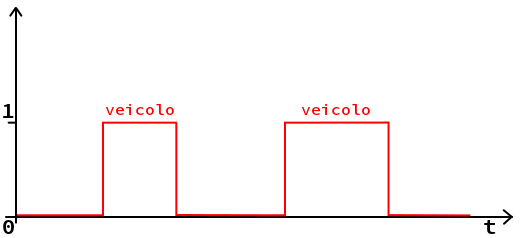
\includegraphics[width=1\columnwidth]{onda-quadra.png}
    \caption[Onda quadra]{Rappresentazione dell'onda quadra generata da un sensore a spira magnetica.}
    \label{fig:onda-quadra}
\end{figure}

Poiché \acs{TSIS} supporta esclusivamente la generazione di output aggregati rispetto al tempo (\eg{} densità dei veicoli per strada, velocità media, conteggio dei veicoli per sensore), si è reso necessario lo sviluppo di una \acl{RTE} dedicata che fosse in grado di memorizzare il dato atomico dei sensori al fine di ottenere la succitata \keyword{onda quadra} a tempo continuo.

In questo capitolo si presentano sia i succitati strumenti utilizzati per la creazione di reti stradali e relativi modelli di simulazione, sia l'estensione ideata per la creazione di dataset relativi al traffico.

Relativamente, invece, al processo pratico di creazione dei dataset si rimanda alla~\autoref{sec:create-dataset-howto}.

\cleardoublepage
\section{TSIS}
\label{sec:tsis}
\acf{TSIS} è un \acl{IDE}\footnote{Un \acl{IDE}, comunemente chiamato anche \ACF{IDE}, è un insieme di programmi finalizzati a supportare il processo di sviluppo dei software. Generalmente, un \acs{IDE} è costituito da uno strumento per la creazione e modifica del codice sorgente, un compilatore o un interprete, strumenti per l'automazione dello sviluppo e la qualità del codice sorgente.}, distribuito commercialmente da McTrans\footnote{McTrans Moving Technology: \url{http://mctrans.ce.ufl.edu}.} e supportato dalla \acf{FWHA}\footnote{Agenzia del Dipartimento dei Trasporti degli Stati Uniti d'America: \\ \url{www.fhwa.dot.gov}.}, il cui scopo ultimo è permettere la simulazione e l'analisi di modelli di reti stradali.

\acs{TSIS} è costituito da insieme di strumenti dedicati alla creazione di reti stradali e relativi modelli di simulazione, all'esecuzione, e eventualmente alla visualizzazione, di tali modelli, così come all'interpretazione dei risultati ottenuti. Tale insieme di strumenti è reso accessibile tramite delle interfaccie grafiche\footnote{Un'interfaccia grafica, nota anche come \acf{GUI}, è un tipo di interfaccia utente il cui fine è permettere all'utente di interagire con il software manipolando oggetti grafici convenzionali.}.

L'architettura modulare con cui \acs{TSIS} è realizzato permette, in caso di necessità, di estendere tale ambiente creando degli ulteriori strumenti.

Di seguito si introducono brevemente i concetti relativi a \acs{TSIS} utilizzati nel prosieguo di questo lavoro di tesi.

Tuttavia si osservi che, poiché lo scopo di questa sezione non consiste nel documentare \acs{TSIS}, la sua trattazione esaustiva (\eg{} semantica e lista completa dei tipi di dati rappresentabili) è omessa. A tale fine si rimanda invece alla documentazione ufficiale del software in questione.

\begin{definizione}[Progetto \acs{TSIS}]\label{defn:tsis-proj}
Un progetto \acs{TSIS} è un insieme di modelli di simulazione per una specifica rete stradale.
\end{definizione}

\begin{definizione}[Modello di simulazione \acs{TSIS}]\label{defn:tsis-sim-model}
Un modello di simulazione è costituito da un input (\eg{} variazioni dei flussi di ingresso nella rete, variazioni delle percentuali di svolta dei veicoli nelle intersezioni) per la simulazione di una determinata rete stradale e tutti i dati generati dalla sua esecuzione (\ie{} simulazione).
\end{definizione}
\begin{osservazione}
Un modello di simulazione può anche prevedere che la sua esecuzione sia eseguita più volte. Finché il seme dei numeri casuali non è modificato, esso è sempre considerato un singolo modello di simulazione.
\end{osservazione}

\begin{definizione}[Formato \acs{TRF}]\label{defn:trf-format}
\acs{TRF}\footnote{\acf{TRF}.} è il formato dei file accettati dal simulatore di \acs{TSIS}. Esso codifica e rappresenta una rete stradale e il relativo modello di simulazione specificandone i vari componenti tramite l'utilizzo dei rispettivi \acs{RT} (si veda la~\vref{defn:tsis-rt}).
\end{definizione}
\begin{osservazione}
Il formato \acs{TRF} è equivalente al formato \acs{TRAF}\footnote{\acf{TRAF}.}.
\end{osservazione}

\begin{definizione}[Formato \acs{TNO}]\label{defn:tno-format}
\acs{TNO}\footnote{\acf{TNO}.} è il formato nativo con cui vengono rappresentate in memoria le reti stradali create visivamente tramite l'interfaccia grafica \acs{TRAFED}.
\end{definizione}

\begin{definizione}[\acl{RT}]\label{defn:tsis-rt}
Un \acf{RT} rappresenta il blocco informativo minimo su cui è costruita una rete stradale e il suo modello di simulazione. Nel concreto esso consiste in una singola riga di testo nei file \acs{TRF} contenente un codice identificativo numerico e dei valori per i rispettivi campi accettati nell'ordine prestabilito. Allo stesso modo, tale formato descrive anche il modello di simulazione della rete stradale.
\end{definizione}

\begin{definizione}[\acs{RTE}]\label{defn:rte}
Una \ACF{RTE}, \acl{RTE}, è un'applicazione in grado di comunicare a tempo d'esecuzione con un'altra applicazione esterna. Una \acs{RTE}, in ambiente \emph{Microsoft Windows}, è solitamente compilata separatamente sotto forma di \acs{DLL}\footnote{Una \acf{DLL} è una libreria software che viene caricata dinamicamente in fase di esecuzione, invece di essere collegata staticamente a un eseguibile in fase di compilazione. Queste librerie sono anche chiamate \ACF{DLL}. L'acronimo \acs{DLL} corrisponde all'estensione che tali oggetti hanno in ambiente \emph{Microsoft Windows}. Tuttavia esse sono spesso chiamate più genericamente con il termine librerie condivise (da \emph{shared library}). Nei sistemi \emph{Linux}, esse sono anche note come oggetti \emph{shared object}.} e deve rispettare una determinata interfaccia: deve perciò implementare e esportare determinate funzioni che l'applicazione oggetto della comunicazione chiama a tempo d'esecuzione. Per la comunicazione in ingresso, invece, una \acs{RTE} deve essere collegata alle librerie dell'applicazione con cui intende interfacciarsi, avendo così accesso alle strutture dati e alle funzioni che questa esporta.
\end{definizione}

\subsection{Componenti}\label{subsec:tsis-components}
In questa sezione si elencano gli strumenti che costituiscono l'ambiente di sviluppo \acs{TSIS}.

\begin{description}
\item[CORSIM] \hfill \\
\acs{CORSIM}\footnote{\acf{CORSIM}.} costituisce il componente principale dell'insieme di strumenti denominato \acs{TSIS}. È un simulatore il cui obiettivo è permettere la creazione e l'esecuzione di modelli di simulazione \acs{TSIS}. È composto da due simulatori integrati che rappresentano l'intero sistema di traffico come funzione del tempo: \acs{NETSIM}\footnote{\acf{NETSIM}.} e \acs{FREESIM}\footnote{\acf{FREESIM}.}. Tali simulatori integrati rappresentano, rispettivamente, il traffico sulle strade urbane e non. La simulazione effettuata da tali strumenti è di tipo microscopico: essi modellano individualmente il comportamento di ogni singolo veicolo, prendendo in considerazione per ognuno di essi una serie di variabili, anche di tipo stocastico (\eg{} tipologia di guidatore). Per tale motivo \acs{CORSIM} è dotato di molte possibili opzioni di configurazione e permette lo studio di modelli molto complessi e dettagliati.
\item[TRAFED] \hfill \\
\acs{TRAFED}\footnote{\acf{TRAFED}.} è una \acs{GUI} il cui scopo è permettere la creazione e la modifica di reti stradali e di modelli di simulazione per \acs{CORSIM}.
\item[TShell] \hfill \\
\acs{TShell}\footnote{\acf{TShell}.} è la \acs{GUI} di \acs{TSIS}. Funge da contenitore degli strumenti (preconfigurati, o creati dall'utente) di questo ambiente di sviluppo integrato e permette la gestione dei progetti \acs{TSIS}.
\item[TRAFVU] \hfill \\
\acs{TRAFVU}\footnote{\acf{TRAFVU}.} è una \acs{GUI} finalizzata alla visualizzazione dei modelli di simulazione simulati con \acs{CORSIM}. Essa permette sia di visualizzare in modo animato l'evoluzione del traffico nella rete stradale con una qualsiasi granularità temporale, sia di visualizzare una serie di misure di interesse relative alla simulazione.
\item[TSIS Text Editor] \hfill \\
\acs{TSIS} \acsfont{Text Editor} è uno strumento il cui scopo è facilitare la modifica manuale dei file \acs{TRF}. A tale scopo esso visualizza per ogni \acs{RT} che si intende modificare sia la sua descrizione sia l'insieme dei campi supportati.
\item[TSIS Script Tool] \hfill \\
\acs{TSIS} \acsfont{Script Tool} è uno strumento per la creazione, la modifica e l'esecuzione di codice \acs{VBScript}\footnote{\acf{VBScript} è un linguaggio interpretato, sottoinsieme del linguaggio \emph{Visual Basic}, utilizzato come sostituto o integrazione della linea di comando o per il controllo di applicazioni esterne in ambiente \emph{Microsoft Windows}.}. Questo strumento fornisce un meccanismo utile ad automatizzare le funzionalità di simulazione di \acs{TSIS} (\eg{} esecuzioni multiple dello stesso modello di simulazione variando il seme dei numeri casuali che governa la distribuzione di ingresso dei veicoli nella rete stradale).
\item[TSIS Translator] \hfill \\
\acs{TSIS} \acsfont{Translator} è uno strumento utile alla conversione dei file dal formato \acs{TRF} al formato \acs{TNO} e viceversa. Tale operazione risulta utile al fine di rendere i file \acs{TRF} utilizzabili tramite lo strumento \acs{TRAFED} così come per rendere i file \acs{TNO} utilizzabili con \acs{CORSIM}.
\item[TSIS Output Processor] \hfill \\
\acs{TSIS} \acsfont{Output Processor} è uno strumento finalizzato alla raccolta e l'aggregazione dei dati da \acs{CORSIM} durante l'esecuzione multipla di modelli di simulazione. La sua caratteristica principale consiste nella computazione automatica di un insieme di statistiche predefinite. Esso permette di scegliere sia le statistiche di interesse sia la granularità temporale della loro computazione.
\end{description}

\subsection{Caratteristiche}\label{subsec:tsis-features}
Segue una panoramica il cui scopo è presentare sia le principali capacità, sia i vincoli di modellazione, simulazione e analisi di \acs{TSIS}.

\acs{TSIS}, tramite \acs{CORSIM}, permette la modellazione di reti stradali con le seguenti caratteristiche:

\begin{itemize}
    \item reti stradali urbane, non urbane o miste
    \item controllo quantitativo (\ie{} quantità di veicoli per intervallo temporale, distribuita secondo una distribuzione statistica) e qualitativo (\ie{} tipo di veicoli) dei flussi di veicoli in ingresso nella rete stradale
    \item controllo completo del flusso di traffico (\ie{} percentuali di svolta dei veicoli variabile nel tempo)
    \item supporto per strade con più corsie (massimo $9$)
    \item supporto dei segnali stradali
    \item supporto per gli attraversamenti pedonali
    \item intersezioni non controllate
    \item intersezioni controllate da semafori
    \item canalizzazione delle corsie
    \item piani semaforici predefiniti, dinamici (\eg{} priorità ai veicoli di emergenza) o guidati da algoritmi (\eg{} attivazione del semaforo in base alle rilevazioni effettuate dai sensori)
    \item sensori per la rilevazione del passaggio o della presenza di veicoli
    \item supporto per i mezzi di trasporto pubblico (\ie{} autobus, taxi)
    \item rilevamento di incidenti
    \item supporto per i sistemi di guida anglosassoni
    \item simulazione guidata all'analisi delle code
    \item simulazione guidata allo studio del grado di occupazione della rete stradale
    \item output di dati di interesse aggregati
    \item output di dati statistici collezionati
\end{itemize}

Poiché un modello di simulazione del traffico è caratterizzato dal cambiamento di un insieme di condizioni (\eg{} volumi di traffico, canalizzazione delle corsie, percentuali di svolta dei veicoli) della rete stradale, esso deve specificare, oltre alla natura stessa dei cambiamenti, anche i fattori in base a cui essi avvengono. Il fattore primario che viene preso in considerazione è il tempo. Ne consegue perciò che un modello di simulazione del traffico deve specificare l'intervallo temporale in cui specifici cambiamenti di determinate condizioni avvengono.

\acs{CORSIM} affronta questo problema permettendo di partizionare il tempo totale di simulazione in una serie di periodi temporali (\ie{} \emph{time period}) di durata variabile. Ogni periodo temporale possiede perciò un insieme di dati di input che non variano per tutta la sua durata. Inoltre, i periodi temporali sono a loro volta suddivisi in intervalli temporali (\ie{} \emph{time interval}), anch'essi suddivisi in passi temporali (\ie{} \emph{time step}).

Le principali limitazioni di \acs{TSIS} derivano dalle modalità con cui \acs{CORSIM} implementa la gestione del tempo: la lista dei periodi temporali è rappresentata internamente tramite un array statico di dimensione prefissata. Nello specifico, un modello \acs{CORSIM} può essere costituito da un massimo di $19$ periodi temporali, ognuno dei quali viene specificato tramite il \acs{RT} $03$, e può avere una durata compresa tra i $10$ e i $9999$ secondi. Ognuno di tali periodi temporali è suddiviso in intervalli (specificati tramite dei \acs{RT} $04$) la cui durata, compresa tra $1$ e $200$ secondi, deve essere un sottomultiplo della durata del periodo temporale cui appartiene. Infine, ogni intervallo temporale è partizionato in passi temporali: \acs{NETSIM} utilizza un passo temporale fisso di $1$ secondo mentre \acs{FREESIM} opera in base al passo temporale specificato dall'utente. Poiché i due modelli di simulazione microscopica che costituiscono \acs{CORSIM} operano in modo sincronizzato, la durata del passo temporale di \acs{FREESIM}, anche se compresa nell'intervallo $[0.1,1]$ secondi, non può essere specificata liberamente dall'utente. All'utente è permesso specificare solo il numero di passi temporali di \acs{FREESIM} (tramite il campo $1$, \acs{RT} $04$) che devono essere eseguiti per ogni secondo di simulazione. Tale approccio permette perciò di utilizzare dei passi temporali di durata minore per il simulatore \acs{FREESIM} mantenendo la sincronizzazione con il simulatore \acs{NETSIM}.

La~\vref{tab:fresim-time-steps} mostra la corrispondenza tra il numero di passi temporali di \acs{FREESIM} e la reale durata che verrà loro assegnata.
\begin{table}[h]%
    \centering%
    \begin{tabular}{+c^c}
    \toprule\rowstyle{\bfseries}%
    Valore del campo $1$    & Durata del passo temporale in \acs{FREESIM}   \\
                            & (sec)                                         \\\otoprule%
    1                       & 1.0                                           \\
    2                       & 0.5                                           \\
    3                       & 0.333333                                      \\
    4                       & 0.25                                          \\
    5                       & 0.2                                           \\
    6                       & 0.166667                                      \\
    7                       & 0.142857                                      \\
    8                       & 0.125                                         \\
    9                       & 0.111111                                      \\
    10                      & 0.1                                           \\\bottomrule
    \end{tabular}
    \caption[Durata dei passi temporali in \acs{FREESIM}]{Relazione tra numero di passi temporali per ogni secondo di simulazione e durata effettiva del passo temporale in \acs{FREESIM}.}
    \label{tab:fresim-time-steps}
\end{table}

La~\vref{fig:corsim-time} mostra, tramite un esempio, quanto appena descritto relativamente alla rappresentazione del tempo in \acs{CORSIM}.

Si osservi, inoltre, che la granularità temporale massima con cui è possibile ottenere statistiche cumulative, e, in generale, dati relativi alla simulazione, corrisponde alla durata scelta per gli intervalli temporali (si veda a tal riguarda la documentazione relativa al tipo \acs{RT} $05$). Si consideri ad esempio la~\vref{fig:corsim-time}: in tal caso non sarà possibile ottenere dati cumulati relativi a un intervallo di tempo minore di $60$ secondi.
\begin{figure}[htbp]
    \centering
    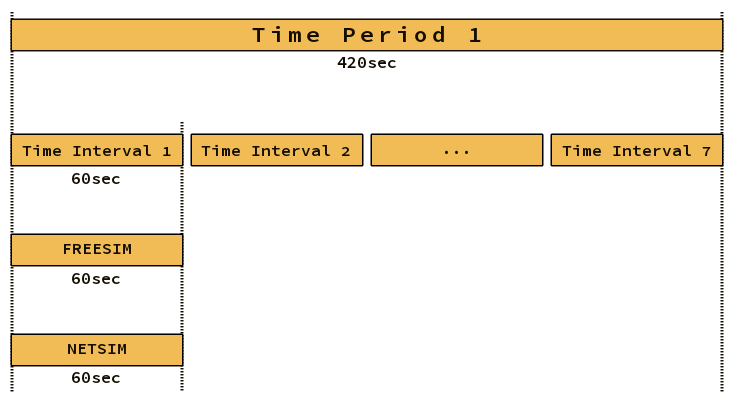
\includegraphics[width=1\columnwidth]{corsim-time}
    \caption[Gestione del tempo in \acs{CORSIM}]{Esempio di suddivisione gerarchica delle unità temporali in \acs{CORSIM}. Un \emph{time period} della durata di $420$ secondi è suddiviso in $7$ \emph{time interval}, ciascuno della durata di $60$ secondi. Ogni \emph{time interval} verrà poi automaticamente diviso in $60$ \emph{time step} da $1$ secondo ciascuno per \acs{NETSIM} (\ie{} linee rosse). La durata di tali \emph{time step} di \acs{NETSIM} può o meno coincidere, come accade in questo esempio, con quella assegnata ai \emph{time step} di \acs{FREESIM} a seconda del valore del campo $1$ del \acs{RT} $04$ nel modello \acs{CORSIM}.}
    \label{fig:corsim-time}
\end{figure}

La gestione del tempo che \acs{CORSIM} attua implica quindi alcune limitazioni:
\begin{itemize}
    \item il tempo massimo di simulazione, benché sufficiente nella maggior parte dei casi, è di circa $52$ ore
    \item la massima granularità con cui è possibile raccogliere informazioni è di $1$ secondo, impostando a tale valore la durata degli intervalli temporali
    \item i dati raccolti dalla simulazione sono sempre aggregati in base alla durata dell'intervallo temporale cui si riferiscono.
\end{itemize}
Tali vincoli rendono impossibile recuperare l'output dei sensori a tempo continuo in modo non aggregato o in generale con una granularità temporale inferiore a $1$ secondo. Al fine di sorpassare tali limitazioni si è proceduto sviluppando una \acl{RTE} apposita, \acsfont{Sensors} \acs{DLL}, descritta dettagliatamente nella \vref{sec:sensors-rte}. Al fine di rendere la descrizione di tale software maggiormente chiara, è necessario presentare il meccanismo di estensione di \acs{CORSIM}. La sezione che segue affronta perciò tale argomento.

\section{Creazione di estensioni TSIS}
\acs{TSIS} espone un meccanismo finalizzato all'estensione delle sue funzionalità tramite la creazione, da parte dell'utente, di altri strumenti da integrare nell'ambiente di sviluppo. Tali strumenti, interfacciandosi direttamente con \acs{CORSIM}, possono modificarne o aumentarne la logica di simulazione, collezionare dati o monitorare eventi speciali (\eg{} indicenti).

In questa sottosezione si presenta il funzionamento dei meccanismi di interfacciamento (\ie{} più brevemente detti \acs{API}\footnote{Con il termine
\acf{API} si indica un insieme di procedure rese disponibili all'esterno, di solito raggruppate a formare un insieme di strumenti specifici per l'espletamento di un determinato compito all'interno di un programma.}) tra \acs{CORSIM} e strumenti esterni, a cui ci si riferirà da questo momento in poi con il termine \acs{CORSIM} \acs{RTE}.

\subsection{Requisiti}
Al fine di sviluppare e compilare con successo una \acs{CORSIM} \acs{RTE} in \CC{} è necessario disporre dei seguenti strumenti:
\begin{itemize}
    \item il compilatore della piattaforma \emph{Microsoft Visual \CC{}}
    \item il pacchetto software di \acs{TSIS}, il quale include di default tutti i componenti necessari mostrati dalla~\vref{fig:tsis-corsim-arch} (ad eccezione, chiaramente, del componente \acs{RTE}).
\end{itemize}
Si osservi, inoltre, che è possibile sviluppare una \acs{CORSIM} \acs{RTE} anche in linguaggio \lstinline[]|C| o \lstinline[]|FORTRAN|.

\subsection{Architettura di CORSIM}

La~\vref{fig:tsis-corsim-arch} illustra l'architettura modulare di \acs{CORSIM} e il suo funzionamento all'interno dell'ambiente di sviluppo \acs{TSIS}.
\begin{figure}
    \centering
    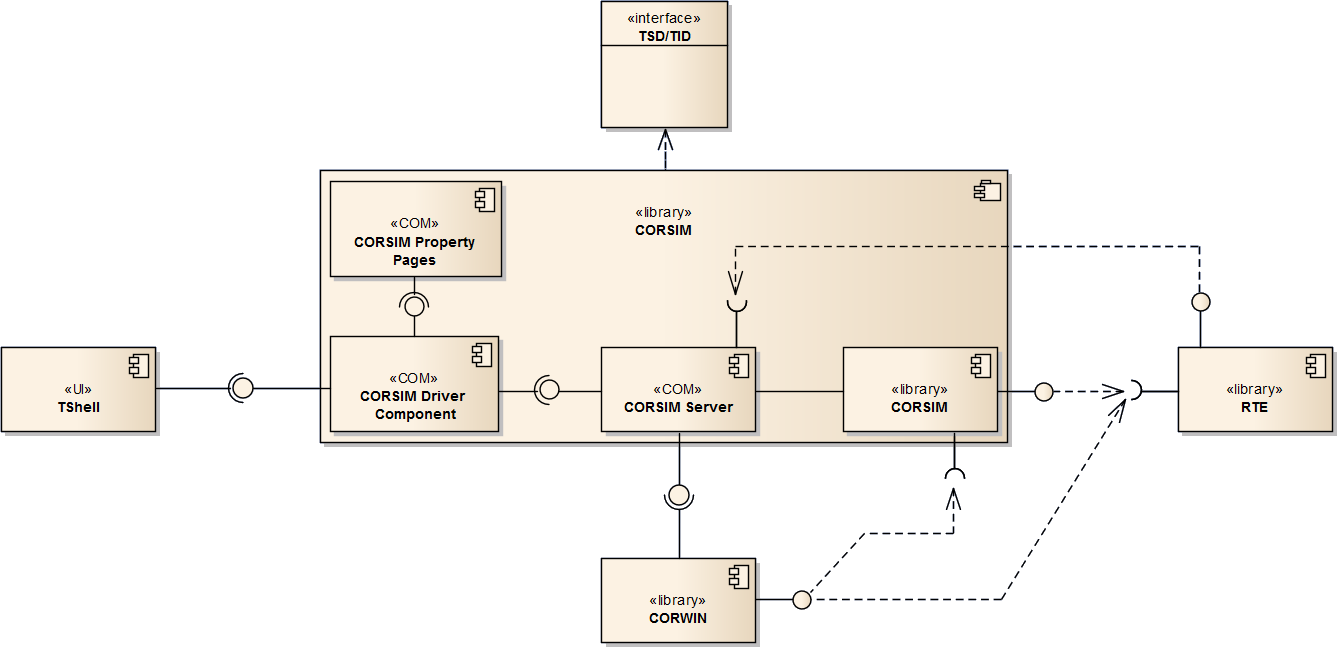
\includegraphics[width=0.925\columnwidth]{tsis-corsim-components}
    \caption[Diagramma dei componenti di \acs{CORSIM}]{Porzione del diagramma dei componenti di \acs{TSIS}: mostra l'architettura modulare e il funzionamento di \acs{CORSIM} all'interno di \acs{TSIS}.}
    \label{fig:tsis-corsim-arch}
\end{figure}
Si osservi che i componenti che costituiscono \acs{CORSIM} sono di due tipi: librerie \acs{DLL} e moduli \acs{COM}\footnote{Il \acf{COM} è uno standard per componenti software ideato da \emph{Microsoft}. Il suo fine consiste nel permettere la comunicazione fra processi e la creazione dinamica di oggetti. Una interfaccia \acs{COM} è una collezione di funzioni, incapsulata in un componente software binario e neutrale rispetto al linguaggio.}. Il \acs{CORSIM} \acsfont{Driver Component}, ad esempio, è il modulo \acs{COM} di \acs{TSIS} preposto a interfacciare \acs{CORSIM} e \acs{TShell}, permettendo così il controllo e l'esecuzione di \acs{CORSIM}, delle \acs{RTE} create dall'utente e degli altri strumenti (\eg{} \acs{TSIS} \acsfont{Output Processor}) di \acs{TSIS} tramite \acs{GUI}.

Anche se la~\vref{fig:tsis-corsim-arch} mostra per completezza l'intera architettura di \acs{CORSIM}, si procede con la descrizione delle interfacce di \acs{CORSIM} preposte alla comunicazione con \acs{RTE} sviluppate dall'utente, identificate dalle frecce tratteggiate e numerate.

Per ogni passo temporale di simulazione, il \acs{CORSIM} \acsfont{Server} chiama una serie di funzioni di \acs{CORSIM} finalizzate a guidare l'andamento della simulazione. Quando una \acs{RTE} viene inserita nell'ambiente di sviluppo integrato, il \acs{CORSIM} \acsfont{Server} chiama anche le funzioni che la \acs{RTE} esporta in base ai messaggi che riceve da \acs{CORSIM} durante la sua esecuzione. Questa interfaccia è rappresentata dalla freccia $1$ nella~\vref{fig:tsis-corsim-arch}; la~\autoref{subsec:corsim-lifecycle} \vpageref{subsec:corsim-lifecycle} riporta maggiori dettagli sui punti di chiamata che \acs{CORSIM} espone.

\acs{TSIS} fornisce inoltre una \acs{API}, identificata dalla freccia $2$ nella~\vref{fig:tsis-corsim-arch}, chiamata \acsfont{CORWIN}, che permette alle \acs{RTE} di inviare messaggi al modulo \acs{CORSIM} \acsfont{Server} affinché essi siano visualizzati in \acs{TShell} dal \acs{CORSIM} \acsfont{Driver Component}.

Infine, una \acs{RTE} può accedere direttamente a una serie di funzioni e strutture dati esportate da \acs{CORSIM} nella memoria condivisa. Anche se non è possibile riferirsi a questo meccanismo di comunicazione come una \acs{API} vera e propria, nel prosieguo, ci riferiremo ad essa con il termine \acs{CORSIM} \acs{API} al fine di semplificare la discussione. Perciò, la \acs{CORSIM} \acs{API}, rappresentata dalla freccia $3$ della~\vref{fig:tsis-corsim-arch}, oltre a permettere l'estrazione di informazioni relative alla simulazione, permette alla \acs{RTE} di controllare, eventualmente, molti aspetti della simulazione operata da \acs{CORSIM} (\eg{} aborto della simulazione).

Si osservi che, anche se la~\vref{fig:tsis-corsim-arch} non evidenzia tale possibilità, l'architettura di \acs{CORSIM} supporta l'utilizzo di più \acs{RTE} contemporaneamente.

\begin{nota}
Un attento osservatore noterà come \acs{CORSIM}, la libreria finalizzata al processo di simulazione, sia a sua volta una \acs{RTE} automaticamente collegata ai moduli \acs{CORSIM} \acsfont{Server} e \acsfont{CORWIN}. Inoltre, la~\vref{fig:tshell-tool-config-1} fa notare come tutti i componenti (elencati e descritti nella~\autoref{subsec:tsis-components} \vpageref{subsec:tsis-components}) dell'ambiente di sviluppo \acs{TSIS} siano anch'essi dei moduli architetturalmente uguali alle \acs{RTE}.
\end{nota}

\subsection{Ciclo di vita di CORSIM}\label{subsec:corsim-lifecycle}
Di seguito si presenta il ciclo di vita di \acs{CORSIM} descrivendo i punti di chiamata che esso esporta tramite apposite funzioni affinché una \acs{RTE}, implementando ed esportando una funzione per almeno uno di essi, possa interfacciarsi con il processo di simulazione. Tali informazioni sono quindi relative alla \acs{API} rappresentata dalla freccia $1$ nella~\vref{fig:tsis-corsim-arch}. Le modalità di implementazione e utilizzo in \CC{} di tale \acs{API} sono illustrate nella~\autoref{subsec:tsis-api-examples} \vpageref{subsec:tsis-api-examples}.

La~\vref{tab:corsim-lifecycle} descrive tutti i punti di chiamata relativi alla linea di esecuzione temporale di \acs{CORSIM}.
\begin{table}[ht]%
    \begin{tabularx}{\columnwidth}{+l^X}
    \toprule\rowstyle{\bfseries}%
    Punto di chiamata                   & Descrizione                                   \\
    \otoprule%
    \lstinline[]|Initialize|            & \small Chiamato all'inizio della simulazione prima della fase di inizializzazione \acs{CORSIM} ma dopo la lettura del file \acs{TRF} di input.                                                            \\
    \lstinline[]|PostVehicleEmit|       & \small Chiamato ad ogni \emph{time step} dopo che i veicoli sono stati immessi nella rete stradale.                                                                           \\
    \lstinline[]|PreNetsimVehicle|      & \small Chiamato ad ogni \emph{time step} appena prima che i veicoli inizino a muoversi nel sotto-modello \acs{NETSIM}.                                                                                   \\
    \lstinline[]|PreNetsimSignal|       & \small Chiamato ad ogni \emph{time step} appena prima che i segnali (\eg{} semafori) del sotto-modello \acs{NETSIM} vengano impostati.                                                                  \\
    \lstinline[]|PostNetsimTimestep|    & \small Chiamato in corrispondenza della fine del processo di simulazione di ogni \emph{time step} di \acs{NETSIM} e prima che \acs{FREESIM} inizi a simulare il suo relativo sotto-modello.                   \\
    \lstinline[]|PreFresimVehicle|      & \small Chiamato ad ogni \emph{time step} appena prima che i veicoli inizino a muoversi nel sotto-modello \acs{FREESIM}.                                                                                   \\
    \lstinline[]|PreFresimSignal|       & \small Chiamato ad ogni \emph{time step} appena prima che i segnali (\eg{} semafori) del sotto-modello \acs{FREESIM} vengano impostati.                                                                  \\
    \lstinline[]|PostFresimTimestep|    & \small Chiamato in corrispondenza della fine del processo di simulazione di ogni \emph{time step} di \acs{FREESIM}.
                                                                                        \\
    \lstinline[]|BeginSimulation|       & \small Chiamato dopo l'inizializzazione di \acs{CORSIM} (\ie{} rete stradale piena) in corrispondenza dell'inizio della simulazione.                                                                        \\
    \lstinline[]|TimeStepComplete|      & \small Chiamato in corrispondenza della fine del processo di simulazione di ogni \emph{time step}.                                                                                   \\
    \lstinline[]|TimeIntervalComplete|  & \small Chiamato in corrispondenza della fine del processo di simulazione di ogni \emph{time interval}.                                                                                   \\
    \lstinline[]|TimePeriodComplete|    & \small Chiamato in corrispondenza della fine del processo di simulazione di ogni \emph{time period}.                                                                                   \\
    \lstinline[]|TimePeriodValidated|   & \small Chiamato in corrispondenza della fine del processo di lettura e validazione del file di input relativo a ogni \emph{time period}, prima dell'inizializzazione e dell'effettivo inizio del processo di simulazione di ogni \emph{time period}.                                                                                   \\
    \lstinline[]|SimulationComplete|    & \small Chiamato in corrispondenza della fine della simulazione e prima della completa terminazione del processo.                                                                           \\
    \lstinline[]|Shutdown|              & \small Chiamato appena prima che l'esecuzione di \acs{CORSIM} termini.
                                                                                        \\
    \lstinline[]|Exit|                  & \small Chiamato in corrispondenza della fine dell'intero processo di simulazione.
                                                                                        \\\bottomrule
    \end{tabularx}
    \caption[Ciclo di vita di \acs{CORSIM}]{Descrizione di punti di chiamata che \acs{CORSIM} espone all'esterno.}
    \label{tab:corsim-lifecycle}
\end{table}
Una volta compilata la \acs{RTE} e ottenuto il relativo file \acs{DLL}, ognuno dei punti di chiamata di \acs{CORSIM} deve essere associato alla rispettiva funzione implementata dalla \acs{RTE}. La sezione che segue descrive in maggior dettaglio tale processo.

\subsection{Collegare una RTE a CORSIM}\label{subsec:rte-corsim-linking}
Questa sottosezione illustra i passi necessari a espletare il processo di collegamento (\ie{} \emph{linking}) di una \acs{RTE} a \acs{CORSIM}. Tale processo è eseguibile direttamente tramite \acs{TShell}.

A scopo esemplificativo si descrive come aggiungere la \acs{RTE} per il rilevamento e tracciamento del passaggio dei veicoli sui sensori (descritta nella~\vref{sec:sensors-rte}). Tale operazione viene svolta tramite il menù \emph{Tools} di \acs{TShell} scegliendo la voce \emph{Tool Configuration} e cliccando sul pulsante per l'aggiunta (\ie{} \emph{Add}) di una \acs{RTE}. La~\vref{fig:tshell-tool-config-1} mostra lo strumento di configurazione degli strumenti appartenenti all'ambiente di \acs{TSIS}.

\begin{figure}[H]
    \centering
    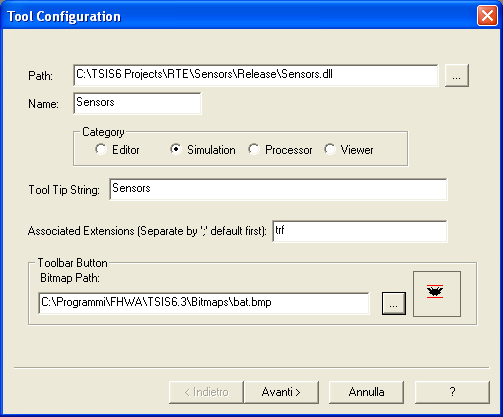
\includegraphics[width=1\columnwidth]{tshell-tool-config-1}
    \caption[Aggiunta di una \acs{RTE} a \acs{TSIS}]{Strumento finalizzato all'aggiunta di una \acs{RTE} a \acs{TSIS}.}
    \label{fig:tshell-tool-config-1}
    \end{figure}
    Specificato il percorso a cui risiede il file \acs{DLL} della \acs{RTE}, il tipo di \acs{RTE}, il nome e l'icona che si intende assegnare a tale strumento e il tipo di file a cui va associato (\eg{} \acs{TRF}), la \acs{RTE} è aggiunta a \acs{TSIS}. La~\vref{fig:tshell-toolbar} mostra la barra degli strumenti di \acs{TShell} quando un file \acs{TRF} viene aperto: essa contiene il pulsante per l'avvio della \acs{RTE} appena aggiunta all'ambiente di sviluppo \acs{TSIS}.
    \begin{figure}[H]
    \centering
    
\includegraphics[width=0.4\columnwidth]{tshell-toolbar}
    \caption[Barra degli strumenti di \acs{TShell}]{Barra degli strumenti di \acs{TShell} contenente il pulsante per l'invocazione della \acs{RTE} aggiunta all'ambiente di sviluppo \acs{TSIS}.}
    \label{fig:tshell-toolbar}
\end{figure}

Tuttavia, come detto, le funzioni della \acs{RTE} devono essere collegate ai punti di chiamata di \acs{CORSIM} affinché la \acs{RTE} risulti completamente funzionante. Per adempiere tale operazione è necessario utilizzare nuovamente lo strumento di configurazione cliccando sul pulsante per la modifica (\ie{} \emph{Edit}) di una \acs{RTE}. A questo punto, selezionando la scheda relativa alle \acs{RTE}, è possibile invocare lo strumento per effettuare il succitato collegamento. La~\vref{fig:tshell-tool-config-8} mostra il processo di collegamento tra le funzioni della \acs{RTE} e i punti di chiamata di \acs{CORSIM}.
\begin{figure}[H]
    \centering
    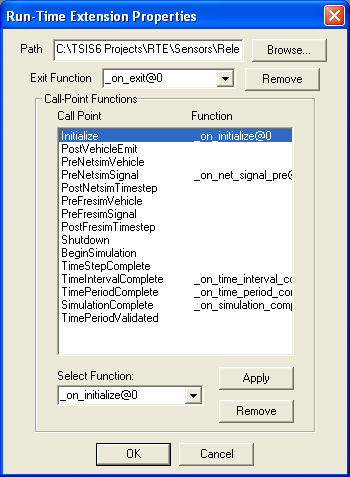
\includegraphics[width=1\columnwidth]{tshell-tool-config-8}
    \caption[Collegamento delle funzioni della \acs{RTE} a \acs{CORSIM}]{Collegamento delle funzioni della \acs{RTE} ai rispettivi punti di chiamata di \acs{CORSIM}.}
    \label{fig:tshell-tool-config-8}
\end{figure}

Inoltre, può essere necessario dover configurare la \acs{RTE} aggiunta in base alle sue esigenze, così come modificare alcune funzionalità di \acs{CORSIM} relativamente ad essa. Ad esempio, la \acs{RTE} per il monitoraggio e il tracciamento del passaggio dei veicoli sui sensori non necessita che i file di output di \acs{CORSIM} vengano generati, né che vengano generati i file per la visualizzazione animata della simulazione in \acs{TRAFED}. Inoltre, tale \acs{RTE}, non necessita che la simulazione \acs{CORSIM} sia eseguita più volte. La~\vref{fig:tshell-tool-config-35} mostra la configurazione di tali opzioni.
\begin{figure}[H]
    \centering
    \subfloat[Proprietà di \acs{CORSIM}.]
    {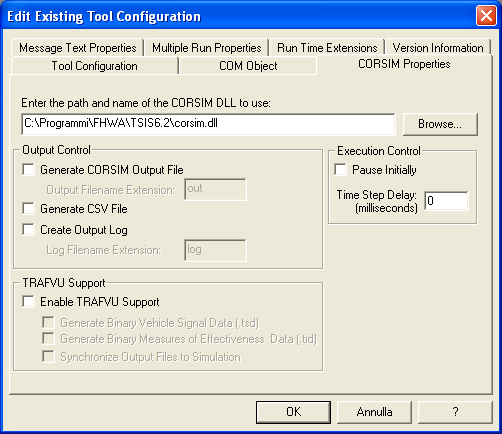
\includegraphics[width=1\columnwidth]{tshell-tool-config-3}} \\
    \subfloat[Impostazioni proprietà d'esecuzione di \acs{CORSIM}.]
    {\label{fig:ipsum}%
    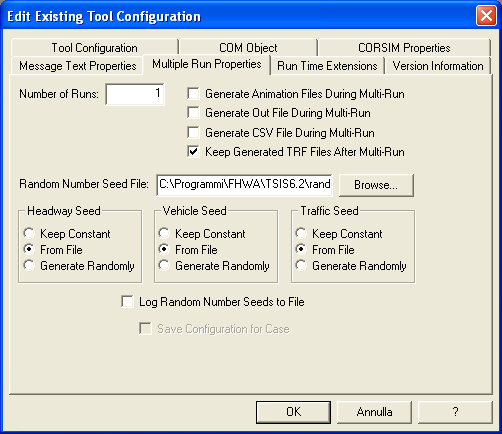
\includegraphics[width=1\columnwidth]{tshell-tool-config-5}}
    \caption[Configurazione delle proprietà di \acs{CORSIM}]{Configurazione delle proprietà di \acs{CORSIM} per la \acs{RTE}: disattivazione dell'output di \acs{CORSIM}, della generazione dell'input per \acs{TRAFED} e delle esecuzioni multiple della simulazione.}
    \label{fig:tshell-tool-config-35}
\end{figure}

\cleardoublepage
\subsection{Utilizzo delle API}\label{subsec:tsis-api-examples}
Lungi dal volere fornire una documentazione esaustiva delle \acs{API} dell'ambiente di sviluppo \acs{TSIS}, in questa sezione, si intende presentare, tramite esempi, le modalità di utilizzo di tali \acs{API} in linguaggio \CC{}.

Ad esempio, il listato~\ref{lst:callpoint-api} mostra il codice di intestazione necessario a definire ed esportare la funzione \lstinline[]|on_initialize| (listato~\ref{lst:callpoint-impl}), che, come mostrato dalla~\vref{fig:tshell-tool-config-8} viene collegata al punto di chiamata \lstinline[]|Initialize| di \acs{CORSIM}. Si osservi che la scelta del nome di tale funzione non è vincolata ad alcun criterio.

\vspace*{8pt}\inputsourcecode[language=cpp,caption={Costrutto per l'esportazione delle funzioni \acs{RTE}}, label=lst:callpoint-api]{codes/callpointapi}

\inputsourcecode[language=cpp,caption={Esempio di funzione \acs{RTE} esportata}, label=lst:callpoint-impl]{codes/callpointimpl}

Il listato~\ref{lst:corwin-api} illustra invece come importare una delle funzioni esposte dalla \acsfont{CORWIM} \acs{API} in una \acs{RTE}. Nello specifico, l'esempio in questione, è relativo all'importazione della funzione \lstinline[]|OutputString|, finalizzata all'invio di messaggi di output a \acs{TShell} durante la simulazione \acs{CORSIM}.

\vspace*{8pt}\inputsourcecode[language=cpp, caption=Importazione delle \acsfont{CORWIN} \acs{API}, label=lst:corwin-api]{codes/corwinapi}

Infine, come già detto, \acs{CORSIM} permette l'accesso alla maggior parte dei dati che esso manipola durante la simulazione, esportandoli nella memoria condivisa. Tali dati sono dei seguenti tipi:
\begin{enumerate}
    \item variabili scalari (non array)
    \item array allocati staticamente
    \item array allocati dinamicamente
    \item funzioni esposte tramite \acs{API}.
\end{enumerate}

Il listato~\ref{lst:corsim-api-dll-import} mostra il costrutto utilizzabile per l'importazione di dati e funzioni dalla cosiddetta \acs{CORSIM} \acs{API}.
\vspace*{8pt}\inputsourcecode[language=cpp, caption=Costrutto per l'importazione delle \acs{CORSIM} \acs{API}, label=lst:corsim-api-dll-import]{codes/corsimapidllimport}

Tale costrutto viene poi utilizzato per l'effettiva importazione di dati e funzioni da \acs{CORSIM}. Il listato~\ref{lst:corsim-api} riporta un esempio di importazione per ogni tipo di dati che le \acs{CORSIM} \acs{API} rendono disponibile:
\begin{enumerate}
    \item a~\autoref{lst:netsim-num-dets-import} si importa il numero di sensori presenti sulla rete stradale urbana, esportato da \acs{CORSIM} tramite la variabile scalare \lstinline[]|NETSIM_DETECTORS_mp_NUMDET| e rinominato, a~\autoref{lst:netsim-num-dets-assign}, in \lstinline[]|net_det_num|
    \item a~\autoref{lst:netsim-nmap-import} si importa la lista statica (\ie{} di dimensione massima prefissata) dei numeri identificativi assegnati dall'utente ai nodi della rete stradale, \lstinline[]|SIN075.NMAP|; rinominata a~\autoref{lst:netsim-nmap-assign} in \lstinline[]|net_node_num|
    \item a~\autoref{lst:netsim-dets-mod-import} si importa la lista dinamica delle informazioni sui sensori, \lstinline[]|*NETSIM_DETECTORS_mp_DETMOD|; rinominata, a~\autoref{lst:netsim-dets-mod-assign}, in \lstinline[]|net_det_mod|
    \item a~\autoref{lst:netsim-abort-func-import} si importa \lstinline[]|abortcorsim|, una funzione delle \acs{CORSIM} \acs{API} finalizzata al controllo dell'esecuzione della simulazione da parte della \acs{RTE}
\end{enumerate}

\vspace*{8pt}\inputsourcecode[language=cpp, caption=Importazione di oggetti delle \acs{CORSIM} \acs{API}, label=lst:corsim-api]{codes/corsimapi}

\cleardoublepage
\section{Estensione}\label{sec:sensors-rte}
Avendo presentato l'ambiente di sviluppo \acs{TSIS} e le \acs{API} che esso fornisce per la sua estensione, è ora possibile descrivere l'\acl{RTE} sviluppata al fine di generare i succitati dataset.

Come detto nella~\autoref{subsec:tsis-features} \vpageref{subsec:tsis-features}, una delle principali limitazioni di \acs{CORSIM} consiste nell'impossibilità di ottenere dei dati non aggregati dal processo di simulazione. Ciò poiché il minimo intervallo temporale che \acs{CORSIM} permette di utilizzare è pari a $1$ secondo per le reti stradali urbane e al più $0.1$ secondi per le reti stradali extraurbane. Perciò, è emerso il problema di sorpassare tale limitazione. La \acs{RTE} sviluppata, \acsfont{Sensors} \acs{DLL}, risponde a tale necessità monitorando determinati elementi (\ie{} i sensori) di un qualsiasi tipo di rete stradale e tracciando gli eventi ad essi correlati (\ie{} passaggio di un veicolo) su un file di output esterno a \acs{TSIS}. Lo scopo di questa sezione consiste nel presentare il funzionamento di \acsfont{Sensors} \acs{DLL}.

\subsection{Sensors DLL}\label{subsec:sensors-dll}
L'obiettivo ultimo di \acsfont{Sensors} \acs{DLL} consiste nella generazione di un file \acs{CSV}\footnote{\acf{CSV} è un formato basato su file di testo utilizzato per l'importazione ed esportazione (ad esempio da fogli elettronici o database) di una tabella di dati.} che rappresenti il passaggio dei veicoli sui vari sensori presenti nella rete stradale nel tempo. Il monitoraggio dei sensori deve essere effettuato con la massima granularità temporale possibile (\ie{} $0.1$ secondi), anche nel caso di reti stradali urbane.

A tale scopo si è utilizzato il dato \lstinline[]|NETSIM_DETECTORS_mp_DETON|, rinominato in \lstinline[]|net_det_on|, esportato da \acs{CORSIM} nella memoria condivisa. Tale campo indirizza un array dinamico la cui lunghezza è pari al numero di sensori sulla rete stradale. Ognuno degli elementi di tale array è costituito da $10$ bit: l'$i$-esimo bit rappresenta l'attivazione (\ie{} $1$) o meno del relativo sensore nell'$i$-esimo passo temporale minimo (\ie{} $0.1$ secondi). Ogni elemento rappresenta perciò il passaggio dei veicoli sul sensore durante un intervallo temporale fisso di $1$ secondo.

Di seguito si presentano le operazioni principali che \acsfont{Sensors} \acs{DLL} effettua:
\begin{enumerate}
    \item ottenere il nome del file \acs{TRF} di input, rappresentante la rete stradale e il modello di simulazione
    \item effettuare il \emph{parsing}\footnote{Il \emph{parsing} consiste nel processo atto ad analizzare un input in modo da determinare la sua struttura grammaticale grazie ad una data grammatica formale.} di tale file creando gli oggetti relativi a ogni elemento (\eg{} intersezioni, strade, sensori) della rete stradale
    \item rilevare il passaggio dei veicoli sui sensori ogni secondo
    \item ricostruire l'intero flusso di veicoli su ogni sensore durante tutto il tempo di simulazione
    \item creare un file di output che contenga le informazioni ottenute.
\end{enumerate}
Le operazioni $1$ e $2$ vengono compiute in corrispondenza dell'inizializzazione di \acs{CORSIM} e quindi della \acs{RTE}. Il risultato di tali operazioni è un insieme di istanze correlate rappresentanti gli elementi della rete stradale di input e le caratteristiche di ognuno di essi. Il diagramma delle classi di \acsfont{Sensors} \acs{DLL}, mostrato in~\vref{fig:sensors-class-diagram}, illustra le relazioni di associazione e aggregazione degli oggetti con cui si è scelto di rappresentare le reti stradali \acs{TSIS}. La classe \lstinline[]|CNetwork| rappresenta la rete stradale, composta da un insieme di intersezioni e strade, elementi rappresentati rispettivamente dalle classi \lstinline[]|CNode| e \lstinline[]|CLink|. Ogni strada può a sua volta essere composta da più corsie, elementi rappresentati tramite la classe \lstinline[]|CLane|, e contenere dei sensori, elementi rappresentati tramite la classe \lstinline[]|CDetector|. Inoltre, poiché è possibile che alcuni sensori siano posti esclusivamente su una corsia piuttosto che su tutta la superficie della strada, sussiste una relazione anche fra la classe rappresentante le corsie e quella rappresentante i sensori. Invece, la classe \lstinline[]|CBinary| non rappresenta alcun elemento concreto della rete stradale: la sua funzione è esclusivamente quella di incapsulare l'intero \lstinline[]|net_det_on| e convertirlo nella corretta sequenza di bit rappresentante il flusso dei veicoli su un sensore. La procedura che effettua tali operazioni di inizializzazione della rete stradale nella \acs{RTE}, chiamata \lstinline[]|on_initialize|, è collegata al punto di chiamata \lstinline[]|Initialize|, così come mostrato dalla~\vref{fig:tshell-tool-config-8}.

Configurata la rete stradale, \acsfont{Sensors} \acs{DLL} può monitorare i sensori di pari passo con l'esecuzione della simulazione da parte di \acs{CORSIM}. Tale operazione viene effettuata ad ogni intervallo temporale di \acs{NETSIM} poiché la procedura che la incorpora, chiamata \lstinline[]|on_net_signal_pre|, è collegata al punto di chiamata \lstinline[]|PreNetsimSignal| di \acs{CORSIM}. Il listato~\ref{lst:process-sensors} a pagina~\pageref{lst:process-sensors} illustra una versione semplificata del metodo \CC{} preposto all'esecuzione di tale procedura. Essa consiste nell'iterazione della lista di sensori afferenti ad una strada: per ogni sensore (ciclo a~\autoref{lst:iterate-sensors}), recuperato l'identificatore che \acs{CORSIM} utilizza per rappresentarlo (istruzione a~\autoref{lst:get-sensor-id}), si ottiene il relativo elemento dell'array \lstinline[]|net_det_on| (istruzione a~\autoref{lst:get-sensor-on}), un intero rappresentante il flusso di veicoli sul sensore nell'ultimo secondo di simulazione. Tale intero viene poi convertito nella corretta sequenza di $10$ bit tramite la classe \lstinline[]|CBinary| a~\autoref{lst:get-sensor-bits}. Da~\autoref{lst:get-sensor-state-start} a~\autoref{lst:get-sensor-state-end} si itera in ordine inverso la sequenza di bit al fine di estrapolare e memorizzare lo stato (\ie{} $1$ in caso di veicolo rilevato, $0$ altrimenti) del sensore in ogni passo temporale minimo (\ie{} $0.1$ secondi). Quindi questa procedura, ripetuta per tutte le strade presenti nella rete stradale e ad ogni intervallo temporale, memorizza per ogni sensore una lista di valori booleani.

Completata la simulazione e di conseguenza anche la procedura di monitoraggio dei sensori, \acsfont{Sensors} \acs{DLL}, in corrispondenza del punto di chiamata \lstinline[]|SimulationComplete| di \acs{CORSIM}, genera un file \acs{CSV} in cui memorizza il tempo, il \emph{time period} della rilevazione e la dinamica di stato di ogni sensore. La~\autoref{subsec:sensors-dll-output} \vpageref{subsec:sensors-dll-output} si occupa di presentare in maggior dettaglio l'output di \acsfont{Sensors} \acs{DLL}.

\vspace*{8pt}\inputsourcecode[caption={[Rilevazione del passaggio dei veicoli sui sensori]Metodo della classe \lstinline[]|CLink| per la rilevazione del passaggio dei veicoli sui sensori}, label=lst:process-sensors, language=cpp]{codes/processsensors}

\begin{figure}[H]
    \centering
    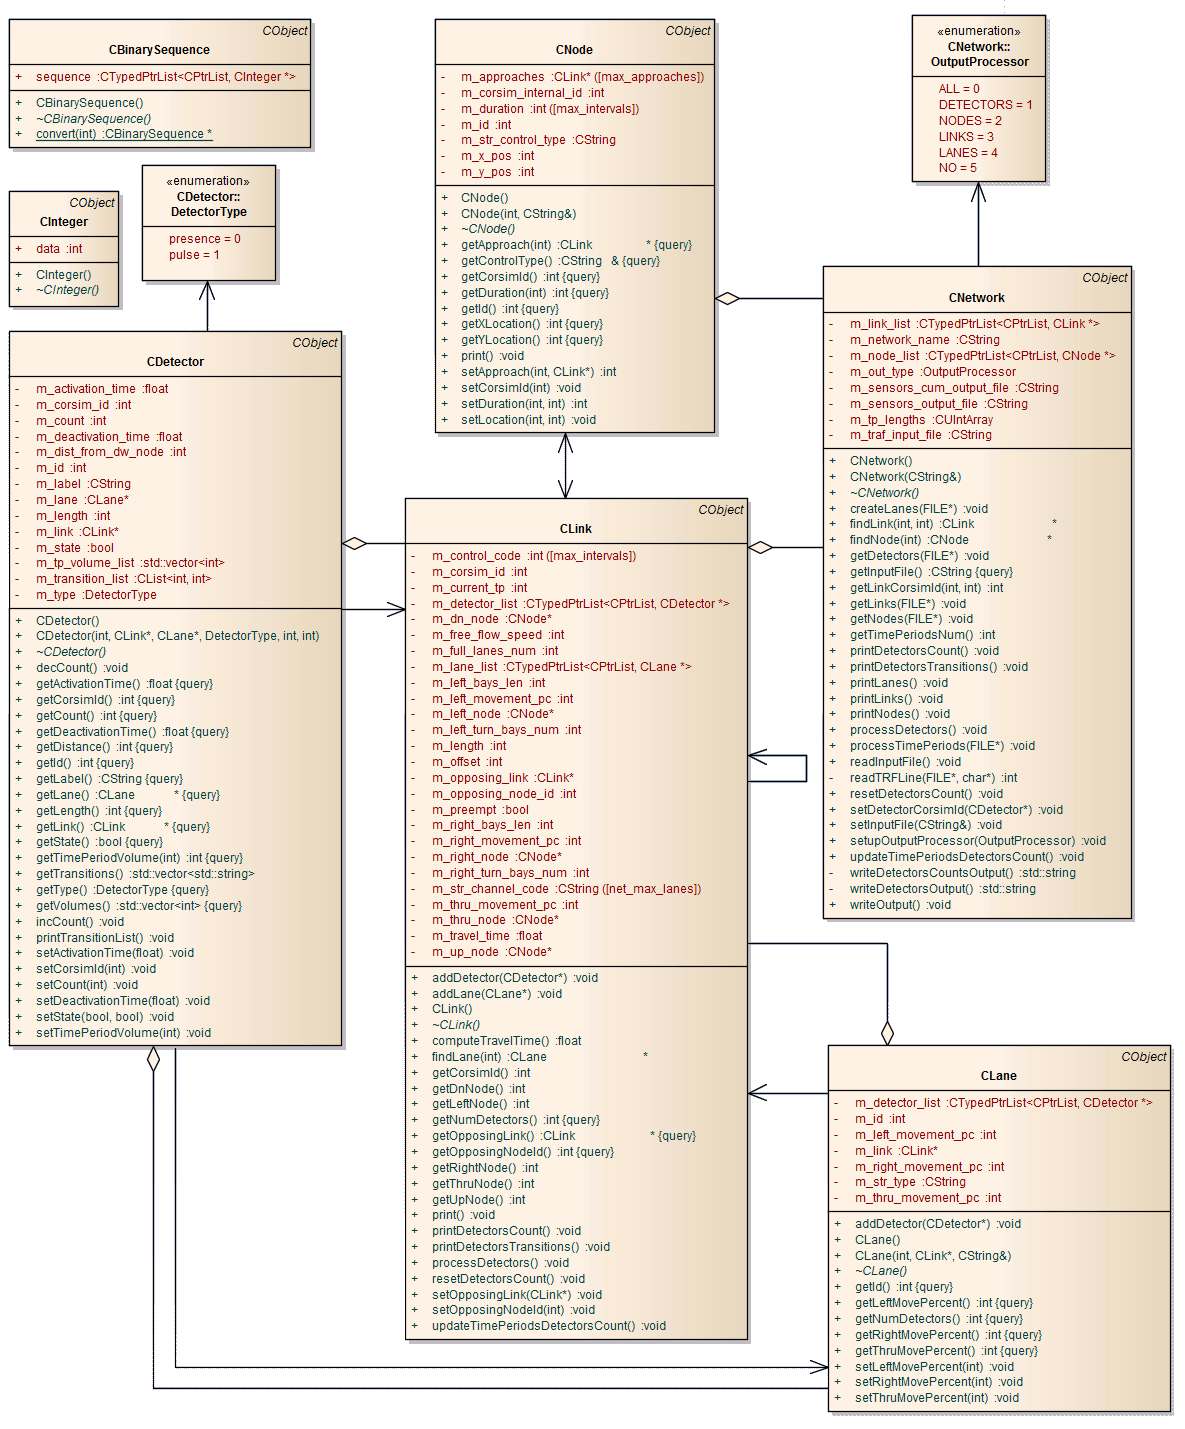
\includegraphics[width=1.4\textwidth,center]{sensors-class-diagram}
    \caption[Diagramma delle classi di \acsfont{Sensors} \acs{DLL}]{Diagramma delle classi di \acsfont{Sensors} \acs{DLL}.}
    \label{fig:sensors-class-diagram}
\end{figure}

\subsection{Formato dell'output}\label{subsec:sensors-dll-output}
Di seguito si presenta un esempio di file \acs{CSV} di output generato da \acsfont{Sensors} \acs{DLL}. Come anticipato, esso codifica l'\keyword{onda quadra} di ogni sensore a spira magnetica posto sulla rete stradale.

\vspace*{8pt}\inputsourcecode[language=pseudo, numbers=none, caption=Formato di output di \acsfont{Sensors} \acs{DLL}, label=lst:sensors-out-format]{codes/sensorsoutformat.txt}

La~\vref{tab:sensors-output-semantic} chiarisce il significato di ogni colonna dei dati tabulari restituiti da \acsfont{Sensors} \acs{DLL}.
\begin{table}[H]%
\begin{tabularx}{\columnwidth}{+l^X}
\toprule\rowstyle{\bfseries}%
Nome colonna            & Descrizione                                                                       \\
\otoprule%
time                    & Tempo di simulazione a cui è stato effettuato il monitoraggio dei sensori.        \\
tp                      & Indice del corrente periodo temporale (\ie{} \emph{time period}).                \\
identificatore sensore  & $1$ in caso di presenza di un veicolo sul rispettivo sensore, $0$ altrimenti.    \\\bottomrule
\end{tabularx}
\caption[Semantica dell'output di \acsfont{Sensors} \acs{DLL}]{Descrizione della semantica dei file \acs{CSV} generati da \acsfont{Sensors} \acs{DLL}.}
\label{tab:sensors-output-semantic}
\end{table}

Si osservi che, il fatto che il sensore \lstinline[]|D232|, in corrispondenza dell'istante $1.6$ ($5$\textsuperscript{a} colonna) abbia valore $1$ non indica che il veicolo sia stato rilevato esattamente in tale istante, bensì ciò indica che durante l'intervallo temporale $[\,1.5,1.6\,]$ tale sensore è stato attivato dal passaggio di un veicolo.

\cleardoublepage
\section{Applicativi di supporto}\label{sec:dataset-tools}
Al fine di automatizzare e facilitare la creazione di dataset relativi al traffico tramite la \acs{RTE} trattata nel corrente capitolo, si è sviluppato un insieme di strumenti dediti alla manipolazione dei file di output di \acsfont{Sensors} \acs{DLL}.

Di seguito si elencano le operazioni di manipolazione che tali strumenti supportano:
\begin{enumerate}
    \item sostituzione (e eventualmente rimozione) della colonna relativa ai periodi temporali con una nuova colonna che rappresenti la classe di un insieme di osservazioni; tale colonna è automaticamente generata in base a un sistema di regole (\eg{} \emph{matching} tra periodo temporale e classe).
    \item partizionamento del file di output di \acsfont{Sensors} \acs{DLL} in più file in base a vincoli temporali (\eg{} divisione del file in blocchi di $60$ secondi ciascuno)
    \item ottimizzazione del file tramite rimozione delle linee duplicate (\ie{} linee in cui non è avvenuto alcun cambiamento di stato dei sensori).
\end{enumerate}

% !TEX encoding = UTF-8
% !TEX TS-program = pdflatex
% !TEX root = ../arsclassica.tex
% !TEX spellcheck = it-IT

%************************************************
\chapter{Esperimenti numerici}
\label{cap:esperimenti}
%************************************************

\lipsum[1]

\section{Dataset \texorpdfstring{$1$}{1}}
\lipsum[2]

\subsection{Modello TSIS}
\lipsum[3]

\subsection{Risultati}
\lipsum[4]

\section{Dataset \texorpdfstring{$2$}{2}}
\lipsum[5]

\subsection{Modello TSIS}
\lipsum[6]

\subsection{Risultati}
\lipsum[7]

% !TEX encoding = UTF-8
% !TEX TS-program = pdflatex
% !TEX root = ../arsclassica.tex
% !TEX spellcheck = it-IT

%************************************************
% Conclusioni
%************************************************
\cleardoublepage
\phantomsection
\markboth{\spacedlowsmallcaps{Conclusione}}{\spacedlowsmallcaps{Conclusione}}
\addcontentsline{toc}{chapter}{\tocEntry{Conclusioni}}
\chapter*{Conclusioni}\label{cap:concl}
Questo lavoro di tesi è stato incentrato sul framework delle \acf{CTBN}, e sulla descrizione di una classe di modelli di \emph{classificatori} da esso derivanti.

Come ampiamente descritto e motivato, il principale vantaggio apportato dalle \acs{CTBN} consiste nella loro capacità di rappresentare esplicitamente \emph{sistemi dinamici} che evolvono nel \emph{tempo continuo} senza necessitare della scelta a priori di un'arbitraria granularità temporale, a differenza di altri modelli grafico probabilistici con scopi simili (\eg{} \acl{DBN}). Inoltre, tale modello non possiede il vincolo di aciclicità. Ciò permette di modellare in modo naturale le mutue influenze fra le variabili di un dato sistema dinamico, e di facilitare il processo di apprendimento strutturale, permettendo di ricercare l'insieme di nodi genitori di ogni nodo in modo indipendente da quello dei restanti nodi del modello.

Si è quindi descritto il processo di \emph{apprendimento dei parametri} per le \acs{CTBN} e il conseguente algoritmo di \emph{apprendimento dei classificatori} \acs{CTBN} (\acs{CTBNC}), entrambi relativi a dati completi. Come naturale prosecuzione del processo di apprendimento dei classificatori si è descritto l'algoritmo di \emph{inferenza esatta} per i \acs{CTBNC}, il quale implementa un \emph{tradeoff} fra complessità computazionale e efficacia di classificazione.

Come detto, i classificatori \acs{CTBN} (\acs{CTBNC}) sono un modello grafico probabilistico applicabile al problema della \emph{classificazione supervisionata} nel caso in cui le seguenti condizioni sussistano:
\begin{itemize}
	\item gli attributi sono discreti (o discretizzabili)
	\item il tempo fluisce continuamente
	\item si dispone di dati completi
	\item la classe si verifica nel futuro.
\end{itemize}

Si è infine descritto un processo di \emph{apprendimento strutturale} basato sull'ottimizzazione, attuata tramite una procedura di ricerca euristica (\ie{} \emph{\hc{}}), di una \emph{funzione di punteggio} per le \acs{CTBN}.

Nella seconda parte del presente elaborato, invece, si sono affrontati argomenti di tipo pratico.

In primis, si è presentato \rctbn{}, il \emph{pacchetto} \lstinline$R$ sviluppato al fine di implementare il framework delle \acs{CTBN} e gli algoritmi descritti nella parte teorica della tesi.

Successivamente si è descritto il software commerciale \acs{TSIS} utilizzato per la \emph{modellazione di profili di traffico su reti stradali urbane} e \acsfont{Sensors} \acs{DLL}, una sua \acl{RTE} sviluppata al fine di monitorare e tracciare il passaggio dei veicoli sui \emph{sensori} presenti in tali reti stradali.

La progettazione e l'implementazione di tali applicativi si è resa necessaria allo scopo di generare dei \emph{dataset} che rappresentassero dei sistemi dinamici complessi, qual è il traffico automobilistico, da sottoporre ai classificatori \acs{CTBN} (\acs{CTNBC}). Grazie a tali dataset si è potuto effettuare una \emph{sperimentazione} di $4$ diverse istanze di classificatori \acs{CTBN} allo scopo di valutare la loro applicazione a un problema noto e complesso qual è la \emph{classificazione dei profili di traffico}.

Tale sperimentazione ha permesso inoltre di comparare l'efficacia dei vari modelli di classificatore \acs{CTBN} utilizzati: il classificatore \acl{CTNB} (\acs{CTNBC}) e i classificatori appresi tramite il succitato algoritmo di apprendimento strutturale. Dai \emph{risultati} ottenuti si è evinto che tali modelli ottengono un buon livello di classificazione. Tuttavia, a causa della natura dei sistemi dinamici descritti dei dataset, non si sono rilevate differenze notabili fra i vari modelli di classificatori utilizzati.

Ciò pone quindi un primo spunto per gli eventuali \emph{sviluppi futuri} del corrente lavoro di tesi: l'elaborazione di una procedura di apprendimento strutturale alternativa che porti all'ottenimento di classificatori \acs{CTBN} maggiormente efficaci.

Riguardo tale argomento, è sicuramente di notevole interesse, per i risvolti che ciò può comportare, affrontare nel futuro gli stessi argomenti presentati in questo lavoro di tesi relativamente però a insiemi di dati non completamente osservati.

Anche dal punto di vista pratico, questo lavoro di tesi può essere esteso in vari modi. Ad esempio, l'applicativo per la generazione di dataset relativi al traffico necessita di conformare completamente i dati che esso genera alla forma che le \acs{CTBN} richiedono. Ci si riferisce, nello specifico, alla rilevazione degli istanti temporali in cui più di un sensore effettua una transizione di stato. \`E importante rimarcare, infatti, che i modelli \acs{CTBN} assumono che due variabili non possano effettuare una transizione contemporaneamente. Tale assunzione può essere vista come una formalizzazione del fatto che le variabili devono rappresentare aspetti distinti del mondo: in generale, non si dovrebbe modellare un dominio in cui due o più variabili cambiano stato contemporaneamente in modo deterministico.

% *****************************************************************
% Backmatter
%******************************************************************
\appendix
% !TEX encoding = UTF-8
% !TEX TS-program = pdflatex
% !TEX root = ../arsclassica.tex
% !TEX spellcheck = it-IT

%************************************************
\chapter{Guide all'uso}
\label{cap:guide}
%************************************************
Lo scopo di questa appendice è formulare delle guide all'utilizzo del software sviluppato a sostengo del lavoro di tesi.

Questa appendice è quindi suddivisa in due sezioni tematiche, una relativa all'utilizzo delle principali funzionalità offerte dal \pacchettor{} e una relativa all'utilizzo di \acsfont{Sensors} \acs{DLL} per la generazione di dataset da modelli \acs{TSIS}.

Tutti gli esempi presentati in questa appendice si riferiscono alla variante estesa, con elementi da $100$ secondi, del dataset relativo a \emph{Viale Cesare Battisti} (\ie{} \ds{2\text{.}E\text{.}100}). In questo capitolo, per brevità, ci si riferirà a tale dataset semplicemente con il termine \ds{2}.

\section{Utilizzo del pacchetto RCTBN}\label{sec:package-howto}
Nelle seguenti sottosezioni si illustrano le funzionalità principali offerte da \rctbn{}. Lo scopo è quello di guidare l'utente all'utilizzo del framework delle \acs{CTBN} tramite il succitato pacchetto \lstinline[]|R|.

Prima di addentrarci nella guida all'utilizzo del \pacchettor{} è necessario verificare che il sistema disponga dell'adeguato ambiente \lstinline[]|R| (versione $\ge 3.0$). Inoltre è necessario che il pacchetto \lstinline[]|devtools|\footnote{Il pacchetto \lstinline[]|devtools| è un insieme di funzioni e strumenti finalizzati all'espletamento di processi comuni e fondamentali per lo sviluppo in \lstinline[]|R|. Il codice sorgente di tale pacchetto è disponibile all'indirizzo: \url{https://github.com/hadley/devtools}.} sia correttamente installato. In caso contrario, purché si disponga di una connessione a Internet, è possibile installare l'ultima versione stabile digitando il seguente comando in una nuova sessione \lstinline[]|R|.

\vspace*{8pt}\inputsourcecode[caption={[Installazione del pacchetto \lstinline$devtools$]Installazione del pacchetto \lstinline$devtools$.},language=rstats,numbers=none]{codes/devtoolsinstallation}

A questo punto è possibile procedere all'installazione del \pacchettor{}. Poiché esso non è ancora stato pubblicato nell'archivio online dei pacchetti \lstinline$R$\footnote{Una delle modalità di installazione di pacchetti \lstinline$R$ è tramite connessione a un archivio online in cui essi vengono memorizzati. Tale archivio, chiamato \acf{CRAN}, è raggiungibile al seguente indirizzo: \url{http://cran.r-project.org}.}, la procedura di installazione differisce da quella precedentemente mostrata. A tale scopo si utilizza quindi il pacchetto \lstinline$devtools$ per installare \rctbn{}. Si osservi che il pacchetto \lstinline$devtools$ permette di creare e installare un pacchetto \lstinline$R$ a partire dal suo sorgente (purché esso rispetti le dovute convenzioni e contenga codice eseguibile senza errori), che sia esso online o sul sistema dell'utente, o da un archivio compresso. Perciò, disponendo del sorgente di \rctbn{}, è possibile installarlo come pacchetto \lstinline$R$ digitando le seguenti istruzioni.

\vspace*{8pt}\inputsourcecode[caption={[Installazione del \pacchettor{}]Installazione del \pacchettor{}.},language=rstats]{codes/rctbninstallation}

Si osservi che l'opzione \lstinline$dependencies$ fa sì che tutte i pacchetti da cui \rctbn{} dipende vengano scaricati e installati dall'archivio \acs{CRAN}: anche in questo caso è quindi necessaria una connessione a Internet.

\`E ora possibile utilizzare il \pacchettor{} per l'esecuzione dei vari processi relativi al framework delle \acs{CTBN}. Si osservi che esso viene installato con il nome \lstinline$ctbn$ nella libreria \lstinline$R$.

Tutti gli esempi d'utilizzo che vengono mostrati in questa sezione assumono che la cartella di lavoro sia \lstinline[language=rstats]{"~/Workspace/R/test/ctbn"}. Perciò, come mostrato in seguito, si utilizza il comando \lstinline$setwd$ per impostare la cartella di lavoro.

\subsection{Gestione dei dataset}
Come detto nella \autoref{subsec:rctbn-ds-management} \vpageref{subsec:rctbn-ds-management}, il \pacchettor{} implementa una serie di funzionalità, non correlate concettualmente al framework delle \acs{CTBN}, utili allo svolgimento di operazioni di gestione dei dataset. Lo scopo principale di questo insieme di funzionalità è permettere il caricamento e la compressione su disco dei dataset per le \acs{CTBN}, così da evitare all'utente la ripetizione di tale operazione ogni qual volta egli necessiti di un dataset precedentemente già importato.

Perciò, di seguito si illustra come importare il \ds{2} (descritto nella \vref{sec:dataset-2}).

\vspace*{8pt}\inputsourcecode[caption={[Importazione e serializzazione del \ds{2}]Importazione e serializzazione del \ds{2}.},language=rstats,label=lst:rctbn-import-ds]{codes/importctbnds}
Si osservi che, come anticipato, è indispensabile impostare la corrente cartella di lavoro (comando \lstinline$setwd$) poiché il \pacchettor{} utilizza tale informazione per cercare il dataset da importare. Nello specifico, \rctbn{} cercherà nella cartella di lavoro una cartella \lstinline$dataset$ e dentro questa cercherà una cartella con il nome del primo parametro attuale della funzione \lstinline[language=rstats]{read_dataset}. \`E possibile modificare la cartella in cui \rctbn{} cerca i dataset modificando l'opzione \lstinline$ctbn.data.dir$, impostata di default al valore \lstinline$dataset$, tramite il comando \lstinline[language=rstats]{options}.

La funzione \lstinline[language=rstats]{read_dataset} effettua varie operazioni, che vengono descritte di seguito.
\begin{itemize}
	\item Legge ogni file \acs{CSV} presente nella cartella:\par
	\lstinline[language=rstats]{"~/Workspace/R/test/ctbn/dataset/monza100e"}.\par
	\`E possibile importare file con altre estensioni semplicemente modificando il valore dell'opzione \lstinline$ctbn.data.ext$, impostato all'avvio al valore \lstinline[language=rstats]{"csv"}.
	\item Controlla che ogni struttura tabulare letta contenga la colonna relativa al tempo. Tale informazione è specificabile tramite l'opzione \lstinline$ctbn.col.time$, impostata di default al valore \lstinline[language=rstats]{"time"}.
	\item Controlla che ogni struttura tabulare letta contenga la colonna relativa alla classe. Tale informazione è specificabile tramite l'opzione \lstinline$ctbn.col.class$, impostata all'avvio a \lstinline[language=rstats]{"class"}. Nel caso in cui non si sia interessati ad eseguire tale controllo è possibile ometterlo semplicemente modificando la chiamata in questione come mostrato di seguito:\par
	\lstinline[language=rstats]{read_dataset("monza100e", classcheck = FALSE)}.
	\item Controlla che ogni file contenga altre colonne oltre a quelle relative al tempo e, opzionalmente, alla classe.
	\item Ordina le strutture tabulari importati in base alle rispettive colonne temporali.
	\item Crea un oggetto \lstinline$R$ simile a una tabella hash dove ogni chiave è rappresentata da una stringa, il nome del file importato (senza estensione), e ogni elemento è una tabella (nello specifico un oggetto della classe \lstinline$data.table$) contenente la struttura tabulare importata.
	\item Serializza in modo compresso tale oggetto su file salvando un file \acsfont{RDATA}\footnote{I file con estensione \acsfont{RDATA}, o \acsfont{RDA}, sono dei formati binari che \lstinline$R$ utilizza per la memorizzazione su disco di oggetti appartenenti al suo linguaggio.} nella cartella adibita alla memorizzazione dei dataset importati (specificata dall'opzione \lstinline$ctbn.store.dir$, il cui valore di default è \lstinline[language=rstats]{"data"}). \`E possibile, ma non consigliato, disattivare la serializzazione del dataset importato modificando la chiamata in questione come mostrato:\par
	\lstinline[language=rstats]{read_dataset("monza100e", autosave = FALSE)}.
\end{itemize}

L'output del sorgente \ref{lst:rctbn-import-ds} corrisponde all'oggetto \lstinline$R$ contenente il dataset nelle modalità descritte. Ciò significa che assegnando tale funzione a una variabile sarà possibile operare con il dataset in questione. Ad esempio:

\lstinline[language=rstats]{monzads = read_dataset("monza100e")}.

Si osservi che, nel caso in cui non l'opzione \lstinline$ctbn.verbose$ (posta di default a \lstinline[language=rstats]{TRUE}) non sia stata modificata, la funzione \lstinline[language=rstats]{read_dataset} stampa a video il seguente messaggio:

\vspace*{8pt}\inputsourcecode[language=rstats,nolol,numbers=none,basicstyle=\footnotesize\ttfamily]{codes/importctbndsoutput}\vspace*{8pt}

Quindi, eseguito il sorgente \ref{lst:rctbn-import-ds}, il dataset sarà stato importato e serializzato come oggetto \lstinline$R$ al seguente percorso:

\lstinline[language=rstats]{"~/Workspace/R/test/ctbn/data/monza100e/store.rdata"}.

Si osservi che anche tale comportamento è personalizzabile tramite l'utilizzo delle opzioni che \rctbn{} fornisce all'utente. Nello specifico è possibile modificare l'opzione \lstinline$ctbn.store.name$, impostata di default al valore \lstinline[language=rstats]{"store"}, e l'opzione \lstinline$ctbn.store.ext$, impostata all'avvio al valore \lstinline[language=rstats]{"rdata"}.

Si mostra ora come sfruttare l'operazione appena illustrata per utilizzare il \ds{2} in una nuova sessione \lstinline$R$ senza necessità di importarlo nuovamente, processo che ha richiesto circa $45$ secondi. Tale caratteristica di \rctbn{} permette di ottenere un notevole risparmio di tempo nel flusso di lavoro.

\vspace*{8pt}\inputsourcecode[caption={[Caricamento del \ds{2}]Caricamento del \ds{2}.},language=rstats,label=lst:rctbn-load-ds]{codes/loadctbnds}
Come detto, la funzione \lstinline[language=rstats]{load_dataset} non importa nuovamente il dataset \lstinline[language=rstats]{"monza100e"}, bensì essa cerca il relativo file \acsfont{RDATA} nella cartella apposita e inietta dinamicamente l'oggetto da esso contenuto nell'attuale ambiente \lstinline$R$. Ciò significa che l'esecuzione del sorgente \ref{lst:rctbn-load-ds} permette di avere istantaneamente accesso a una oggetto \lstinline$R$ memorizzato in una variabile \lstinline$monza100e$.

Si osservi infine che l'intero processo di gestione dei dataset contempla la possibilità che l'utente utilizzi dei dataset il cui nome non corrisponde a un nome di variabile valido per \lstinline$R$. In tale situazione il \pacchettor{} provvede a generare un nome di variabile valido a partire dal nome del dataset specificato. Perciò, una volta importato o caricato tale dataset sarà possibile ricavare il suo nome ispezionando l'ambiente \lstinline$R$ eseguendo il comando \lstinline[language=rstats]{ls(all = TRUE)}, il quale elenca tutte le variabili disponibili nell'ambiente \lstinline$R$ attuale. Alternativamente, qualora l'opzione \lstinline$ctbn.verbose$ abbia valore \lstinline[language=rstats]{TRUE}, la funzione \lstinline[language=rstats]{load_dataset} mostrerà a video un messaggio, finalizzato alla comunicazione del nome della variabile in cui il dataset è stato iniettato.

\vspace*{8pt}\inputsourcecode[language=pseudo,nolol,numbers=none,basicstyle=\footnotesize\ttfamily]{codes/loadctbndsoutput}

\subsection{Calcolo delle \stats{}}
In questa sottosezione si illustrano le funzionalità che \rctbn{} fornisce affinché l'utente possa computare le \emph{\stats{}}.

I sorgenti mostrati assumono che il \pacchettor{} sia stato caricato e che il \ds{2} sia stato importato e caricato.

Si suppone innanzitutto di voler calcolare le \emph{\stats{}} di una o più variabili del \ds{2} dato uno specifico insieme di genitori. A tale scopo \rctbn{} fornisce la funzione \lstinline[language=rstats]{fsstats}.

Perciò, di seguito si illustra come computare le \emph{\stats{}} su tutto il \ds{2} del nodo \lstinline[language=rstats]{"D241"} impostando come suo insieme dei genitori l'insieme composto dai nodi \lstinline[language=rstats]{"D911"}, \lstinline[language=rstats]{"D191"} e \lstinline[language=rstats]{"D641"}.

\vspace*{8pt}\inputsourcecode[caption={[Calcolo delle \stats{} sul \ds{2}]Esempio di calcolo delle \emph{\stats{}} sul \ds{2}.},language=rstats,label=lst:rctbn-fsstats]{codes/fsstats}
Il risultato di tale esecuzione è una tabella hash contenente un solo elemento: le \emph{\stats{}} del nodo \lstinline[language=rstats]{"D241"} dati i nodi genitori \lstinline[language=rstats]{"D911"}, \lstinline[language=rstats]{"D191"} e \lstinline[language=rstats]{"D641"}. La chiave di tale elemento della tabella hash è una rappresentazione di tale informazione mentre l'elemento è un oggetto tabulare (classe \lstinline$data.table$) rappresentante i valori delle \emph{\stats{}} $T$ e $M$ per ogni combinazione dei valori assunti dai nodi genitori.

Di seguito si riporta l'output fornito dal sorgente \ref{lst:rctbn-fsstats}.

\vspace*{8pt}\inputsourcecode[language=pseudo,nolol,numbers=none,basicstyle=\footnotesize\ttfamily]{codes/fsstatsres}\vspace*{8pt}

Si osservi che \lstinline[language=rstats]{fsstats} non permette di computare le \emph{\stats{}} di più variabili specificando per ognuna di esse un insieme di genitori diverso. Tale funzione è quindi utilizzabile con profitto nel caso in cui si intenda calcolare le \emph{\stats{}} di più variabili (eventualmente anche tutte) rispetto a un unico insieme di genitori: si pensi ad esempio a ciò che è necessario fare quando si intende apprendere un classificatore \acs{CTNB} (\acs{CTNBC}) (mostrato in \vref{fig:ctnbc}), caratterizzato proprio dal fatto che ogni sua variabile ha un solo nodo genitore, il nodo classe.

Ipotizziamo perciò di volere utilizzare la funzione \lstinline[language=rstats]{fsstats} per calcolare le \emph{\stats{}} di alcune variabili (ad esempio le variabili \lstinline[language=rstats]{"D241"}, \lstinline[language=rstats]{"D781"} e \lstinline[language=rstats]{"D782"}) data la sola variabile \lstinline[language=rstats]{"class"} (\ie{} nodo classe) come genitore. Il sorgente che segue illustra come espletare tale obiettivo.

\vspace*{8pt}\inputsourcecode[language=rstats,caption={[Calcolo delle \stats{} sul \ds{2}]Esempio di calcolo delle \emph{\stats{}} di più nodi dato un insieme di genitori comune, il nodo classe (\ds{2}).},label=lst:rctbn-fsstats2]{codes/fsstats2}

Come visibile dall'output conseguente l'esecuzione del sorgente \ref{lst:rctbn-fsstats2}, in questo caso, la funzione \lstinline[language=rstats]{fsstats} restituisce una tabella hash con più elementi, una per ogni nodo oggetto della computazione delle \emph{\stats{}}.

\vspace*{8pt}\inputsourcecode[nolol,language=pseudo,numbers=none, basicstyle=\footnotesize\ttfamily]{codes/fsstats2res}\vspace*{8pt}

Si osservi che la funzione \lstinline[language=rstats]{fsstats} permette anche di calcolare le \emph{\stats{}} di uno o più nodi senza condizionare la loro computazione ad alcun genitore.

Di seguito viene illustrato come effettuare tale operazione.

\vspace*{8pt}\inputsourcecode[language=rstats,caption={[Calcolo delle \stats{} sul \ds{2}]Esempio di calcolo delle \emph{\stats{}} di un nodo senza condizionare la computazione a un insieme di genitori (\ds{2}).},label=lst:rctbn-fsstats3]{codes/fsstats3}

Nel caso in cui si desideri computare le \emph{\stats{}} di più nodi rispetto a diversi insiemi di genitori è invece necessario utilizzare la funzione \lstinline[language=rstats]{fsstats_graph}. La differenza tra tale funzione e quella appena illustrata consiste principalmente nella firma. Infatti, essa non richiede in input un parametro relativo ai nodi e uno relativo all'insieme di genitori comune, bensì una matrice binaria avente sulle righe i nodi genitori e sulle colonne i nodi figli, il cui scopo è rappresentare la struttura di una \acs{CTBN}. Un $1$ posto nella posizione $(3,2)$ (\ie{} riga $3$, colonna $2$) indica che il nodo $2$ è figlio del nodo $3$.

A titolo esemplificativo si ipotizzi di voler calcolare le \emph{\stats{}}:
\begin{itemize}
	\item del nodo \lstinline[language=rstats]{"D241"} dato il solo nodo \lstinline[language=rstats]{"class"} come genitore
	\item del nodo \lstinline[language=rstats]{"D781"} dati nodi genitori \lstinline[language=rstats]{"D981"} e \lstinline[language=rstats]{"D241"}
	\item del nodo \lstinline[language=rstats]{"D782"} dati nodi genitori \lstinline[language=rstats]{"class"} e \lstinline[language=rstats]{"D981"}.
\end{itemize}
Tale insieme di informazioni corrisponde alla matrice mostrata dalla seguente tabella.
\begin{table}[ht]
	\centering\footnotesize
	\begin{tabular}{+l^c^c^c}
	\toprule\rowstyle{\bfseries}%
	       			& D241   & D781 & D782 		\\\otoprule
	\bfseries{class}& $1$    & $0$ 	& $1$ 		\\
	\bfseries{D981} & $0$    & $1$ 	& $1$ 		\\
	\bfseries{D241} & $0$    & $1$ 	& $0$ 		\\\bottomrule
	\end{tabular}
	\caption[Struttura d'esempio di una \acs{CTBN}]{Struttura d'esempio di una \acs{CTBN} espressa tramite la corrispondenza fra i nodi e relativi insiemi di genitori.}
	\label{tab:little-example-ctbn}
\end{table}

Il sorgente che segue illustra come costruire tale matrice e utilizzarla come parametro di input della funzione \lstinline[language=rstats]{fsstats_graph}.

\vspace*{8pt}\inputsourcecode[language=rstats,caption={[Calcolo delle \stats{} sul \ds{2}]Esempio di calcolo delle \emph{\stats{}} di più nodi aventi diversi insiemi di nodi genitori (\ds{2}).},label=lst:rctbn-ffstatsgraph]{codes/fsstatsgraph}

L'output ottenuto dall'esecuzione del sorgente \ref{lst:rctbn-ffstatsgraph} illustra le \emph{\stats{}} dei nodi scelti, dati i loro rispettivi insiemi di nodi genitori, computate sul \ds{2}.

\vspace*{8pt}\inputsourcecode[numbers=none,language=pseudo,nolol,basicstyle=\footnotesize\ttfamily]{codes/fsstatsgraphres}

\subsection{Apprendimento dei parametri}
Si illustra ora come effettuare l'apprendimento dei parametri di una \acs{CTBN} da un insieme di \emph{\keyword{dati completi}}, nello specifico dal \ds{2}, tramite la relativa funzionalità offerta dal \pacchettor{}. Si ricorda, come discusso nella \autoref{subsec:ctbn-params} \vpageref{subsec:ctbn-params}, che è possibile effettuare la \keyword{stima dei parametri} tramite due approcci: la \keyword{stima \acl{MLE}} o la \keyword{stima bayesiana}.

Supponendo di considerare la \acs{CTBN} con la struttura utilizzata per l'esempio precedente (si veda la \vref{tab:little-example-ctbn}) e di aver salvato le \emph{\stats{}} calcolate nel sorgente \ref{lst:rctbn-fsstats2} in una variabile chiamata \lstinline$ss$, è possibile apprendere i parametri fornendo tale variabile in input alla funzione \lstinline[language=rstats]{params}.

\inputsourcecode[caption={[Stima dei parametri di una \acs{CTBN} dal \ds{2}]Apprendimento (\ie{} stima esatta) dei parametri di una \acs{CTBN} dal \ds{2}.},language=rstats,label=lst:rctbn-hparams]{codes/params}

Tale funzione richiede in input una tabella hash contenente le \emph{\stats{}} di uno o più nodi (qualsiasi sia il loro insieme di genitori), cioè un oggetto restituito dalle funzioni \lstinline[language=rstats]{fsstats_graph} o \lstinline[language=rstats]{fsstats}.

L'output restituito è il seguente, dove le colonne \lstinline$T_PARAM$ e \lstinline$Q_PARAM$ si riferiscono rispettivamente ai parametri $\param{$\theta$}$ e $\param{q}$.

\vspace*{8pt}\inputsourcecode[language=pseudo,nolol,basicstyle=\footnotesize\ttfamily,numbers=none]{codes/paramsres}\vspace*{8pt}

Per controllare il modo in cui i parametri vengono computati, cioè se essi vengono appresi tramite stima \acl{MLE} o tramite \keyword{stima bayesiana}, il \pacchettor{} fornisce $3$ opzioni, presentate di seguito.
\begin{itemize}
	\item L'opzione \lstinline$ctbn.smoothing$, impostata al valore \lstinline[language=rstats]{TRUE} all'avvio di \rctbn{}. Ciò indica che, qualora non si modifichi tale opzione, \rctbn{} effettua la \emph{\keyword{regolarizzazione bayesiana}} dei parametri (corrispondente all'implementazione dell'\autoref{eq:ctbn-imaginary-params} \vpageref{eq:ctbn-imaginary-params})
	\item Le opzioni \lstinline$ctbn.imaginary.count$  e \lstinline$ctbn.imaginary.time$ utili a specificare i valori dei \emph{\keyword{conteggi immaginari}}. Esse sono impostate di dafault rispettivamente ai valori $1$ e $0.005$.
\end{itemize}
Perciò, l'esempio presentato dal sorgente \ref{lst:rctbn-hparams} effettua la \emph{\keyword{stima bayesiana}} dei parametri, calcolando $\paramhat{q}$ e $\greekhat{\theta}$.

\subsection{Calcolo delle CIM}
Riguardo il calcolo delle \im{} \cond{} (\acs{CIM}), il \pacchettor{} offre una funzione, \lstinline[language=rstats]{cims}, che è il naturale proseguimento della funzione \lstinline[language=rstats]{params} illustrata nella sottosezione precedente.

Per calcolare le \im{} \cond{} è necessario disporre di un oggetto, che chiamiamo \lstinline$pp$, contenente i parametri appresi tramite la funzione \lstinline[language=rstats]{params}. A tal fine è sufficiente modificare l'ultima linea del sorgente \ref{lst:rctbn-hparams} affinché il risultato della funzione \lstinline[language=rstats]{params} venga salvato in una variabile con tale nome.

La porzione di codice seguente illustra la chiamata di tale funzione.

\vspace*{8pt}\inputsourcecode[caption={[Calcolo delle \acs{CIM} di una \acs{CTBN} dal \ds{2}]Calcolo delle \acs{CIM} della \acs{CTBN} d'esempio dal \ds{2}.},language=rstats,label=lst:rctbn-cim-comput]{codes/cims}

Di seguito viene mostrato un estratto dell'output ottenuto dall'esecuzione del sorgente \ref{lst:rctbn-cim-comput}.

\vspace*{8pt}\inputsourcecode[language=pseudo,nolol,basicstyle=\footnotesize\ttfamily,numbers=none]{codes/cimsres}\vspace*{8pt}

\subsection{Apprendimento di un CTBNC}
In questa sottosezione si presenta l'utilizzo del \pacchettor{} per l'apprendimento di un classificatore \acs{CTBN} (\acs{CTBNC}).

A tale scopo si presenta una porzione di codice \lstinline$R$ che, generato in modo casuale un classificatore \acs{CTBN} valido (si veda la \autoref{defn:ctbnc} nella \vref{sec:ctbnc-model}) per il \ds{2}, utilizza la funzione \lstinline[language=rstats]{learn_ctbnc} per apprenderne i parametri e la distribuzione a priori delle classi rispetto a un \emph{\keyword{training set}} di tale dataset.

Prima di illustrare il sorgente necessario all'apprendimento del succitato classificatore \acs{CTBN}, si riporta la sua struttura tramite la \vref{tab:ex-ctbnc-tab}, la quale illustra l`insieme di nodi genitori di ogni nodo.

\begin{table}[H]%
	\footnotesize
	\centering%
	\begin{tabular}{+c^c}
	\toprule\rowstyle{\bfseries}%
	Nodo    			& Nodi genitori 											\\\otoprule
	D$1091$     	    & class, D$912$     										\\
	D$1092$     	    & class, D$1091$     										\\
	D$1110$     	    & class, D$5098$     										\\
	D$1290$     	    & class, D$5095$     										\\
	D$1480$     	    & class, D$212$, D$1110$ 									\\
	D$1681$     	    & class, D$982$     										\\
	D$1682$     	    & class, D$5094$,D$191$     								\\
	D$1687$     	    & class, D$541$, D$1290$, D$1092$     						\\
	D$191$     	    	& class     												\\
	D$192$     	  		& class     												\\
	D$211$     	    	& class, D$982$, D$1091$     								\\
	D$212$     	    	& class, D$5099$     										\\
	D$241$     	    	& class,     												\\
	D$242$     	    	& class, D$5096$, D$911$     								\\
	D$341$     	   		& class, D$242$, D$892$, D$1091$     						\\
	D$421$     	    	& class, D$241$, D$982$, D$1091$     						\\\bottomrule
	\end{tabular}
	\hspace{-0.6em}
	\begin{tabular}{+c^c}
	\toprule\rowstyle{\bfseries}%
	Nodo    			& Nodi genitori 											\\\otoprule
	D$5094$     	    & class, D$1092$, D$781$     								\\
	D$5095$     	    & class, D$5097$, D$982$, D$1091$     						\\
	D$5096$     	    & class, D$212$, D$1687$     								\\
	D$5097$     	    & class     												\\
	D$5098$     	    & class, D$341$   											\\
	D$5099$     	    & class   													\\
	D$541$     	    	& class, D$421$     										\\
	D$641$     	    	& class, D$341$, D$911$, D$192$     						\\
	D$781$     	    	& class 	     											\\
	D$782$     	 	    & class 	     											\\
	D$891$     	    	& class, D$242$     										\\
	D$892$     	 	    & class, D$241$, D$1682$, D$781$     						\\
	D$911$     	  	    & class     												\\
	D$912$     	  	    & class, D$5098$, D$892$    								\\
	D$981$     	        & class, D$341$, D$982$, D$1110$, D$781$     				\\
	D$982$				& class, D$5094$									 		\\\bottomrule
	\end{tabular}
	\caption[Struttura d'esempio di classificatore \acs{CTBN}]{Struttura d'esempio di un classificatore \acs{CTBN} (\acs{CTBNC}) espressa tramite la corrispondenza fra i nodi e relativi insiemi di genitori.}\label{tab:ex-ctbnc-tab}
\end{table}
\normalsize
Si osservi che tale struttura è perfettamente riproducibile su qualsiasi macchina esegua il codice utile a generarla. Ciò è possibile grazie all'utilizzo del comando \lstinline[language=rstats]{set.seed} che fissa il seme del generatore dei numeri casuali di \lstinline$R$.

Si presenta ora sinteticamente la firma della la funzione \lstinline[language=rstats]{learn_ctbnc}. Essa richiede in input due parametri principali:
\begin{itemize}
	\item il \emph{\keyword{training set}}
	\item una matrice di adiacenza, della stessa entità di quella richiesta dalla funzione \lstinline[language=rstats]{fsstats_graph}, che rappresenti una struttura valida di un classificatore \acs{CTBN}.
\end{itemize}
Tuttavia, si noti che essa prevede ulteriori parametri formali che non vengono presentati poiché non ritenuti di primaria importanza.

In sostanza, la funzione \lstinline[language=rstats]{learn_ctbnc} implementa l'\autoref{lst:ctbnc-learning} presentato \vpageref{lst:ctbnc-learning}.

Di seguito si illustra il codice sorgente che, utilizzando tale funzione (si veda la \autoref{lst:learn-ctbnc-func-line}), apprende un \acs{CTBNC} da un \emph{\keyword{training set}} del \ds{2} (\ie{} da una porzione di elementi di tale dataset).
Si noti che prima d'eseguire tale operazione, da \autoref{lst:gen-valid-ctbnc-start} a \autoref{lst:gen-valid-ctbnc-end}, viene generata una struttura valida e casuale per un classificatore \acs{CTBN}; a \autoref{lst:gen-fake-ts} viene invece generato l'ipotetico \emph{\keyword{training set}}.

\vspace*{8pt}\inputsourcecode[caption={[Apprendimento di un \acs{CTBNC} sul \ds{2}]Apprendimento di un classificatore \acs{CTBN}, la cui struttura viene generata in modo casuale, su un \emph{\keyword{training set}} facente parte del \ds{2}.},language=rstats,label=lst:rctbn-learc-ctbnc]{codes/learnctbnc}

\cleardoublepage
Affinché l'output ottenuto dall'esecuzione del sorgente \ref{lst:rctbn-learc-ctbnc} sia leggibile, se ne riporta solamente la sua prima parte.

\vspace*{8pt}\inputsourcecode[nolol,language=pseudo,basicstyle=\footnotesize\ttfamily,numbers=none]{codes/learnctbncres}\vspace*{8pt}

Si osservi che l'oggetto restituito dalla funzione \lstinline[language=rstats]{learn_ctbnc} è una lista etichettata (\ie{} un tipo del linguaggio \lstinline$R$ simile a una tabella hash) composta da $2$ elementi, chiamati \lstinline$priors$ e \lstinline$params$.

Ipotizzando di assegnare il risultato di \lstinline[language=rstats]{learn_ctbnc} a un oggetto chiamato \lstinline$model$, è possibile accedere ai suoi elementi tramite l'operatore \lstinline$R$ per liste nominate \lstinline[]|$|%
. Ad esempio, il comando \lstinline[]|model$priors| permette di accedere alla distribuzione di probabilità a priori della variabile classe come visibile dall'output mostrato.

\subsection{Classificazione di un CTNBC}
Appreso un classificatore \acs{CTBN} su un \emph{\keyword{training set}} è chiaramente possibile, come discusso in questo lavoro di tesi, utilizzarlo per compiere la classificazione\index{classificazione supervisionata} di una qualsiasi istanza del \emph{\keyword{test set}}. A tale scopo si necessita di un algoritmo di classificazione che, dato in input il modello di un classificatore appreso e una istanza da classificare, inferisca la classe a cui è più probabile che tale istanza appartenga.

Lo scopo di questa sottosezione è illustrare il processo di classificazione\index{classificazione supervisionata} tramite un modello di classificatore \acs{CTNB} (\acs{CTNBC}).

In questo lavoro di tesi, \vpageref{lst:ctbnc-inference}, si è presentato un algoritmo di inferenza (\autoref{lst:ctbnc-inference}) dedito alla classificazione tramite classificatori \acl{CTBN} (\acs{CTBNC}), classe di modelli di \emph{\keyword{classificazione supervisionata}} cui appartengono i modelli di classificatori \acs{CTNB}. Il \pacchettor{} fornisce tale procedura di inferenza esponendo la funzione \lstinline[language=rstats]{infer_ctbnc}.

Prima di presentare la succitata funzione, si fa notare che \rctbn{} fornisce una funzione apposita per l'apprendimento dei classificatori \acs{CTNB} (\acs{CTNBC}): \lstinline[language=rstats]{learn_ctnbc}. Una chiamata a tale funzione è equivalente a una chiamata alla funzione \lstinline[language=rstats]{learn_ctbnc} con parametro \lstinline$amat$ posto al valore \lstinline$NULL$. Tuttavia, essa è ben più performante di \lstinline[language=rstats]{learn_ctbnc} poiché attua delle ottimizzazioni di calcolo dovute a delle assunzioni che la struttura dei classificatori \acs{CTNB} permettono di fare.

I parametri principali per cui la funzione \lstinline[language=rstats]{infer_ctbnc} richiede un input sono:
\begin{itemize}
	\item il modello di un classificatore \acs{CTBN} (\acs{CTBNC})
	\item un'istanza su cui effettuare la procedura di inferenza.
\end{itemize}
Anche in questo caso si tralascia la discussione dei restanti parametri poiché essi non sono di primaria importanza.

Di seguito si presenta il sorgente che, selezionata un'istanza dal \ds{2} (\ie{} il primo elemento nel dataset), apprende un classificatore \acs{CTNB} sui restanti elementi presenti del dataset (\autoref{lst:learn-ctbnc-infer1}) e utilizza tale modello per classificare la succitata istanza (\autoref{lst:infer-ctbnc-infer1}).

\cleardoublepage
\inputsourcecode[caption={Apprendimento di un classificatore \acs{CTNB} (\acs{CTNBC}) tramite la procedura generica e classificazione di un'istanza del \ds{2} tramite tale classificatore.},nolol,language=rstats]{codes/inferctnbc}

Come detto, utilizzando l'apposita funzione (si veda \autoref{lst:learn-ctbnc-infer2}) di apprendimento dei classificatori \acs{CTNB} (\acs{CTNBC}) è possibile ridurre la quantità di linee di codice e di operazioni necessarie, come mostra il seguente sorgente.

\vspace*{8pt}\inputsourcecode[caption={[Classificazione di un'istanza del \ds{2}]Apprendimento di un classificatore \acs{CTNB} (\acs{CTNBC}) tramie la apposita funzione e classificazione di un'istanza del \ds{2} tramite tale classificatore.},label=lst:rctbn-infer-ctnbc,language=rstats]{codes/inferctnbc2}

L'output della funzione \lstinline[language=rstats]{infer_ctbnc} consiste in una lista etichettata composta due elementi: \lstinline$logp$, contenente un vettore etichettato delle \emph{\keyword{log-probabilità}} di ogni classe e \lstinline$prob$, contenente un vettore etichettato delle \emph{\keyword{probabilità}} assegnate ad ogni classe del modello \acs{CTNBC} di riferimento.

\vspace*{8pt}\inputsourcecode[nolol,language=pseudo,numbers=none,basicstyle=\small\ttfamily]{codes/inferctnbcres}\vspace*{8pt}

Si osservi che, questa modalità di output non è l'unica che la funzione \lstinline[language=rstats]{infer_ctbnc} possiede. Infatti, fornendole un ulteriore parametro booleano in input, essa restituisce il nome (\ie{} classe $1$) della classe assegnata all'istanza processata e il relativo valore di probabilità ($100\%$, in questo caso). Nel caso si voglia operare manualmente tale operazione è sufficiente digitare il seguente comando:

\lstinline[language=rstats]{max(results[["prob"]])}.

\subsection{Apprendimento strutturale}
Lo scopo di questa sottosezione è presentare brevemente l'esecuzione del processo di \emph{\keyword{apprendimento strutturale}} tramite il \pacchettor{}.

Nello specifico, dato un ipotetico \emph{\keyword{training set}}, si presenta l'utilizzo della funzione \lstinline[language=rstats]{greedy_search} per l'apprendimento del classificatore \acs{CTBN} (\acs{CTBNC}) che meglio rappresenta tali \keyword{dati di addestramento}, fissato il numero massimo di genitori di ogni nodo al valore $2$. Tuttavia si osservi che la funzione in questione può apprendere una qualsiasi struttura \acs{CTBN}. Tale funzione esegue l'\autoref{lst:hc-pseudo}, presentato \vpageref{lst:hc-pseudo}, per ogni nodo delle istanze del \emph{\keyword{training set}}, utilizzando come punteggio la funzione $famscore_{\conceptsym{B}}$ presentata nella \vref{sec:ctbn-structurallearning-score} (si veda l'\autoref{eq:bayesian-score}).

La funzione \lstinline[language=rstats]{greedy_search} richiede che le siano fornite in input le seguenti informazioni, sotto forma di parametri:
\begin{itemize}
	\item un \emph{\keyword{training set}}
	\item \lstinline$method$, l'euristica da utilizzare per la \keyword{ricerca della struttura}
	\item \lstinline$fun$, la funzione di punteggio (\ie{} \emph{\keyword{score bayesiano}}) da utilizzare come criterio di selezione della struttura
	\item un punto di partenza, chiamato \lstinline$start$, da cui iniziare la ricerca, inteso come una matrice, eventualmente vuota, che rappresenti la struttura iniziale
	\item la lista \lstinline$excludelist$, eventualmente vuota, dei nodi da non sottoporre alla ricerca
	\item la lista \lstinline$whitelist$, eventualmente vuota, dei nodi che devono sempre far parte dell'insieme dei nodi genitori di ogni nodo su cui si effettua la ricerca
	\item la lista \lstinline$blacklist$, eventualmente vuota, dei nodi che non devono mai far parte dell'insieme dei nodi genitori di ogni nodo su cui si effettua la ricerca
	\item \lstinline$k$, la cardinalità massima degli insiemi dei nodi genitori.
\end{itemize}
Tuttavia, l'unico parametro obbligatorio è il \emph{\keyword{training set}}, sul quale la procedura di \keyword{ricerca euristica} computa lo \emph{\keyword{score bayesiano}} al variare dei nodi e del relativo insieme di genitori. I restanti parametri sono tutti dotati di un parametro di default.

Il sorgente che segue illustra come espletare il compito prefissatoci.

\vspace*{8pt}\inputsourcecode[caption={[Apprendimento della struttura]Apprendimento della struttura di un \acs{CTBN} (\acs{CTBNC}).},label=lst:rctbn-hc,language=rstats]{codes/hc}

L'output che tale funzione restituisce è composto dalla struttura che meglio rappresenta i \keyword{dati di addestramento} e il relativo modello \acs{CTBN} computato in fase di ricerca.

\section{Generazione di dataset}\label{sec:create-dataset-howto}
In questa sezione si illustra il processo di generazione di un dataset per le \acs{CTBN} a partire da un modello di traffico \acs{TSIS}, utilizzando l'\acl{RTE} sviluppata in questo lavoro di tesi, \acsfont{Sensors} \acs{DLL}.

\subsection{Sensors DLL}
Al fine di generare un dataset per le \acs{CTBN} che rappresenti l'\keyword{onda quadra} dei sensori a spira magnetica posti su una rete stradale \acs{TSIS} è necessario installare \acsfont{Sensors} \acs{DLL} in \acs{TShell}. Il processo di installazione, come già ampiamente specificato, consiste nel collegamento delle funzioni della succitata \acs{RTE} ai punti di chiamata predefiniti del modulo \acs{CORSIM}. L'intero processo di installazione, propedeutico alla generazione dei dataset, è stato illustrato nella \autoref{subsec:rte-corsim-linking} \vpageref{subsec:rte-corsim-linking}.

Si mostra il processo di generazione del \ds{2} (\vref{sec:dataset-2}).

Come primo passo è chiaramente necessario aprire \acs{TShell} e caricare il modello di traffico per i giorni lavorativi relativo a \emph{Viale Cesare Battisti}. Di seguito si elencano quindi i passi necessari alla generazione del \ds{2}:
\begin{itemize}
	\item nella barra degli strumenti di \acs{TShell} si clicchi l'icona relativa a \acsfont{Sensors} \acs{DLL}
	\item si clicchi sul pulsante relativo alle \emph{\virgolette{proprietà d'esecuzione}} $\vcenter{\hbox{
\includegraphics[scale=.9]{run-props}}}$ e successivamente sulla scheda \emph{\virgolette{proprietà d'esecuzione multipla}}
	\item si selezioni il file \acs{RNS} fornito in allegato a questo lavoro di tesi (e illustrato nel sorgente \ref{lst:model2-week-rns} \vpageref{lst:model2-week-rns}) come illustrato dalla \vref{fig:multi-run-properties-tsis-next}
	%\par
	%\begin{minipage}{\linewidth}
		%\centering
		%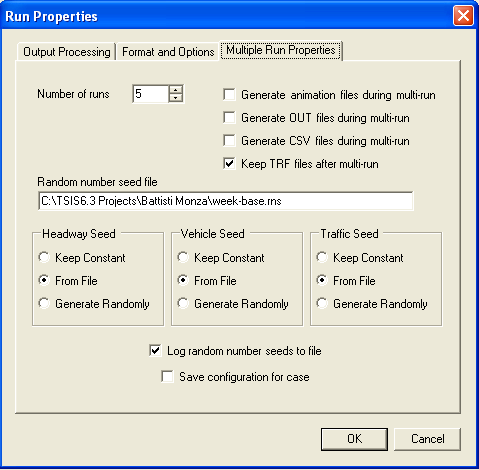
\includegraphics[width=.8\linewidth]{multi-run-properties-tsis-next}\captionof{figure}[Esecuzione multipla guidata da file \acs{RNS}]{Selezione del file \acs{RNS} per l'impostazione dell'esecuzione multipla.}\label{fig:multi-run-properties-tsis-next}
	%\end{minipage}
	\item si esegua la simulazione cliccando sull'apposito pulsante
	\item conclusa la simulazione, \acsfont{Sensors} \acs{DLL} salva, nella cartella dove il file \acs{TRF} simulato risiede, i file \acs{CSV} di output (riguardo il cui formato si è discusso nella \autoref{subsec:sensors-dll-output}~\vpageref{subsec:sensors-dll-output}).
\end{itemize}

\begin{figure}[ht]
	\centering
	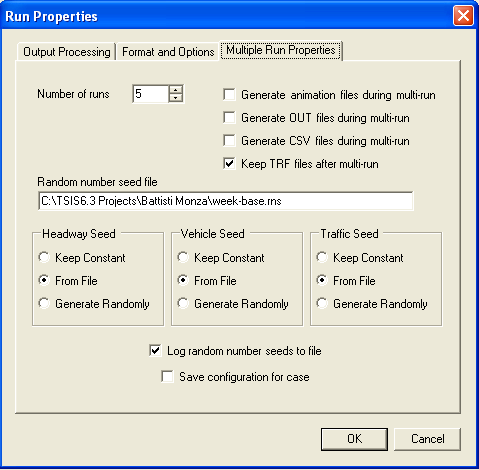
\includegraphics[width=1\columnwidth]{multi-run-properties-tsis-next}
	\caption[Esecuzione multipla guidata da file \acs{RNS}]{Selezione del file \acs{RNS} per l'impostazione dell'esecuzione multipla del \ds{2}.}\label{fig:multi-run-properties-tsis-next}
\end{figure}

Si osservi che per ogni esecuzione della simulazione viene generato il relativo file di output. Il nome di tali file \acs{CSV} è una concatenazione delle seguenti informazioni: nome del file \acs{TRF} (seguito dal numero dell'esecuzione in caso di esecuzione multipla), data e ora dell'esecuzione, suffisso \lstinline[]|sensors|.

\subsection{Applicativi di supporto}
Ottenuti i file di output di \acsfont{Sensors} \acs{DLL} è necessario trasformarli in un dataset utile al framework delle \acs{CTBN}. A tale scopo sono stati sviluppati degli applicativi, brevemente discussi nella \vref{sec:dataset-tools}.

Il primo passo necessario consiste nella sostituzione dei \emph{\keyword{time period}} con le rispettive classi (si veda a tal riguardo la \vref{tab:ds-2-tp-labels}). A tale scopo è stato sviluppato un programma in linguaggio \lstinline[]|R| con interfaccia \lstinline[]|bash| chiamato \lstinline[]|sensors2dataset|.

Riguardo al modello in questione è quindi necessario eseguire il succitato programma nel seguente modo, ripetendo tale passo per tutti i $5$ file di output generati (si ricorda che il modello per i giorni lavorativi viene eseguito infatti $5$ volte, una per ogni giorno lavorativo):

\cleardoublepage
\inputsourcecode[caption={[Sostituzione delle classi ai time period]Esecuzione del programma \lstinline[]|bash| per la sostituzione dei \emph{\keyword{time period}} con le relative classi nel file \acs{CSV} relativo al \ds{2}.},language=sh,basicstyle=\footnotesize\ttfamily,numbers=none,label=lst:sensors2dataset]{codes/sensors2dataset2}
Di seguito si spiegano brevemente le opzioni utilizzate:
\begin{itemize}
	\item l'opzione \lstinline[]|i| serve a specificare il percorso del file di input, cioè del file \acs{CSV} generato da \acsfont{Sensors} \acs{DLL}
	\item l'opzione \lstinline[]|t| comunica al programma che il file di input è dotato di intestazione
	\item l'opzione \lstinline[]|r| comunica al programma di rimuovere la colonna relativa ai \emph{\keyword{time period}}
	\item l'opzione \lstinline[]|b| serve a definire i \emph{\keyword{time period}} a partire dai quali una nuova classe deve essere creata e associata
	\item l'opzione \lstinline[]|v| serve per eseguire il programma in modo verboso.
\end{itemize}
Si osservi tuttavia che \lstinline[]|sensors2dataset| implementa molte altre opzioni la cui descrizione è stata tuttavia tralasciata.

Infine, si noti che \lstinline[]|sensors2dataset| non sovrascrive il file di input. Infatti, esso genera automaticamente un nuovo file con le modifiche apportate, concatenando al nome del file di input il suffisso \lstinline[]|dataset|.

A questo punto è possibile scegliere una granularità temporale qualsiasi con cui tagliare il file \acs{CSV}, tenendo presente che \acsfont{Sensors} \acs{DLL} utilizza per il monitoraggio del passaggio dei veicoli sui sensori la massima granularità temporale ottenibile da \acs{CORSIM}, cioè $0.1$ secondi.

Di conseguenza, ipotizzando di voler tagliare il corrente file \acs{CSV} in più file da $100$ secondi, si utilizza il programma \lstinline[]|bash| appositamente sviluppato a tale fine, \lstinline[]|splitfile|.
\vspace*{8pt}\inputsourcecode[caption={[Generazione del \ds{2}]Esecuzione del programma \lstinline[]|bash| finalizzato alla generazione del \ds{2}. Il file di input viene tagliato in più file, ognuno dei quali rappresentante un intervallo temporale di $100$ secondi.},language=sh,numbers=none,basicstyle=\small\ttfamily]{codes/splitfile2}
L'opzione \lstinline[]|n| serve a specificare il numero di righe da cui ogni file deve essere composto. In questo caso quindi, poiché ogni riga rappresenta un intervallo temporale di $0.1$ secondi e desideriamo ottenere dei file che rappresentino intervalli temporali minori o uguali di $100$ secondi, impostiamo il suo valore pari a $1000$.

Si osservi che \lstinline[]|splitfile| salva i file generati in una nuova cartella la cui posizione corrisponde a quella del file di input.

Infine, è possibile ottimizzare il dataset appena generato rimuovendo le righe che corrispondono a intervalli temporali durante i quali non è avvenuta alcuna transizione di stato per nessun sensore. A tale scopo viene fornito un programma \lstinline[]|bash| chiamato \lstinline[]|killconsdup|. Esso permette l'ottimizzazione di un singole file \acs{CSV} secondo la logica descritta oppure l'ottimizzazione di tutti i file \acs{CSV} presenti nella cartella di input fornita. Di seguito si illustra la seconda tipologia d'utilizzo di \lstinline[]|killconsdup|.
\vspace*{8pt}\inputsourcecode[caption={[Ottimizzazione del \ds{2}]Esecuzione del programma \lstinline[]|bash| finalizzato alla rimozione delle osservazioni duplicate, cioè delle righe relative agli intervalli temporali durante i quali tutti i sensori sono rimasti nel loro precedente stato.},language=sh,numbers=none]{codes/killconsdup2}
Si osservi che \lstinline$killconsdup$ non considera la prima riga dei file che processa, assumendo che essa contenga l'intestazione del file \acs{CSV}. Inoltre esso non considera la prima e la seconda colonna dei file di input assumendo esse si riferiscano rispettivamente alla colonna del tempo e della classe. Infine, affinché tale programma funzioni correttamente è necessario che il separatore dei file \acs{CSV} di input sia la virgola.

Eseguito il precedente comando, i file che compongono il dataset saranno sovrascritti con la loro rispettiva versione ottimizzata.

%% !TEX encoding = UTF-8
% !TEX TS-program = pdflatex
% !TEX root = ../arsclassica.tex
% !TEX spellcheck = it-IT

%************************************************
\chapter{Materiale}
\label{cap:stuff}
%************************************************

Lo scopo di questa appendice è illustrare il materiale (\eg{} sorgenti) relativo a questo lavoro di tesi.

\section{Modelli di traffico}\label{sec:trf-files}

In questa sezione si riportano i file che descrivono completamente le reti stradali e i relativi modelli di simulazione da cui si ottengono i \ds{1} e \mynum{2}. Lo scopo di questa sezione è permettere la completa riproducibilità dei dataset descritti nel \autoref{cap:esperimenti}.

\subsection{\Ds{1}}\label{sec:trf-1}

Si riporta il file \acs{TRF} da cui è possibile generare il \ds{1} (descritto nella \vref{sec:dataset-1}) utilizzando \acs{CORSIM} e \acsfont{Sensors} \acs{DLL}.

\lstinputsourcecode[language=pseudo, numbers=none, basicstyle=\scriptsize\ttfamily, caption={[Sorgente \acs{TRF} del \ds{1}]Sorgente \acs{TRF} che codifica la rete stradale da cui viene generato il \ds{1}.}]{codes/simple.trf}

\subsection{\Ds{2}}\label{sec:trf-2}

Si riportano i file \acs{TRF} da cui è possibile generare il \ds{2} (descritto nella \vref{sec:dataset-2}) utilizzando \acs{CORSIM} e \acsfont{Sensors} \acs{DLL}. Ognuno dei file riportati di seguito rappresentano la stessa rete stradale con diversi modelli di traffico.

In prims si riporta il file \acs{TRF} che codifica il modello di traffico dei giorni lavorativi.

\lstinputsourcecode[language=pseudo, numbers=none, basicstyle=\scriptsize\ttfamily, caption={[Sorgente \acs{TRF} del \ds{2} (giorni lavorativi)]Sorgente del file \acs{TRF} che codifica la rete stradale, e il modello di traffico durante i giorni lavorativi, da cui viene generato il \ds{2}.}]{codes/monza-week-exte.trf}

Di seguito si riporta il file \acs{TRF} che codifica il modello di traffico per il sabato.

\lstinputsourcecode[language=pseudo, numbers=none, basicstyle=\scriptsize\ttfamily, caption={[Sorgente \acs{TRF} del \ds{2} (sabato)]Sorgente del file \acs{TRF} che codifica la rete stradale, e il modello di traffico vigente il sabato, da cui viene generato il \ds{2}.}]{codes/monza-satu-exte.trf}

Segue il file \acs{TRF} che codifica il modello di traffico della domenica.

\lstinputsourcecode[language=pseudo, numbers=none, basicstyle=\scriptsize\ttfamily, caption={[Sorgente \acs{TRF} del \ds{2} (domenica)]Sorgente del file \acs{TRF} che codifica la rete stradale, e il modello di traffico vigente la domenica, da cui viene generato il \ds{2}.}]{codes/monza-sund-exte.trf}

Affinchè il dataset in questione sia perfettamente riproducibile si riportano anche i file \acs{RNS}\footnote{\acs{CORSIM} può leggere i semi numerici (\ie{} \emph{seed}) su cui basare la simulazione e il numero di esecuzioni da effettuare da dei file chiamati \acf{RNS}. Un file \acs{RNS} è un semplice file di testo opportunamente formattato: sulla prima riga va inserito il numero di esecuzioni da effettuare, le $3$ righe successive devono invece contenere $3$ numeri di \emph{seed} separati da un carattere di tabulazione.}

% !TEX encoding = UTF-8
% !TEX TS-program = pdflatex
% !TEX root = ../arsclassica.tex
% !TEX spellcheck = it-IT

%*******************************************************
% Acronyms
%*******************************************************
\cleardoublepage
\manualmark
\phantomsection
\addcontentsline{toc}{chapter}{\tocEntry{\acroname}}
\chapter*{\acroname\markboth{\spacedlowsmallcaps{\acroname}}{\spacedlowsmallcaps{\acroname}}}
\small
\begin{acronym}[CTTANBC] % insert in the square brackets the longest acronym word
    \acro{API}[API]{Application Programming Interface}
    \acro{BN}[BN]{\bn{}}
    \acro{BNC}[BNC]{\bn{} \class{}}
    \acro{CIM}[CIM]{\ul{Conditional Intensity Matrix}{matrice di intensit\`a condizionale}}
    \acro{CORSIM}[CORSIM]{Corridor microscopic simulation program}
    \acro{CPD}[CPD]{\ul{Conditional Probability Distribution}{distribuzione di probabilità condizionale}}
    \acro{CPT}[CPT]{\ul{Conditional Probability Table}{tabelle di probabilità condizionale}}
    \acro{CTBN}[CTBN]{\ctbn{}}
    \acro{CTBNC}[CTBNC]{\ctbn{} \class{}}
    \acro{CTNB}[CTNB]{\ctnb{}}
    \acro{CTNBC}[CTNBC]{\ctnb{} \class{}}
    \acro{CTTANB}[CTTANB]{\cttanb{}}
    \acro{CTTANBC}[CTTANBC]{\cttanb{} \class{}}
    \acro{DAG}[DAG]{\ul{Directed acyclic graph}{grafo aciclico orientato}}
    \acro{DBN}[DBN]{Dynamic Bayesian Networks}
    \acro{DLL}[DLL]{\ul{Dynamic-link library}{libreria a collegamento dinamico}}
    \acro{EM}[EM]{Expectation Maximization}
    \acro{FREESIM}[FREESIM]{Freeway Simulator}
    \acro{FWHA}[FWHA]{Federal Highway Administration}
    \acro{GUI}[GUI]{Graphical User Interface}
    \acro{IDE}[IDE]{\ul{Integrated Development Environment}{ambiente di sviluppo integrato}}
    \acro{IC}[IC]{Inductive Causation}
    \acro{IM}[IM]{\ul{Intensity Matrix}{matrice di intensit\`a}}
    \acro{MAP}[MAP]{\ul{Maximum a posteriori}{maximum a posteriori}}
    \acro{MCMC}[MCMC]{Markov Chain Monte Carlo}
    \acro{MLE}[MLE]{\ul{Maximum Likelihood Estimation}{maximum-likelihood}}
    \acro{NB}[NB]{Na\"ive Bayes}
    \acro{NETSIM}[NETSIM]{Network Simulator}
    \acro{PV}[PV]{\ul{Process Variable}{Variabile di processo}}
    \acro{RT}[RT]{Record Type}
    \acro{RTE}[RTE]{\ul{Run-Time Extension}{estensione a tempo d'esecuzione}}
    \acro{TAN}[TAN]{Tree Augumented \nb{}}
    \acro{TNO}[TNO]{TRAFED Native Object}
    \acro{TRAF}[TRAF]{Traffic File}
    \acro{TRAFED}[TRAFED]{TRAF Editor}
    \acro{TRAFVU}[TRAFVU]{TRAF Visualization Utility}
    \acro{TRF}[TRF]{Traffic File}
    \acro{TShell}[TShell]{TSIS Shell}
    \acro{TSIS}[TSIS]{Traffic Software Integrated System}
\end{acronym}

% !TEX encoding = UTF-8
% !TEX TS-program = pdflatex
% !TEX root = ../tesi.tex
% !TEX spellcheck = it-IT

%*******************************************************
% Indice analitico
%*******************************************************
\cleardoublepage
\manualmark
\phantomsection
\markboth{\spacedlowsmallcaps{\indexname}}{\spacedlowsmallcaps{\indexname}}
\addcontentsline{toc}{chapter}{\tocEntry{\indexname}}
\pagestyle{scrheadings}
\printindex

% !TEX encoding = UTF-8
% !TEX TS-program = pdflatex
% !TEX root = ../arsclassica.tex
% !TEX spellcheck = it-IT

%*******************************************************
% Bibliography
%*******************************************************
\cleardoublepage
%\nocite{*}
\printbibliography

% !TEX encoding = UTF-8
% !TEX TS-program = pdflatex
% !TEX root = ../arsclassica.tex
% !TEX spellcheck = it-IT

%*******************************************************
% Declaration
%*******************************************************
\cleardoublepage
\phantomsection
\pdfbookmark{Dichiarazione}{Dichiarazione}
\chapter*{Dichiarazione}
\thispagestyle{empty}

Lorem ipsum dolor sit amet, consectetuer adipiscing elit. Ut purus elit, vestibulum ut, placerat ac, adipiscing vitae, felis. Curabitur dictum gravida mauris. Nam arcu libero, nonummy eget, consectetuer id, vulputate a, magna. Donec vehicula augue eu neque.

Pellentesque habitant morbi tristique senectus et netus et malesuada fames ac turpis egestas. Mauris ut leo. Cras viverra metus rhoncus sem. Nulla et lectus vestibulum urna fringilla ultrices.

\bigskip
 
\noindent\textit{\mylocation, \MakeTextLowercase{\mytime}}

\smallskip

\begin{flushright}
    \begin{tabular}{m{5cm}}
        \\ \hline
        \centering\myname \\
    \end{tabular}
\end{flushright}

\end{document}
